\documentclass[twoside]{book}

% Packages required by doxygen
\usepackage{fixltx2e}
\usepackage{calc}
\usepackage{doxygen}
\usepackage[export]{adjustbox} % also loads graphicx
\usepackage{graphicx}
\usepackage[utf8]{inputenc}
\usepackage{makeidx}
\usepackage{multicol}
\usepackage{multirow}
\PassOptionsToPackage{warn}{textcomp}
\usepackage{textcomp}
\usepackage[nointegrals]{wasysym}
\usepackage[table]{xcolor}

% Font selection
\usepackage[T1]{fontenc}
\usepackage[scaled=.90]{helvet}
\usepackage{courier}
\usepackage{amssymb}
\usepackage{sectsty}
\renewcommand{\familydefault}{\sfdefault}
\allsectionsfont{%
  \fontseries{bc}\selectfont%
  \color{darkgray}%
}
\renewcommand{\DoxyLabelFont}{%
  \fontseries{bc}\selectfont%
  \color{darkgray}%
}
\newcommand{\+}{\discretionary{\mbox{\scriptsize$\hookleftarrow$}}{}{}}

% Page & text layout
\usepackage{geometry}
\geometry{%
  a4paper,%
  top=2.5cm,%
  bottom=2.5cm,%
  left=2.5cm,%
  right=2.5cm%
}
\tolerance=750
\hfuzz=15pt
\hbadness=750
\setlength{\emergencystretch}{15pt}
\setlength{\parindent}{0cm}
\setlength{\parskip}{3ex plus 2ex minus 2ex}
\makeatletter
\renewcommand{\paragraph}{%
  \@startsection{paragraph}{4}{0ex}{-1.0ex}{1.0ex}{%
    \normalfont\normalsize\bfseries\SS@parafont%
  }%
}
\renewcommand{\subparagraph}{%
  \@startsection{subparagraph}{5}{0ex}{-1.0ex}{1.0ex}{%
    \normalfont\normalsize\bfseries\SS@subparafont%
  }%
}
\makeatother

% Headers & footers
\usepackage{fancyhdr}
\pagestyle{fancyplain}
\fancyhead[LE]{\fancyplain{}{\bfseries\thepage}}
\fancyhead[CE]{\fancyplain{}{}}
\fancyhead[RE]{\fancyplain{}{\bfseries\leftmark}}
\fancyhead[LO]{\fancyplain{}{\bfseries\rightmark}}
\fancyhead[CO]{\fancyplain{}{}}
\fancyhead[RO]{\fancyplain{}{\bfseries\thepage}}
\fancyfoot[LE]{\fancyplain{}{}}
\fancyfoot[CE]{\fancyplain{}{}}
\fancyfoot[RE]{\fancyplain{}{\bfseries\scriptsize Generated by Doxygen }}
\fancyfoot[LO]{\fancyplain{}{\bfseries\scriptsize Generated by Doxygen }}
\fancyfoot[CO]{\fancyplain{}{}}
\fancyfoot[RO]{\fancyplain{}{}}
\renewcommand{\footrulewidth}{0.4pt}
\renewcommand{\chaptermark}[1]{%
  \markboth{#1}{}%
}
\renewcommand{\sectionmark}[1]{%
  \markright{\thesection\ #1}%
}

% Indices & bibliography
\usepackage{natbib}
\usepackage[titles]{tocloft}
\setcounter{tocdepth}{3}
\setcounter{secnumdepth}{5}
\makeindex

% Hyperlinks (required, but should be loaded last)
\usepackage{ifpdf}
\ifpdf
  \usepackage[pdftex,pagebackref=true]{hyperref}
\else
  \usepackage[ps2pdf,pagebackref=true]{hyperref}
\fi
\hypersetup{%
  colorlinks=true,%
  linkcolor=blue,%
  citecolor=blue,%
  unicode%
}

% Custom commands
\newcommand{\clearemptydoublepage}{%
  \newpage{\pagestyle{empty}\cleardoublepage}%
}

\usepackage{caption}
\captionsetup{labelsep=space,justification=centering,font={bf},singlelinecheck=off,skip=4pt,position=top}

%===== C O N T E N T S =====

\begin{document}

% Titlepage & ToC
\hypersetup{pageanchor=false,
             bookmarksnumbered=true,
             pdfencoding=unicode
            }
\pagenumbering{alph}
\begin{titlepage}
\vspace*{7cm}
\begin{center}%
{\Large Bergermeister\+Home }\\
\vspace*{1cm}
{\large Generated by Doxygen 1.8.14}\\
\end{center}
\end{titlepage}
\clearemptydoublepage
\pagenumbering{roman}
\tableofcontents
\clearemptydoublepage
\pagenumbering{arabic}
\hypersetup{pageanchor=true}

%--- Begin generated contents ---
\chapter{Namespace Index}
\section{Namespace List}
Here is a list of all documented namespaces with brief descriptions\+:\begin{DoxyCompactList}
\item\contentsline{section}{\mbox{\hyperlink{namespace_g_n_common}{G\+N\+Common}} }{\pageref{namespace_g_n_common}}{}
\end{DoxyCompactList}

\chapter{Hierarchical Index}
\section{Class Hierarchy}
This inheritance list is sorted roughly, but not completely, alphabetically\+:\begin{DoxyCompactList}
\item \contentsline{section}{G\+N\+Common\+:\+:N\+Component\+:\+:G\+Tc\+Event$<$ aui\+Max\+Listeners $>$}{\pageref{class_g_n_common_1_1_n_component_1_1_g_tc_event}}{}
\item \contentsline{section}{G\+N\+Common\+:\+:N\+Component\+:\+:G\+Tc\+Event$<$ xui\+Max\+Listeners $>$}{\pageref{class_g_n_common_1_1_n_component_1_1_g_tc_event}}{}
\item \contentsline{section}{G\+N\+Common\+:\+:N\+Containers\+:\+:G\+Tc\+Linked\+List$<$ G\+Tc\+Type $>$}{\pageref{class_g_n_common_1_1_n_containers_1_1_g_tc_linked_list}}{}
\item \contentsline{section}{G\+N\+Common\+:\+:N\+Containers\+:\+:G\+Tc\+Linked\+List$<$ G\+N\+Common\+:\+:N\+Component\+:\+:G\+Tc\+Listener $>$}{\pageref{class_g_n_common_1_1_n_containers_1_1_g_tc_linked_list}}{}
\item \contentsline{section}{G\+N\+Common\+:\+:N\+Containers\+:\+:G\+Tc\+List$<$ G\+Tc\+Type $>$}{\pageref{class_g_n_common_1_1_n_containers_1_1_g_tc_list}}{}
\item \contentsline{section}{G\+N\+Common\+:\+:N\+Component\+:\+:G\+Tc\+Listener}{\pageref{class_g_n_common_1_1_n_component_1_1_g_tc_listener}}{}
\item \contentsline{section}{G\+N\+Common\+:\+:N\+Containers\+:\+:G\+Tc\+List\+Node$<$ G\+Tc\+Type $>$}{\pageref{class_g_n_common_1_1_n_containers_1_1_g_tc_list_node}}{}
\item \contentsline{section}{G\+N\+Common\+:\+:N\+Containers\+:\+:G\+Tc\+List\+Node$<$ G\+N\+Common\+:\+:N\+Component\+:\+:G\+Tc\+Listener $>$}{\pageref{class_g_n_common_1_1_n_containers_1_1_g_tc_list_node}}{}
\item \contentsline{section}{G\+N\+Common\+:\+:N\+Containers\+:\+:G\+Tc\+Queue$<$ G\+Tc\+Type $>$}{\pageref{class_g_n_common_1_1_n_containers_1_1_g_tc_queue}}{}
\item \contentsline{section}{G\+N\+Common\+:\+:G\+Tc\+Stop\+Watch}{\pageref{class_g_n_common_1_1_g_tc_stop_watch}}{}
\item \contentsline{section}{G\+N\+Common\+:\+:N\+Data\+Authentication\+:\+:Tc\+C\+R\+C32}{\pageref{class_g_n_common_1_1_n_data_authentication_1_1_tc_c_r_c32}}{}
\item \contentsline{section}{G\+N\+Common\+:\+:N\+Notification\+:\+:Tc\+Identifier}{\pageref{class_g_n_common_1_1_n_notification_1_1_tc_identifier}}{}
\item \contentsline{section}{G\+N\+Common\+:\+:N\+Component\+:\+:Tc\+Model}{\pageref{class_g_n_common_1_1_n_component_1_1_tc_model}}{}
\begin{DoxyCompactList}
\item \contentsline{section}{G\+N\+Common\+:\+:N\+Notification\+:\+:Tc\+Alert}{\pageref{class_g_n_common_1_1_n_notification_1_1_tc_alert}}{}
\end{DoxyCompactList}
\item \contentsline{section}{G\+N\+Common\+:\+:N\+Notification\+:\+:Tc\+Status}{\pageref{class_g_n_common_1_1_n_notification_1_1_tc_status}}{}
\end{DoxyCompactList}

\chapter{Class Index}
\section{Class List}
Here are the classes, structs, unions and interfaces with brief descriptions\+:\begin{DoxyCompactList}
\item\contentsline{section}{\mbox{\hyperlink{class_console_1_1_app}{Console\+::\+App}} \\*Provides application-\/specific behavior to supplement the default Application class. }{\pageref{class_console_1_1_app}}{}
\item\contentsline{section}{\mbox{\hyperlink{class_thermostat_1_1_app}{Thermostat\+::\+App}} \\*Provides application-\/specific behavior to supplement the default Application class. }{\pageref{class_thermostat_1_1_app}}{}
\item\contentsline{section}{\mbox{\hyperlink{class_g_n_common_1_1_g_tc_alert}{G\+N\+Common\+::\+G\+Tc\+Alert}} }{\pageref{class_g_n_common_1_1_g_tc_alert}}{}
\item\contentsline{section}{\mbox{\hyperlink{class_g_n_common_1_1_g_n_drivers_1_1_g_tc_d_h_t_sensor}{G\+N\+Common\+::\+G\+N\+Drivers\+::\+G\+Tc\+D\+H\+T\+Sensor}} }{\pageref{class_g_n_common_1_1_g_n_drivers_1_1_g_tc_d_h_t_sensor}}{}
\item\contentsline{section}{\mbox{\hyperlink{class_console_1_1_g_tc_d_h_t_sensor}{Console\+::\+G\+Tc\+D\+H\+T\+Sensor}} }{\pageref{class_console_1_1_g_tc_d_h_t_sensor}}{}
\item\contentsline{section}{\mbox{\hyperlink{class_g_n_common_1_1_g_n_component_1_1_g_tc_event}{G\+N\+Common\+::\+G\+N\+Component\+::\+G\+Tc\+Event$<$ aui\+Max\+Listeners $>$}} }{\pageref{class_g_n_common_1_1_g_n_component_1_1_g_tc_event}}{}
\item\contentsline{section}{\mbox{\hyperlink{class_g_n_common_1_1_g_n_containers_1_1_g_tc_linked_list}{G\+N\+Common\+::\+G\+N\+Containers\+::\+G\+Tc\+Linked\+List$<$ G\+Tc\+Type $>$}} }{\pageref{class_g_n_common_1_1_g_n_containers_1_1_g_tc_linked_list}}{}
\item\contentsline{section}{\mbox{\hyperlink{class_g_n_common_1_1_g_n_containers_1_1_g_tc_list}{G\+N\+Common\+::\+G\+N\+Containers\+::\+G\+Tc\+List$<$ G\+Tc\+Type $>$}} }{\pageref{class_g_n_common_1_1_g_n_containers_1_1_g_tc_list}}{}
\item\contentsline{section}{\mbox{\hyperlink{class_g_n_common_1_1_g_n_component_1_1_g_tc_listener}{G\+N\+Common\+::\+G\+N\+Component\+::\+G\+Tc\+Listener}} }{\pageref{class_g_n_common_1_1_g_n_component_1_1_g_tc_listener}}{}
\item\contentsline{section}{\mbox{\hyperlink{class_g_n_common_1_1_g_n_containers_1_1_g_tc_list_node}{G\+N\+Common\+::\+G\+N\+Containers\+::\+G\+Tc\+List\+Node$<$ G\+Tc\+Type $>$}} }{\pageref{class_g_n_common_1_1_g_n_containers_1_1_g_tc_list_node}}{}
\item\contentsline{section}{\mbox{\hyperlink{class_g_n_common_1_1_g_n_component_1_1_g_tc_model}{G\+N\+Common\+::\+G\+N\+Component\+::\+G\+Tc\+Model}} }{\pageref{class_g_n_common_1_1_g_n_component_1_1_g_tc_model}}{}
\item\contentsline{section}{\mbox{\hyperlink{class_g_n_common_1_1_g_n_serial_1_1_g_tc_port}{G\+N\+Common\+::\+G\+N\+Serial\+::\+G\+Tc\+Port}} }{\pageref{class_g_n_common_1_1_g_n_serial_1_1_g_tc_port}}{}
\item\contentsline{section}{\mbox{\hyperlink{class_g_n_common_1_1_g_n_containers_1_1_g_tc_queue}{G\+N\+Common\+::\+G\+N\+Containers\+::\+G\+Tc\+Queue$<$ G\+Tc\+Type $>$}} }{\pageref{class_g_n_common_1_1_g_n_containers_1_1_g_tc_queue}}{}
\item\contentsline{section}{\mbox{\hyperlink{class_g_n_common_1_1_g_tc_stop_watch}{G\+N\+Common\+::\+G\+Tc\+Stop\+Watch}} }{\pageref{class_g_n_common_1_1_g_tc_stop_watch}}{}
\item\contentsline{section}{\mbox{\hyperlink{struct_identifier}{Identifier}} }{\pageref{struct_identifier}}{}
\item\contentsline{section}{\mbox{\hyperlink{class_xaml_binding_info_1_1_i_xaml_bindings}{Xaml\+Binding\+Info\+::\+I\+Xaml\+Bindings}} }{\pageref{class_xaml_binding_info_1_1_i_xaml_bindings}}{}
\item\contentsline{section}{\mbox{\hyperlink{class_console_1_1_main_page}{Console\+::\+Main\+Page}} \\*An empty page that can be used on its own or navigated to within a Frame. }{\pageref{class_console_1_1_main_page}}{}
\item\contentsline{section}{\mbox{\hyperlink{class_thermostat_1_1_main_page}{Thermostat\+::\+Main\+Page}} \\*An empty page that can be used on its own or navigated to within a Frame. }{\pageref{class_thermostat_1_1_main_page}}{}
\item\contentsline{section}{\mbox{\hyperlink{struct_status}{Status}} }{\pageref{struct_status}}{}
\item\contentsline{section}{\mbox{\hyperlink{struct_g_n_common_1_1_g_tc_alert_1_1_ts_identifier}{G\+N\+Common\+::\+G\+Tc\+Alert\+::\+Ts\+Identifier}} }{\pageref{struct_g_n_common_1_1_g_tc_alert_1_1_ts_identifier}}{}
\item\contentsline{section}{\mbox{\hyperlink{struct_g_n_common_1_1_g_tc_alert_1_1_ts_status}{G\+N\+Common\+::\+G\+Tc\+Alert\+::\+Ts\+Status}} }{\pageref{struct_g_n_common_1_1_g_tc_alert_1_1_ts_status}}{}
\item\contentsline{section}{\mbox{\hyperlink{struct_type_info}{Type\+Info}} }{\pageref{struct_type_info}}{}
\item\contentsline{section}{\mbox{\hyperlink{class_xaml_binding_info_1_1_xaml_bindings}{Xaml\+Binding\+Info\+::\+Xaml\+Bindings}} }{\pageref{class_xaml_binding_info_1_1_xaml_bindings}}{}
\item\contentsline{section}{\mbox{\hyperlink{class_xaml_type_info_1_1_info_provider_1_1_xaml_member}{Xaml\+Type\+Info\+::\+Info\+Provider\+::\+Xaml\+Member}} }{\pageref{class_xaml_type_info_1_1_info_provider_1_1_xaml_member}}{}
\item\contentsline{section}{\mbox{\hyperlink{class_xaml_type_info_1_1_info_provider_1_1_xaml_system_base_type}{Xaml\+Type\+Info\+::\+Info\+Provider\+::\+Xaml\+System\+Base\+Type}} }{\pageref{class_xaml_type_info_1_1_info_provider_1_1_xaml_system_base_type}}{}
\item\contentsline{section}{\mbox{\hyperlink{class_xaml_type_info_1_1_info_provider_1_1_xaml_type_info_provider}{Xaml\+Type\+Info\+::\+Info\+Provider\+::\+Xaml\+Type\+Info\+Provider}} }{\pageref{class_xaml_type_info_1_1_info_provider_1_1_xaml_type_info_provider}}{}
\item\contentsline{section}{\mbox{\hyperlink{class_xaml_type_info_1_1_info_provider_1_1_xaml_user_type}{Xaml\+Type\+Info\+::\+Info\+Provider\+::\+Xaml\+User\+Type}} }{\pageref{class_xaml_type_info_1_1_info_provider_1_1_xaml_user_type}}{}
\end{DoxyCompactList}

\chapter{File Index}
\section{File List}
Here is a list of all documented files with brief descriptions\+:\begin{DoxyCompactList}
\item\contentsline{section}{C\+:/\+Projects/\+Bergermeister\+Home/\+Common/\+Source/{\bfseries Alert.\+cpp} }{\pageref{_alert_8cpp}}{}
\item\contentsline{section}{C\+:/\+Projects/\+Bergermeister\+Home/\+Common/\+Source/\mbox{\hyperlink{_alert_8h}{Alert.\+h}} }{\pageref{_alert_8h}}{}
\item\contentsline{section}{C\+:/\+Projects/\+Bergermeister\+Home/\+Common/\+Source/{\bfseries Constants.\+h} }{\pageref{_constants_8h}}{}
\item\contentsline{section}{C\+:/\+Projects/\+Bergermeister\+Home/\+Common/\+Source/{\bfseries pch.\+cpp} }{\pageref{_common_2_source_2pch_8cpp}}{}
\item\contentsline{section}{C\+:/\+Projects/\+Bergermeister\+Home/\+Common/\+Source/{\bfseries pch.\+h} }{\pageref{_common_2_source_2pch_8h}}{}
\item\contentsline{section}{C\+:/\+Projects/\+Bergermeister\+Home/\+Common/\+Source/{\bfseries Stop\+Watch.\+cpp} }{\pageref{_stop_watch_8cpp}}{}
\item\contentsline{section}{C\+:/\+Projects/\+Bergermeister\+Home/\+Common/\+Source/{\bfseries Stop\+Watch.\+h} }{\pageref{_stop_watch_8h}}{}
\item\contentsline{section}{C\+:/\+Projects/\+Bergermeister\+Home/\+Common/\+Source/\mbox{\hyperlink{_types_8h}{Types.\+h}} }{\pageref{_types_8h}}{}
\item\contentsline{section}{C\+:/\+Projects/\+Bergermeister\+Home/\+Common/\+Source/\+Component/{\bfseries Event.\+h} }{\pageref{_event_8h}}{}
\item\contentsline{section}{C\+:/\+Projects/\+Bergermeister\+Home/\+Common/\+Source/\+Component/{\bfseries Listener.\+cpp} }{\pageref{_listener_8cpp}}{}
\item\contentsline{section}{C\+:/\+Projects/\+Bergermeister\+Home/\+Common/\+Source/\+Component/{\bfseries Listener.\+h} }{\pageref{_listener_8h}}{}
\item\contentsline{section}{C\+:/\+Projects/\+Bergermeister\+Home/\+Common/\+Source/\+Component/{\bfseries Model.\+cpp} }{\pageref{_model_8cpp}}{}
\item\contentsline{section}{C\+:/\+Projects/\+Bergermeister\+Home/\+Common/\+Source/\+Component/{\bfseries Model.\+h} }{\pageref{_model_8h}}{}
\item\contentsline{section}{C\+:/\+Projects/\+Bergermeister\+Home/\+Common/\+Source/\+Containers/{\bfseries Linked\+List.\+h} }{\pageref{_linked_list_8h}}{}
\item\contentsline{section}{C\+:/\+Projects/\+Bergermeister\+Home/\+Common/\+Source/\+Containers/{\bfseries List.\+h} }{\pageref{_list_8h}}{}
\item\contentsline{section}{C\+:/\+Projects/\+Bergermeister\+Home/\+Common/\+Source/\+Containers/{\bfseries List\+Node.\+h} }{\pageref{_list_node_8h}}{}
\item\contentsline{section}{C\+:/\+Projects/\+Bergermeister\+Home/\+Common/\+Source/\+Containers/{\bfseries Queue.\+h} }{\pageref{_queue_8h}}{}
\item\contentsline{section}{C\+:/\+Projects/\+Bergermeister\+Home/\+Common/\+Source/\+Drivers-\/bak/{\bfseries D\+H\+T\+Sensor.\+cpp} }{\pageref{_common_2_source_2_drivers-bak_2_d_h_t_sensor_8cpp}}{}
\item\contentsline{section}{C\+:/\+Projects/\+Bergermeister\+Home/\+Common/\+Source/\+Drivers-\/bak/{\bfseries D\+H\+T\+Sensor.\+h} }{\pageref{_common_2_source_2_drivers-bak_2_d_h_t_sensor_8h}}{}
\item\contentsline{section}{C\+:/\+Projects/\+Bergermeister\+Home/\+Console/{\bfseries App.\+xaml.\+cpp} }{\pageref{_console_2_app_8xaml_8cpp}}{}
\item\contentsline{section}{C\+:/\+Projects/\+Bergermeister\+Home/\+Console/{\bfseries App.\+xaml.\+h} }{\pageref{_console_2_app_8xaml_8h}}{}
\item\contentsline{section}{C\+:/\+Projects/\+Bergermeister\+Home/\+Console/{\bfseries D\+H\+T\+Sensor.\+cpp} }{\pageref{_console_2_d_h_t_sensor_8cpp}}{}
\item\contentsline{section}{C\+:/\+Projects/\+Bergermeister\+Home/\+Console/{\bfseries D\+H\+T\+Sensor.\+h} }{\pageref{_console_2_d_h_t_sensor_8h}}{}
\item\contentsline{section}{C\+:/\+Projects/\+Bergermeister\+Home/\+Console/{\bfseries Main\+Page.\+xaml.\+cpp} }{\pageref{_console_2_main_page_8xaml_8cpp}}{}
\item\contentsline{section}{C\+:/\+Projects/\+Bergermeister\+Home/\+Console/{\bfseries Main\+Page.\+xaml.\+h} }{\pageref{_console_2_main_page_8xaml_8h}}{}
\item\contentsline{section}{C\+:/\+Projects/\+Bergermeister\+Home/\+Console/{\bfseries pch.\+cpp} }{\pageref{_console_2pch_8cpp}}{}
\item\contentsline{section}{C\+:/\+Projects/\+Bergermeister\+Home/\+Console/{\bfseries pch.\+h} }{\pageref{_console_2pch_8h}}{}
\item\contentsline{section}{C\+:/\+Projects/\+Bergermeister\+Home/\+Console/\+Generated Files/{\bfseries App.\+g.\+h} }{\pageref{_console_2_generated_01_files_2_app_8g_8h}}{}
\item\contentsline{section}{C\+:/\+Projects/\+Bergermeister\+Home/\+Console/\+Generated Files/{\bfseries Main\+Page.\+g.\+h} }{\pageref{_console_2_generated_01_files_2_main_page_8g_8h}}{}
\item\contentsline{section}{C\+:/\+Projects/\+Bergermeister\+Home/\+Console/\+Generated Files/{\bfseries Xaml\+Binding\+Info.\+g.\+h} }{\pageref{_console_2_generated_01_files_2_xaml_binding_info_8g_8h}}{}
\item\contentsline{section}{C\+:/\+Projects/\+Bergermeister\+Home/\+Console/\+Generated Files/{\bfseries Xaml\+Binding\+Info.\+g.\+hpp} }{\pageref{_console_2_generated_01_files_2_xaml_binding_info_8g_8hpp}}{}
\item\contentsline{section}{C\+:/\+Projects/\+Bergermeister\+Home/\+Console/\+Generated Files/{\bfseries Xaml\+Lib\+Metadata\+Provider.\+g.\+cpp} }{\pageref{_console_2_generated_01_files_2_xaml_lib_metadata_provider_8g_8cpp}}{}
\item\contentsline{section}{C\+:/\+Projects/\+Bergermeister\+Home/\+Console/\+Generated Files/{\bfseries Xaml\+Type\+Info.\+g.\+h} }{\pageref{_console_2_generated_01_files_2_xaml_type_info_8g_8h}}{}
\item\contentsline{section}{C\+:/\+Projects/\+Bergermeister\+Home/\+Console/\+Generated Files/{\bfseries Xaml\+Type\+Info.\+Impl.\+g.\+cpp} }{\pageref{_console_2_generated_01_files_2_xaml_type_info_8_impl_8g_8cpp}}{}
\item\contentsline{section}{C\+:/\+Projects/\+Bergermeister\+Home/\+Serial/{\bfseries dllmain.\+cpp} }{\pageref{dllmain_8cpp}}{}
\item\contentsline{section}{C\+:/\+Projects/\+Bergermeister\+Home/\+Serial/{\bfseries pch.\+cpp} }{\pageref{_serial_2pch_8cpp}}{}
\item\contentsline{section}{C\+:/\+Projects/\+Bergermeister\+Home/\+Serial/{\bfseries pch.\+h} }{\pageref{_serial_2pch_8h}}{}
\item\contentsline{section}{C\+:/\+Projects/\+Bergermeister\+Home/\+Serial/{\bfseries Port.\+cpp} }{\pageref{_port_8cpp}}{}
\item\contentsline{section}{C\+:/\+Projects/\+Bergermeister\+Home/\+Serial/{\bfseries Port.\+h} }{\pageref{_port_8h}}{}
\item\contentsline{section}{C\+:/\+Projects/\+Bergermeister\+Home/\+Serial/{\bfseries targetver.\+h} }{\pageref{targetver_8h}}{}
\item\contentsline{section}{C\+:/\+Projects/\+Bergermeister\+Home/\+Thermostat/{\bfseries App.\+xaml.\+cpp} }{\pageref{_thermostat_2_app_8xaml_8cpp}}{}
\item\contentsline{section}{C\+:/\+Projects/\+Bergermeister\+Home/\+Thermostat/{\bfseries App.\+xaml.\+h} }{\pageref{_thermostat_2_app_8xaml_8h}}{}
\item\contentsline{section}{C\+:/\+Projects/\+Bergermeister\+Home/\+Thermostat/{\bfseries Main\+Page.\+xaml.\+cpp} }{\pageref{_thermostat_2_main_page_8xaml_8cpp}}{}
\item\contentsline{section}{C\+:/\+Projects/\+Bergermeister\+Home/\+Thermostat/{\bfseries Main\+Page.\+xaml.\+h} }{\pageref{_thermostat_2_main_page_8xaml_8h}}{}
\item\contentsline{section}{C\+:/\+Projects/\+Bergermeister\+Home/\+Thermostat/{\bfseries pch.\+cpp} }{\pageref{_thermostat_2pch_8cpp}}{}
\item\contentsline{section}{C\+:/\+Projects/\+Bergermeister\+Home/\+Thermostat/{\bfseries pch.\+h} }{\pageref{_thermostat_2pch_8h}}{}
\item\contentsline{section}{C\+:/\+Projects/\+Bergermeister\+Home/\+Thermostat/\+Drivers/{\bfseries D\+H\+T\+Sensor.\+cpp} }{\pageref{_thermostat_2_drivers_2_d_h_t_sensor_8cpp}}{}
\item\contentsline{section}{C\+:/\+Projects/\+Bergermeister\+Home/\+Thermostat/\+Drivers/{\bfseries D\+H\+T\+Sensor.\+h} }{\pageref{_thermostat_2_drivers_2_d_h_t_sensor_8h}}{}
\item\contentsline{section}{C\+:/\+Projects/\+Bergermeister\+Home/\+Thermostat/\+Generated Files/{\bfseries App.\+g.\+h} }{\pageref{_thermostat_2_generated_01_files_2_app_8g_8h}}{}
\item\contentsline{section}{C\+:/\+Projects/\+Bergermeister\+Home/\+Thermostat/\+Generated Files/{\bfseries App.\+g.\+hpp} }{\pageref{_app_8g_8hpp}}{}
\item\contentsline{section}{C\+:/\+Projects/\+Bergermeister\+Home/\+Thermostat/\+Generated Files/{\bfseries Main\+Page.\+g.\+h} }{\pageref{_thermostat_2_generated_01_files_2_main_page_8g_8h}}{}
\item\contentsline{section}{C\+:/\+Projects/\+Bergermeister\+Home/\+Thermostat/\+Generated Files/{\bfseries Main\+Page.\+g.\+hpp} }{\pageref{_main_page_8g_8hpp}}{}
\item\contentsline{section}{C\+:/\+Projects/\+Bergermeister\+Home/\+Thermostat/\+Generated Files/{\bfseries Xaml\+Binding\+Info.\+g.\+h} }{\pageref{_thermostat_2_generated_01_files_2_xaml_binding_info_8g_8h}}{}
\item\contentsline{section}{C\+:/\+Projects/\+Bergermeister\+Home/\+Thermostat/\+Generated Files/{\bfseries Xaml\+Binding\+Info.\+g.\+hpp} }{\pageref{_thermostat_2_generated_01_files_2_xaml_binding_info_8g_8hpp}}{}
\item\contentsline{section}{C\+:/\+Projects/\+Bergermeister\+Home/\+Thermostat/\+Generated Files/{\bfseries Xaml\+Lib\+Metadata\+Provider.\+g.\+cpp} }{\pageref{_thermostat_2_generated_01_files_2_xaml_lib_metadata_provider_8g_8cpp}}{}
\item\contentsline{section}{C\+:/\+Projects/\+Bergermeister\+Home/\+Thermostat/\+Generated Files/{\bfseries Xaml\+Type\+Info.\+g.\+cpp} }{\pageref{_xaml_type_info_8g_8cpp}}{}
\item\contentsline{section}{C\+:/\+Projects/\+Bergermeister\+Home/\+Thermostat/\+Generated Files/{\bfseries Xaml\+Type\+Info.\+g.\+h} }{\pageref{_thermostat_2_generated_01_files_2_xaml_type_info_8g_8h}}{}
\item\contentsline{section}{C\+:/\+Projects/\+Bergermeister\+Home/\+Thermostat/\+Generated Files/{\bfseries Xaml\+Type\+Info.\+Impl.\+g.\+cpp} }{\pageref{_thermostat_2_generated_01_files_2_xaml_type_info_8_impl_8g_8cpp}}{}
\end{DoxyCompactList}

\chapter{Namespace Documentation}
\hypertarget{namespace_g_n_common}{}\section{G\+N\+Common Namespace Reference}
\label{namespace_g_n_common}\index{G\+N\+Common@{G\+N\+Common}}


Namespace containing Common components and infrastrucutre.  


\subsection*{Namespaces}
\begin{DoxyCompactItemize}
\item 
 \mbox{\hyperlink{namespace_g_n_common_1_1_n_data_authentication}{N\+Data\+Authentication}}
\begin{DoxyCompactList}\small\item\em Namespace containing Data Authentication and Validity utilities. \end{DoxyCompactList}\item 
 \mbox{\hyperlink{namespace_g_n_common_1_1_n_notification}{N\+Notification}}
\begin{DoxyCompactList}\small\item\em Namespace containing system Alerts. \end{DoxyCompactList}\end{DoxyCompactItemize}
\subsection*{Classes}
\begin{DoxyCompactItemize}
\item 
class \mbox{\hyperlink{class_g_n_common_1_1_g_tc_stop_watch}{G\+Tc\+Stop\+Watch}}
\end{DoxyCompactItemize}
\subsection*{Typedefs}
\begin{DoxyCompactItemize}
\item 
typedef bool \mbox{\hyperlink{namespace_g_n_common_a8115dc7ed53b6e5b52e6bfde1632ea74}{Tb8}}
\item 
typedef char \mbox{\hyperlink{namespace_g_n_common_a2d8d4c56e54519697c6ee80cc1ceda76}{Tc8}}
\item 
typedef signed char \mbox{\hyperlink{namespace_g_n_common_a9bac2aa36db6d72a3e59b1869adf3668}{Ti8}}
\item 
typedef unsigned char \mbox{\hyperlink{namespace_g_n_common_a7939e251ddbf5d3a31832dcfdc8bde39}{Tu8}}
\item 
typedef signed short \mbox{\hyperlink{namespace_g_n_common_ab9a9a6aa84751cec965d8b6676318a65}{Ti16}}
\item 
typedef unsigned short \mbox{\hyperlink{namespace_g_n_common_a7f651a58155939d1e0e2bf2164fbfdbf}{Tu16}}
\item 
typedef signed long \mbox{\hyperlink{namespace_g_n_common_ad1f094ce51908947ac3d31355b560d55}{Ti32}}
\item 
typedef unsigned long \mbox{\hyperlink{namespace_g_n_common_a941b527ef318f318aed7903dc832b7e4}{Tu32}}
\item 
typedef signed long long \mbox{\hyperlink{namespace_g_n_common_ad0a34f67eefe81cfbd0e515bba246d9d}{Ti64}}
\item 
typedef unsigned long long \mbox{\hyperlink{namespace_g_n_common_a9404ee6090c788ae70aebd1436ceb97d}{Tu64}}
\item 
typedef float \mbox{\hyperlink{namespace_g_n_common_ae4ffdde6236eb7578669b280a5d1634d}{Tf32}}
\item 
typedef double \mbox{\hyperlink{namespace_g_n_common_a73af96f1663fd8fc5741bcbc5b1427e4}{Tf64}}
\end{DoxyCompactItemize}


\subsection{Detailed Description}
Namespace containing Common components and infrastrucutre. 

\subsection{Typedef Documentation}
\mbox{\Hypertarget{namespace_g_n_common_a8115dc7ed53b6e5b52e6bfde1632ea74}\label{namespace_g_n_common_a8115dc7ed53b6e5b52e6bfde1632ea74}} 
\index{G\+N\+Common@{G\+N\+Common}!Tb8@{Tb8}}
\index{Tb8@{Tb8}!G\+N\+Common@{G\+N\+Common}}
\subsubsection{\texorpdfstring{Tb8}{Tb8}}
{\footnotesize\ttfamily typedef bool \mbox{\hyperlink{namespace_g_n_common_a8115dc7ed53b6e5b52e6bfde1632ea74}{G\+N\+Common\+::\+Tb8}}}

Type definition for 8-\/bit boolean primitive 

Definition at line \mbox{\hyperlink{_types_8h_source_l00054}{54}} of file \mbox{\hyperlink{_types_8h_source}{Types.\+h}}.

\mbox{\Hypertarget{namespace_g_n_common_a2d8d4c56e54519697c6ee80cc1ceda76}\label{namespace_g_n_common_a2d8d4c56e54519697c6ee80cc1ceda76}} 
\index{G\+N\+Common@{G\+N\+Common}!Tc8@{Tc8}}
\index{Tc8@{Tc8}!G\+N\+Common@{G\+N\+Common}}
\subsubsection{\texorpdfstring{Tc8}{Tc8}}
{\footnotesize\ttfamily typedef char \mbox{\hyperlink{namespace_g_n_common_a2d8d4c56e54519697c6ee80cc1ceda76}{G\+N\+Common\+::\+Tc8}}}

Type definition for 8-\/bit character primitive 

Definition at line \mbox{\hyperlink{_types_8h_source_l00055}{55}} of file \mbox{\hyperlink{_types_8h_source}{Types.\+h}}.

\mbox{\Hypertarget{namespace_g_n_common_ae4ffdde6236eb7578669b280a5d1634d}\label{namespace_g_n_common_ae4ffdde6236eb7578669b280a5d1634d}} 
\index{G\+N\+Common@{G\+N\+Common}!Tf32@{Tf32}}
\index{Tf32@{Tf32}!G\+N\+Common@{G\+N\+Common}}
\subsubsection{\texorpdfstring{Tf32}{Tf32}}
{\footnotesize\ttfamily typedef float \mbox{\hyperlink{namespace_g_n_common_ae4ffdde6236eb7578669b280a5d1634d}{G\+N\+Common\+::\+Tf32}}}

Type definition for 32-\/bit single-\/precision floating point primitive 

Definition at line \mbox{\hyperlink{_types_8h_source_l00064}{64}} of file \mbox{\hyperlink{_types_8h_source}{Types.\+h}}.

\mbox{\Hypertarget{namespace_g_n_common_a73af96f1663fd8fc5741bcbc5b1427e4}\label{namespace_g_n_common_a73af96f1663fd8fc5741bcbc5b1427e4}} 
\index{G\+N\+Common@{G\+N\+Common}!Tf64@{Tf64}}
\index{Tf64@{Tf64}!G\+N\+Common@{G\+N\+Common}}
\subsubsection{\texorpdfstring{Tf64}{Tf64}}
{\footnotesize\ttfamily typedef double \mbox{\hyperlink{namespace_g_n_common_a73af96f1663fd8fc5741bcbc5b1427e4}{G\+N\+Common\+::\+Tf64}}}

Type definition for 64-\/bit double-\/precision floating point primitive 

Definition at line \mbox{\hyperlink{_types_8h_source_l00065}{65}} of file \mbox{\hyperlink{_types_8h_source}{Types.\+h}}.

\mbox{\Hypertarget{namespace_g_n_common_ab9a9a6aa84751cec965d8b6676318a65}\label{namespace_g_n_common_ab9a9a6aa84751cec965d8b6676318a65}} 
\index{G\+N\+Common@{G\+N\+Common}!Ti16@{Ti16}}
\index{Ti16@{Ti16}!G\+N\+Common@{G\+N\+Common}}
\subsubsection{\texorpdfstring{Ti16}{Ti16}}
{\footnotesize\ttfamily typedef signed short \mbox{\hyperlink{namespace_g_n_common_ab9a9a6aa84751cec965d8b6676318a65}{G\+N\+Common\+::\+Ti16}}}

Type definition for signed 16-\/bit integer primitive 

Definition at line \mbox{\hyperlink{_types_8h_source_l00058}{58}} of file \mbox{\hyperlink{_types_8h_source}{Types.\+h}}.

\mbox{\Hypertarget{namespace_g_n_common_ad1f094ce51908947ac3d31355b560d55}\label{namespace_g_n_common_ad1f094ce51908947ac3d31355b560d55}} 
\index{G\+N\+Common@{G\+N\+Common}!Ti32@{Ti32}}
\index{Ti32@{Ti32}!G\+N\+Common@{G\+N\+Common}}
\subsubsection{\texorpdfstring{Ti32}{Ti32}}
{\footnotesize\ttfamily typedef signed long \mbox{\hyperlink{namespace_g_n_common_ad1f094ce51908947ac3d31355b560d55}{G\+N\+Common\+::\+Ti32}}}

Type definition for signed 32-\/bit integer primitive 

Definition at line \mbox{\hyperlink{_types_8h_source_l00060}{60}} of file \mbox{\hyperlink{_types_8h_source}{Types.\+h}}.

\mbox{\Hypertarget{namespace_g_n_common_ad0a34f67eefe81cfbd0e515bba246d9d}\label{namespace_g_n_common_ad0a34f67eefe81cfbd0e515bba246d9d}} 
\index{G\+N\+Common@{G\+N\+Common}!Ti64@{Ti64}}
\index{Ti64@{Ti64}!G\+N\+Common@{G\+N\+Common}}
\subsubsection{\texorpdfstring{Ti64}{Ti64}}
{\footnotesize\ttfamily typedef signed long long \mbox{\hyperlink{namespace_g_n_common_ad0a34f67eefe81cfbd0e515bba246d9d}{G\+N\+Common\+::\+Ti64}}}

Type definition for signed 64-\/bit integer primitive 

Definition at line \mbox{\hyperlink{_types_8h_source_l00062}{62}} of file \mbox{\hyperlink{_types_8h_source}{Types.\+h}}.

\mbox{\Hypertarget{namespace_g_n_common_a9bac2aa36db6d72a3e59b1869adf3668}\label{namespace_g_n_common_a9bac2aa36db6d72a3e59b1869adf3668}} 
\index{G\+N\+Common@{G\+N\+Common}!Ti8@{Ti8}}
\index{Ti8@{Ti8}!G\+N\+Common@{G\+N\+Common}}
\subsubsection{\texorpdfstring{Ti8}{Ti8}}
{\footnotesize\ttfamily typedef signed char \mbox{\hyperlink{namespace_g_n_common_a9bac2aa36db6d72a3e59b1869adf3668}{G\+N\+Common\+::\+Ti8}}}

Type definition for signed 8-\/bit integer primitive 

Definition at line \mbox{\hyperlink{_types_8h_source_l00056}{56}} of file \mbox{\hyperlink{_types_8h_source}{Types.\+h}}.

\mbox{\Hypertarget{namespace_g_n_common_a7f651a58155939d1e0e2bf2164fbfdbf}\label{namespace_g_n_common_a7f651a58155939d1e0e2bf2164fbfdbf}} 
\index{G\+N\+Common@{G\+N\+Common}!Tu16@{Tu16}}
\index{Tu16@{Tu16}!G\+N\+Common@{G\+N\+Common}}
\subsubsection{\texorpdfstring{Tu16}{Tu16}}
{\footnotesize\ttfamily typedef unsigned short \mbox{\hyperlink{namespace_g_n_common_a7f651a58155939d1e0e2bf2164fbfdbf}{G\+N\+Common\+::\+Tu16}}}

Type definition for unsigned 16-\/bit integer primitive 

Definition at line \mbox{\hyperlink{_types_8h_source_l00059}{59}} of file \mbox{\hyperlink{_types_8h_source}{Types.\+h}}.

\mbox{\Hypertarget{namespace_g_n_common_a941b527ef318f318aed7903dc832b7e4}\label{namespace_g_n_common_a941b527ef318f318aed7903dc832b7e4}} 
\index{G\+N\+Common@{G\+N\+Common}!Tu32@{Tu32}}
\index{Tu32@{Tu32}!G\+N\+Common@{G\+N\+Common}}
\subsubsection{\texorpdfstring{Tu32}{Tu32}}
{\footnotesize\ttfamily typedef unsigned long \mbox{\hyperlink{namespace_g_n_common_a941b527ef318f318aed7903dc832b7e4}{G\+N\+Common\+::\+Tu32}}}

Type definition for unsigned 32-\/bit primitive 

Definition at line \mbox{\hyperlink{_types_8h_source_l00061}{61}} of file \mbox{\hyperlink{_types_8h_source}{Types.\+h}}.

\mbox{\Hypertarget{namespace_g_n_common_a9404ee6090c788ae70aebd1436ceb97d}\label{namespace_g_n_common_a9404ee6090c788ae70aebd1436ceb97d}} 
\index{G\+N\+Common@{G\+N\+Common}!Tu64@{Tu64}}
\index{Tu64@{Tu64}!G\+N\+Common@{G\+N\+Common}}
\subsubsection{\texorpdfstring{Tu64}{Tu64}}
{\footnotesize\ttfamily typedef unsigned long long \mbox{\hyperlink{namespace_g_n_common_a9404ee6090c788ae70aebd1436ceb97d}{G\+N\+Common\+::\+Tu64}}}

Type definition for unsigned 64-\/bit integer primitive 

Definition at line \mbox{\hyperlink{_types_8h_source_l00063}{63}} of file \mbox{\hyperlink{_types_8h_source}{Types.\+h}}.

\mbox{\Hypertarget{namespace_g_n_common_a7939e251ddbf5d3a31832dcfdc8bde39}\label{namespace_g_n_common_a7939e251ddbf5d3a31832dcfdc8bde39}} 
\index{G\+N\+Common@{G\+N\+Common}!Tu8@{Tu8}}
\index{Tu8@{Tu8}!G\+N\+Common@{G\+N\+Common}}
\subsubsection{\texorpdfstring{Tu8}{Tu8}}
{\footnotesize\ttfamily typedef unsigned char \mbox{\hyperlink{namespace_g_n_common_a7939e251ddbf5d3a31832dcfdc8bde39}{G\+N\+Common\+::\+Tu8}}}

Type definition for unsigned 8-\/bit integer primitive 

Definition at line \mbox{\hyperlink{_types_8h_source_l00057}{57}} of file \mbox{\hyperlink{_types_8h_source}{Types.\+h}}.


\chapter{Class Documentation}
\hypertarget{class_console_1_1_app}{}\section{Console\+:\+:App Class Reference}
\label{class_console_1_1_app}\index{Console\+::\+App@{Console\+::\+App}}


Provides application-\/specific behavior to supplement the default Application class.  




{\ttfamily \#include $<$App.\+xaml.\+h$>$}



Inheritance diagram for Console\+:\+:App\+:\nopagebreak
\begin{figure}[H]
\begin{center}
\leavevmode
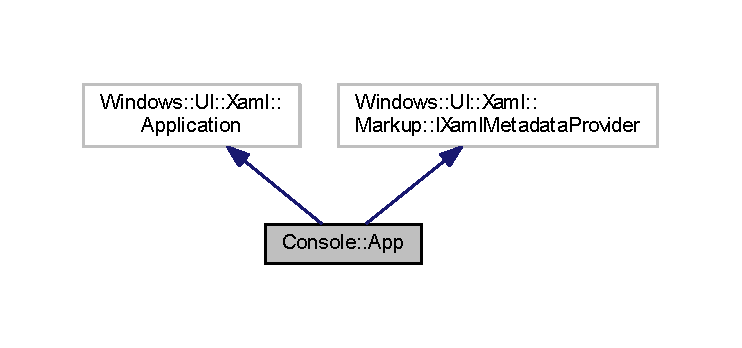
\includegraphics[width=350pt]{class_console_1_1_app__inherit__graph}
\end{center}
\end{figure}


Collaboration diagram for Console\+:\+:App\+:\nopagebreak
\begin{figure}[H]
\begin{center}
\leavevmode
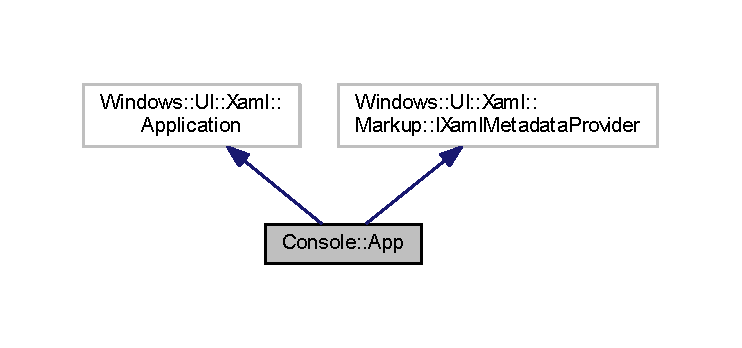
\includegraphics[width=350pt]{class_console_1_1_app__coll__graph}
\end{center}
\end{figure}
\subsection*{Public Member Functions}
\begin{DoxyCompactItemize}
\item 
\mbox{\Hypertarget{class_console_1_1_app_aeaadf4574f8c5b5131ef9d076e4771f2}\label{class_console_1_1_app_aeaadf4574f8c5b5131ef9d076e4771f2}} 
void {\bfseries Initialize\+Component} ()
\item 
\mbox{\Hypertarget{class_console_1_1_app_ab264b34bbb46988b5b66c03705aa27ec}\label{class_console_1_1_app_ab264b34bbb46988b5b66c03705aa27ec}} 
virtual \+::Windows\+::\+U\+I\+::\+Xaml\+::\+Markup\+::\+I\+Xaml\+Type $^\wedge$ {\bfseries Get\+Xaml\+Type} (\+::Windows\+::\+U\+I\+::\+Xaml\+::\+Interop\+::\+Type\+Name type)
\item 
\mbox{\Hypertarget{class_console_1_1_app_ab3e42f369ce3625ca5c88be3364761cb}\label{class_console_1_1_app_ab3e42f369ce3625ca5c88be3364761cb}} 
virtual \+::Windows\+::\+U\+I\+::\+Xaml\+::\+Markup\+::\+I\+Xaml\+Type $^\wedge$ {\bfseries Get\+Xaml\+Type} (\+::Platform\+::\+String$^\wedge$ full\+Name)
\item 
\mbox{\Hypertarget{class_console_1_1_app_a9ff31ca8f383ec11f15e945999ef285e}\label{class_console_1_1_app_a9ff31ca8f383ec11f15e945999ef285e}} 
virtual \+::Platform\+::\+Array$<$\+::Windows\+::\+U\+I\+::\+Xaml\+::\+Markup\+::\+Xmlns\+Definition $>$ $^\wedge$ {\bfseries Get\+Xmlns\+Definitions} ()
\end{DoxyCompactItemize}
\subsection*{Protected Member Functions}
\begin{DoxyCompactItemize}
\item 
\mbox{\Hypertarget{class_console_1_1_app_a850b50800225e29269fa01831d1af441}\label{class_console_1_1_app_a850b50800225e29269fa01831d1af441}} 
virtual void {\bfseries On\+Launched} (Windows\+::\+Application\+Model\+::\+Activation\+::\+Launch\+Activated\+Event\+Args$^\wedge$ aop\+Arg) override
\end{DoxyCompactItemize}


\subsection{Detailed Description}
Provides application-\/specific behavior to supplement the default Application class. 



Definition at line 15 of file App.\+xaml.\+h.



The documentation for this class was generated from the following files\+:\begin{DoxyCompactItemize}
\item 
C\+:/\+Projects/\+Bergermeister\+Home/\+Console/App.\+xaml.\+h\item 
C\+:/\+Projects/\+Bergermeister\+Home/\+Console/\+Generated Files/App.\+g.\+h\item 
C\+:/\+Projects/\+Bergermeister\+Home/\+Console/App.\+xaml.\+cpp\end{DoxyCompactItemize}

\hypertarget{class_thermostat_1_1_app}{}\section{Thermostat\+:\+:App Class Reference}
\label{class_thermostat_1_1_app}\index{Thermostat\+::\+App@{Thermostat\+::\+App}}


Provides application-\/specific behavior to supplement the default Application class.  




{\ttfamily \#include $<$App.\+xaml.\+h$>$}



Inheritance diagram for Thermostat\+:\+:App\+:\nopagebreak
\begin{figure}[H]
\begin{center}
\leavevmode
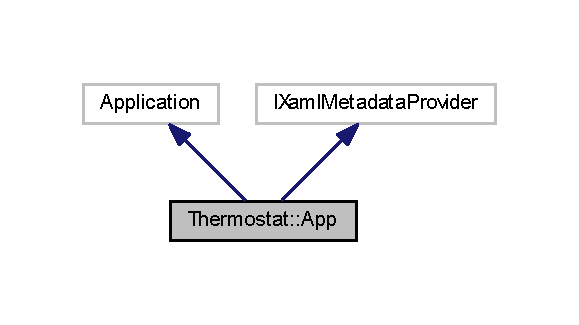
\includegraphics[width=278pt]{class_thermostat_1_1_app__inherit__graph}
\end{center}
\end{figure}


Collaboration diagram for Thermostat\+:\+:App\+:\nopagebreak
\begin{figure}[H]
\begin{center}
\leavevmode
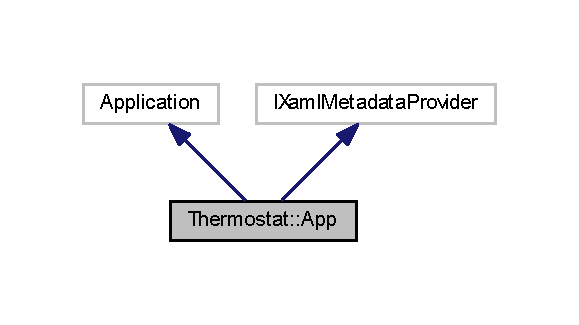
\includegraphics[width=278pt]{class_thermostat_1_1_app__coll__graph}
\end{center}
\end{figure}
\subsection*{Public Member Functions}
\begin{DoxyCompactItemize}
\item 
\mbox{\Hypertarget{class_thermostat_1_1_app_a26e0b25473421b761342a923058f8e65}\label{class_thermostat_1_1_app_a26e0b25473421b761342a923058f8e65}} 
void {\bfseries Initialize\+Component} ()
\item 
\mbox{\Hypertarget{class_thermostat_1_1_app_a7ab270c3097106aa1798e8cad45a064d}\label{class_thermostat_1_1_app_a7ab270c3097106aa1798e8cad45a064d}} 
virtual \+::Windows\+::\+U\+I\+::\+Xaml\+::\+Markup\+::\+I\+Xaml\+Type $^\wedge$ {\bfseries Get\+Xaml\+Type} (\+::Windows\+::\+U\+I\+::\+Xaml\+::\+Interop\+::\+Type\+Name type)
\item 
\mbox{\Hypertarget{class_thermostat_1_1_app_aa919a5c939140144a2c8d56a6613f49d}\label{class_thermostat_1_1_app_aa919a5c939140144a2c8d56a6613f49d}} 
virtual \+::Windows\+::\+U\+I\+::\+Xaml\+::\+Markup\+::\+I\+Xaml\+Type $^\wedge$ {\bfseries Get\+Xaml\+Type} (\+::Platform\+::\+String$^\wedge$ full\+Name)
\item 
\mbox{\Hypertarget{class_thermostat_1_1_app_a8af94ffafa76c0c8fecf82cd45e009bf}\label{class_thermostat_1_1_app_a8af94ffafa76c0c8fecf82cd45e009bf}} 
virtual \+::Platform\+::\+Array$<$\+::Windows\+::\+U\+I\+::\+Xaml\+::\+Markup\+::\+Xmlns\+Definition $>$ $^\wedge$ {\bfseries Get\+Xmlns\+Definitions} ()
\end{DoxyCompactItemize}
\subsection*{Protected Member Functions}
\begin{DoxyCompactItemize}
\item 
virtual void \mbox{\hyperlink{class_thermostat_1_1_app_adffebc0581348c6095a509dc8b1726e7}{On\+Launched}} (Windows\+::\+Application\+Model\+::\+Activation\+::\+Launch\+Activated\+Event\+Args$^\wedge$ e) override
\begin{DoxyCompactList}\small\item\em Invoked when the application is launched normally by the end user. Other entry points will be used such as when the application is launched to open a specific file. \end{DoxyCompactList}\end{DoxyCompactItemize}


\subsection{Detailed Description}
Provides application-\/specific behavior to supplement the default Application class. 



Definition at line 15 of file App.\+xaml.\+h.



\subsection{Member Function Documentation}
\mbox{\Hypertarget{class_thermostat_1_1_app_adffebc0581348c6095a509dc8b1726e7}\label{class_thermostat_1_1_app_adffebc0581348c6095a509dc8b1726e7}} 
\index{Thermostat\+::\+App@{Thermostat\+::\+App}!On\+Launched@{On\+Launched}}
\index{On\+Launched@{On\+Launched}!Thermostat\+::\+App@{Thermostat\+::\+App}}
\subsubsection{\texorpdfstring{On\+Launched()}{OnLaunched()}}
{\footnotesize\ttfamily void App\+::\+On\+Launched (\begin{DoxyParamCaption}\item[{Windows\+::\+Application\+Model\+::\+Activation\+::\+Launch\+Activated\+Event\+Args$^\wedge$}]{e }\end{DoxyParamCaption})\hspace{0.3cm}{\ttfamily [override]}, {\ttfamily [protected]}, {\ttfamily [virtual]}}



Invoked when the application is launched normally by the end user. Other entry points will be used such as when the application is launched to open a specific file. 


\begin{DoxyParams}{Parameters}
{\em e} & Details about the launch request and process.\\
\hline
\end{DoxyParams}


Definition at line 40 of file App.\+xaml.\+cpp.



The documentation for this class was generated from the following files\+:\begin{DoxyCompactItemize}
\item 
C\+:/\+Projects/\+Bergermeister\+Home/\+Thermostat/App.\+xaml.\+h\item 
C\+:/\+Projects/\+Bergermeister\+Home/\+Thermostat/\+Generated Files/App.\+g.\+h\item 
C\+:/\+Projects/\+Bergermeister\+Home/\+Thermostat/App.\+xaml.\+cpp\item 
C\+:/\+Projects/\+Bergermeister\+Home/\+Thermostat/\+Generated Files/App.\+g.\+hpp\end{DoxyCompactItemize}

\hypertarget{class_g_n_common_1_1_g_tc_alert}{}\section{G\+N\+Common\+:\+:G\+Tc\+Alert Class Reference}
\label{class_g_n_common_1_1_g_tc_alert}\index{G\+N\+Common\+::\+G\+Tc\+Alert@{G\+N\+Common\+::\+G\+Tc\+Alert}}


{\ttfamily \#include $<$Alert.\+h$>$}



Collaboration diagram for G\+N\+Common\+:\+:G\+Tc\+Alert\+:\nopagebreak
\begin{figure}[H]
\begin{center}
\leavevmode
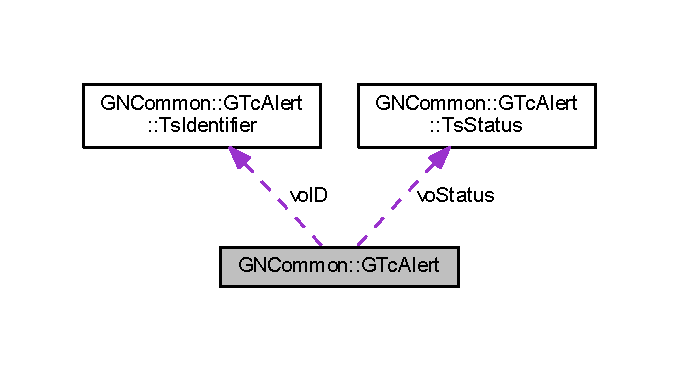
\includegraphics[width=326pt]{class_g_n_common_1_1_g_tc_alert__coll__graph}
\end{center}
\end{figure}
\subsection*{Classes}
\begin{DoxyCompactItemize}
\item 
struct \mbox{\hyperlink{struct_g_n_common_1_1_g_tc_alert_1_1_ts_identifier}{Ts\+Identifier}}
\item 
struct \mbox{\hyperlink{struct_g_n_common_1_1_g_tc_alert_1_1_ts_status}{Ts\+Status}}
\end{DoxyCompactItemize}
\subsection*{Public Types}
\begin{DoxyCompactItemize}
\item 
enum \mbox{\hyperlink{class_g_n_common_1_1_g_tc_alert_a9ef9363f62aae79a7323005ab126507e}{Te\+Level}} \{ \mbox{\hyperlink{class_g_n_common_1_1_g_tc_alert_a9ef9363f62aae79a7323005ab126507eae3bf0642bc4457afb752f6f41a507d86}{Xe\+Level\+None}} = 0, 
\mbox{\hyperlink{class_g_n_common_1_1_g_tc_alert_a9ef9363f62aae79a7323005ab126507eacebd57948648fe7897a9f0e5bb091b31}{Xe\+Level\+Notice}} = 1, 
\mbox{\hyperlink{class_g_n_common_1_1_g_tc_alert_a9ef9363f62aae79a7323005ab126507eaf9a9623077a914bb1b9fc28183670765}{Xe\+Level\+Warning}} = 2, 
\mbox{\hyperlink{class_g_n_common_1_1_g_tc_alert_a9ef9363f62aae79a7323005ab126507ea7a378abd7d3362d4e0677adb5af49bbf}{Xe\+Level\+Alarm}} = 3
 \}
\item 
enum \mbox{\hyperlink{class_g_n_common_1_1_g_tc_alert_aec0a7908321c01ae225df4908d7f3fa0}{Te\+Component}} \{ \mbox{\hyperlink{class_g_n_common_1_1_g_tc_alert_aec0a7908321c01ae225df4908d7f3fa0ab675dd902eb07ebb108c78de28abfc00}{Xe\+Component\+None}} = 0, 
\mbox{\hyperlink{class_g_n_common_1_1_g_tc_alert_aec0a7908321c01ae225df4908d7f3fa0a03e5a94b7c7c39ffa6b7461800a2fa7a}{Xe\+Component\+Server}} = 1, 
\mbox{\hyperlink{class_g_n_common_1_1_g_tc_alert_aec0a7908321c01ae225df4908d7f3fa0a6966d846ba577a7db9225222b7b57235}{Xe\+Component\+Sensor}} = 2
 \}
\item 
enum \mbox{\hyperlink{class_g_n_common_1_1_g_tc_alert_a2deb7f82fcf5d88b4e10d74fa6c28cb7}{Te\+Group}} \{ \mbox{\hyperlink{class_g_n_common_1_1_g_tc_alert_a2deb7f82fcf5d88b4e10d74fa6c28cb7a8c11493234d6ebc2d5654bbbc738be92}{Xe\+Group\+None}} = 0, 
\mbox{\hyperlink{class_g_n_common_1_1_g_tc_alert_a2deb7f82fcf5d88b4e10d74fa6c28cb7a51d90a061a469018e2d235d5919a3ab9}{Xe\+Group\+Network}} = 1
 \}
\end{DoxyCompactItemize}
\subsection*{Public Member Functions}
\begin{DoxyCompactItemize}
\item 
\mbox{\hyperlink{class_g_n_common_1_1_g_tc_alert_ab4874dff7fccf2444439e7e5e4304125}{G\+Tc\+Alert}} (void)
\item 
\mbox{\hyperlink{class_g_n_common_1_1_g_tc_alert_a90f33fbcc71ed945ab1a0dee83bd3ccc}{G\+Tc\+Alert}} (const \mbox{\hyperlink{class_g_n_common_1_1_g_tc_alert}{G\+Tc\+Alert}} \&aor\+Alert)
\item 
\mbox{\hyperlink{class_g_n_common_1_1_g_tc_alert}{G\+Tc\+Alert}} \& \mbox{\hyperlink{class_g_n_common_1_1_g_tc_alert_aba9a3373bd29884b049dfc525f655e5c}{operator=}} (const \mbox{\hyperlink{class_g_n_common_1_1_g_tc_alert}{G\+Tc\+Alert}} \&aor\+Alert)
\item 
\mbox{\hyperlink{class_g_n_common_1_1_g_tc_alert_ad222cd054ec90b1aa8bf6e58e09d608b}{$\sim$\+G\+Tc\+Alert}} (void)
\item 
void \mbox{\hyperlink{class_g_n_common_1_1_g_tc_alert_acbb3761e5ca1af6896c20933be06255f}{M\+Set\+Identifier}} (const \mbox{\hyperlink{struct_g_n_common_1_1_g_tc_alert_1_1_ts_identifier}{Ts\+Identifier}} \&aor\+ID)
\item 
void \mbox{\hyperlink{class_g_n_common_1_1_g_tc_alert_a6e5a7e686b2e78573337c18a49f8d421}{M\+Set\+Status}} (const \mbox{\hyperlink{struct_g_n_common_1_1_g_tc_alert_1_1_ts_status}{Ts\+Status}} \&aor\+Status)
\item 
void \mbox{\hyperlink{class_g_n_common_1_1_g_tc_alert_aca52809ad95713c5ad550cf5d1fc51fa}{M\+Set\+Timestamp}} (const \mbox{\hyperlink{namespace_g_n_common_a01e8527dabf7ab4f123156b0701945eb}{G\+Tu64}} aul\+Timestamp)
\item 
void \mbox{\hyperlink{class_g_n_common_1_1_g_tc_alert_a04f768514f3e12f95e3a6887b02c0576}{M\+Set\+Data}} (const \mbox{\hyperlink{namespace_g_n_common_a01e8527dabf7ab4f123156b0701945eb}{G\+Tu64}} aul\+Trigger)
\item 
\mbox{\hyperlink{struct_g_n_common_1_1_g_tc_alert_1_1_ts_identifier}{Ts\+Identifier}} \mbox{\hyperlink{class_g_n_common_1_1_g_tc_alert_a0baa69459d87c780b3bad22883f29dec}{M\+Get\+Identifier}} (void) const
\item 
\mbox{\hyperlink{struct_g_n_common_1_1_g_tc_alert_1_1_ts_status}{Ts\+Status}} \mbox{\hyperlink{class_g_n_common_1_1_g_tc_alert_a8f37913185860432ccdd65dea58ffe37}{M\+Get\+Status}} (void) const
\item 
\mbox{\hyperlink{namespace_g_n_common_a01e8527dabf7ab4f123156b0701945eb}{G\+Tu64}} \mbox{\hyperlink{class_g_n_common_1_1_g_tc_alert_ae00bea560ef82ed36c4b741d92bd27e6}{M\+Get\+Timestamp}} (void) const
\item 
\mbox{\hyperlink{namespace_g_n_common_a01e8527dabf7ab4f123156b0701945eb}{G\+Tu64}} \mbox{\hyperlink{class_g_n_common_1_1_g_tc_alert_a9e582dccb2205b74923c5d93d787811e}{M\+Get\+Trigger}} (void) const
\end{DoxyCompactItemize}
\subsection*{Static Public Attributes}
\begin{DoxyCompactItemize}
\item 
static const \mbox{\hyperlink{namespace_g_n_common_ae5485474bc8f23e462e920a17b377b53}{G\+Tu32}} \mbox{\hyperlink{class_g_n_common_1_1_g_tc_alert_a17e549148a2f549495b0e8567f546e81}{Xui\+Size\+Of\+Identifier}} = sizeof( \mbox{\hyperlink{struct_g_n_common_1_1_g_tc_alert_1_1_ts_identifier}{Ts\+Identifier}} )
\item 
static const \mbox{\hyperlink{namespace_g_n_common_ae5485474bc8f23e462e920a17b377b53}{G\+Tu32}} \mbox{\hyperlink{class_g_n_common_1_1_g_tc_alert_a8d30391ac04c117ef5e25b9a0fa693e5}{Xui\+Size\+Of\+Status}} = sizeof( \mbox{\hyperlink{struct_g_n_common_1_1_g_tc_alert_1_1_ts_status}{Ts\+Status}} )
\end{DoxyCompactItemize}
\subsection*{Protected Attributes}
\begin{DoxyCompactItemize}
\item 
\mbox{\hyperlink{struct_g_n_common_1_1_g_tc_alert_1_1_ts_identifier}{Ts\+Identifier}} \mbox{\hyperlink{class_g_n_common_1_1_g_tc_alert_a1a54c1bf2758812609e876b9eec75df5}{vo\+ID}}
\item 
\mbox{\hyperlink{struct_g_n_common_1_1_g_tc_alert_1_1_ts_status}{Ts\+Status}} \mbox{\hyperlink{class_g_n_common_1_1_g_tc_alert_a88ffecd8070f3a63f4cd4f677adc43b1}{vo\+Status}}
\item 
\mbox{\hyperlink{namespace_g_n_common_a01e8527dabf7ab4f123156b0701945eb}{G\+Tu64}} \mbox{\hyperlink{class_g_n_common_1_1_g_tc_alert_acc753824948e4d169e7af7083ced87a0}{vul\+Timestamp}}
\item 
\mbox{\hyperlink{namespace_g_n_common_a01e8527dabf7ab4f123156b0701945eb}{G\+Tu64}} \mbox{\hyperlink{class_g_n_common_1_1_g_tc_alert_a125041e4424d1f43c332e980a5f2aaa2}{vul\+Data}}
\end{DoxyCompactItemize}


\subsection{Detailed Description}
Alert Class 

Definition at line 16 of file Alert.\+h.



\subsection{Member Enumeration Documentation}
\mbox{\Hypertarget{class_g_n_common_1_1_g_tc_alert_aec0a7908321c01ae225df4908d7f3fa0}\label{class_g_n_common_1_1_g_tc_alert_aec0a7908321c01ae225df4908d7f3fa0}} 
\index{G\+N\+Common\+::\+G\+Tc\+Alert@{G\+N\+Common\+::\+G\+Tc\+Alert}!Te\+Component@{Te\+Component}}
\index{Te\+Component@{Te\+Component}!G\+N\+Common\+::\+G\+Tc\+Alert@{G\+N\+Common\+::\+G\+Tc\+Alert}}
\subsubsection{\texorpdfstring{Te\+Component}{TeComponent}}
{\footnotesize\ttfamily enum \mbox{\hyperlink{class_g_n_common_1_1_g_tc_alert_aec0a7908321c01ae225df4908d7f3fa0}{G\+N\+Common\+::\+G\+Tc\+Alert\+::\+Te\+Component}}}

\begin{DoxyEnumFields}{Enumerator}
\raisebox{\heightof{T}}[0pt][0pt]{\index{Xe\+Component\+None@{Xe\+Component\+None}!G\+N\+Common\+::\+G\+Tc\+Alert@{G\+N\+Common\+::\+G\+Tc\+Alert}}\index{G\+N\+Common\+::\+G\+Tc\+Alert@{G\+N\+Common\+::\+G\+Tc\+Alert}!Xe\+Component\+None@{Xe\+Component\+None}}}\mbox{\Hypertarget{class_g_n_common_1_1_g_tc_alert_aec0a7908321c01ae225df4908d7f3fa0ab675dd902eb07ebb108c78de28abfc00}\label{class_g_n_common_1_1_g_tc_alert_aec0a7908321c01ae225df4908d7f3fa0ab675dd902eb07ebb108c78de28abfc00}} 
Xe\+Component\+None&Enumerated Component\+: None \\
\hline

\raisebox{\heightof{T}}[0pt][0pt]{\index{Xe\+Component\+Server@{Xe\+Component\+Server}!G\+N\+Common\+::\+G\+Tc\+Alert@{G\+N\+Common\+::\+G\+Tc\+Alert}}\index{G\+N\+Common\+::\+G\+Tc\+Alert@{G\+N\+Common\+::\+G\+Tc\+Alert}!Xe\+Component\+Server@{Xe\+Component\+Server}}}\mbox{\Hypertarget{class_g_n_common_1_1_g_tc_alert_aec0a7908321c01ae225df4908d7f3fa0a03e5a94b7c7c39ffa6b7461800a2fa7a}\label{class_g_n_common_1_1_g_tc_alert_aec0a7908321c01ae225df4908d7f3fa0a03e5a94b7c7c39ffa6b7461800a2fa7a}} 
Xe\+Component\+Server&Enumerated Component\+: Server \\
\hline

\raisebox{\heightof{T}}[0pt][0pt]{\index{Xe\+Component\+Sensor@{Xe\+Component\+Sensor}!G\+N\+Common\+::\+G\+Tc\+Alert@{G\+N\+Common\+::\+G\+Tc\+Alert}}\index{G\+N\+Common\+::\+G\+Tc\+Alert@{G\+N\+Common\+::\+G\+Tc\+Alert}!Xe\+Component\+Sensor@{Xe\+Component\+Sensor}}}\mbox{\Hypertarget{class_g_n_common_1_1_g_tc_alert_aec0a7908321c01ae225df4908d7f3fa0a6966d846ba577a7db9225222b7b57235}\label{class_g_n_common_1_1_g_tc_alert_aec0a7908321c01ae225df4908d7f3fa0a6966d846ba577a7db9225222b7b57235}} 
Xe\+Component\+Sensor&Enumerated Component\+: Sensor \\
\hline

\end{DoxyEnumFields}


Definition at line 33 of file Alert.\+h.

\mbox{\Hypertarget{class_g_n_common_1_1_g_tc_alert_a2deb7f82fcf5d88b4e10d74fa6c28cb7}\label{class_g_n_common_1_1_g_tc_alert_a2deb7f82fcf5d88b4e10d74fa6c28cb7}} 
\index{G\+N\+Common\+::\+G\+Tc\+Alert@{G\+N\+Common\+::\+G\+Tc\+Alert}!Te\+Group@{Te\+Group}}
\index{Te\+Group@{Te\+Group}!G\+N\+Common\+::\+G\+Tc\+Alert@{G\+N\+Common\+::\+G\+Tc\+Alert}}
\subsubsection{\texorpdfstring{Te\+Group}{TeGroup}}
{\footnotesize\ttfamily enum \mbox{\hyperlink{class_g_n_common_1_1_g_tc_alert_a2deb7f82fcf5d88b4e10d74fa6c28cb7}{G\+N\+Common\+::\+G\+Tc\+Alert\+::\+Te\+Group}}}

\begin{DoxyEnumFields}{Enumerator}
\raisebox{\heightof{T}}[0pt][0pt]{\index{Xe\+Group\+None@{Xe\+Group\+None}!G\+N\+Common\+::\+G\+Tc\+Alert@{G\+N\+Common\+::\+G\+Tc\+Alert}}\index{G\+N\+Common\+::\+G\+Tc\+Alert@{G\+N\+Common\+::\+G\+Tc\+Alert}!Xe\+Group\+None@{Xe\+Group\+None}}}\mbox{\Hypertarget{class_g_n_common_1_1_g_tc_alert_a2deb7f82fcf5d88b4e10d74fa6c28cb7a8c11493234d6ebc2d5654bbbc738be92}\label{class_g_n_common_1_1_g_tc_alert_a2deb7f82fcf5d88b4e10d74fa6c28cb7a8c11493234d6ebc2d5654bbbc738be92}} 
Xe\+Group\+None&Enumerated Group\+: None \\
\hline

\raisebox{\heightof{T}}[0pt][0pt]{\index{Xe\+Group\+Network@{Xe\+Group\+Network}!G\+N\+Common\+::\+G\+Tc\+Alert@{G\+N\+Common\+::\+G\+Tc\+Alert}}\index{G\+N\+Common\+::\+G\+Tc\+Alert@{G\+N\+Common\+::\+G\+Tc\+Alert}!Xe\+Group\+Network@{Xe\+Group\+Network}}}\mbox{\Hypertarget{class_g_n_common_1_1_g_tc_alert_a2deb7f82fcf5d88b4e10d74fa6c28cb7a51d90a061a469018e2d235d5919a3ab9}\label{class_g_n_common_1_1_g_tc_alert_a2deb7f82fcf5d88b4e10d74fa6c28cb7a51d90a061a469018e2d235d5919a3ab9}} 
Xe\+Group\+Network&Enumerated Group\+: Network \\
\hline

\end{DoxyEnumFields}


Definition at line 43 of file Alert.\+h.

\mbox{\Hypertarget{class_g_n_common_1_1_g_tc_alert_a9ef9363f62aae79a7323005ab126507e}\label{class_g_n_common_1_1_g_tc_alert_a9ef9363f62aae79a7323005ab126507e}} 
\index{G\+N\+Common\+::\+G\+Tc\+Alert@{G\+N\+Common\+::\+G\+Tc\+Alert}!Te\+Level@{Te\+Level}}
\index{Te\+Level@{Te\+Level}!G\+N\+Common\+::\+G\+Tc\+Alert@{G\+N\+Common\+::\+G\+Tc\+Alert}}
\subsubsection{\texorpdfstring{Te\+Level}{TeLevel}}
{\footnotesize\ttfamily enum \mbox{\hyperlink{class_g_n_common_1_1_g_tc_alert_a9ef9363f62aae79a7323005ab126507e}{G\+N\+Common\+::\+G\+Tc\+Alert\+::\+Te\+Level}}}

\begin{DoxyEnumFields}{Enumerator}
\raisebox{\heightof{T}}[0pt][0pt]{\index{Xe\+Level\+None@{Xe\+Level\+None}!G\+N\+Common\+::\+G\+Tc\+Alert@{G\+N\+Common\+::\+G\+Tc\+Alert}}\index{G\+N\+Common\+::\+G\+Tc\+Alert@{G\+N\+Common\+::\+G\+Tc\+Alert}!Xe\+Level\+None@{Xe\+Level\+None}}}\mbox{\Hypertarget{class_g_n_common_1_1_g_tc_alert_a9ef9363f62aae79a7323005ab126507eae3bf0642bc4457afb752f6f41a507d86}\label{class_g_n_common_1_1_g_tc_alert_a9ef9363f62aae79a7323005ab126507eae3bf0642bc4457afb752f6f41a507d86}} 
Xe\+Level\+None&Enumerated Alert Level\+: None \\
\hline

\raisebox{\heightof{T}}[0pt][0pt]{\index{Xe\+Level\+Notice@{Xe\+Level\+Notice}!G\+N\+Common\+::\+G\+Tc\+Alert@{G\+N\+Common\+::\+G\+Tc\+Alert}}\index{G\+N\+Common\+::\+G\+Tc\+Alert@{G\+N\+Common\+::\+G\+Tc\+Alert}!Xe\+Level\+Notice@{Xe\+Level\+Notice}}}\mbox{\Hypertarget{class_g_n_common_1_1_g_tc_alert_a9ef9363f62aae79a7323005ab126507eacebd57948648fe7897a9f0e5bb091b31}\label{class_g_n_common_1_1_g_tc_alert_a9ef9363f62aae79a7323005ab126507eacebd57948648fe7897a9f0e5bb091b31}} 
Xe\+Level\+Notice&Enumerated Alert Level\+: None \\
\hline

\raisebox{\heightof{T}}[0pt][0pt]{\index{Xe\+Level\+Warning@{Xe\+Level\+Warning}!G\+N\+Common\+::\+G\+Tc\+Alert@{G\+N\+Common\+::\+G\+Tc\+Alert}}\index{G\+N\+Common\+::\+G\+Tc\+Alert@{G\+N\+Common\+::\+G\+Tc\+Alert}!Xe\+Level\+Warning@{Xe\+Level\+Warning}}}\mbox{\Hypertarget{class_g_n_common_1_1_g_tc_alert_a9ef9363f62aae79a7323005ab126507eaf9a9623077a914bb1b9fc28183670765}\label{class_g_n_common_1_1_g_tc_alert_a9ef9363f62aae79a7323005ab126507eaf9a9623077a914bb1b9fc28183670765}} 
Xe\+Level\+Warning&Enumerated Alert Level\+: None \\
\hline

\raisebox{\heightof{T}}[0pt][0pt]{\index{Xe\+Level\+Alarm@{Xe\+Level\+Alarm}!G\+N\+Common\+::\+G\+Tc\+Alert@{G\+N\+Common\+::\+G\+Tc\+Alert}}\index{G\+N\+Common\+::\+G\+Tc\+Alert@{G\+N\+Common\+::\+G\+Tc\+Alert}!Xe\+Level\+Alarm@{Xe\+Level\+Alarm}}}\mbox{\Hypertarget{class_g_n_common_1_1_g_tc_alert_a9ef9363f62aae79a7323005ab126507ea7a378abd7d3362d4e0677adb5af49bbf}\label{class_g_n_common_1_1_g_tc_alert_a9ef9363f62aae79a7323005ab126507ea7a378abd7d3362d4e0677adb5af49bbf}} 
Xe\+Level\+Alarm&Enumerated Alert Level\+: None \\
\hline

\end{DoxyEnumFields}


Definition at line 22 of file Alert.\+h.



\subsection{Constructor \& Destructor Documentation}
\mbox{\Hypertarget{class_g_n_common_1_1_g_tc_alert_ab4874dff7fccf2444439e7e5e4304125}\label{class_g_n_common_1_1_g_tc_alert_ab4874dff7fccf2444439e7e5e4304125}} 
\index{G\+N\+Common\+::\+G\+Tc\+Alert@{G\+N\+Common\+::\+G\+Tc\+Alert}!G\+Tc\+Alert@{G\+Tc\+Alert}}
\index{G\+Tc\+Alert@{G\+Tc\+Alert}!G\+N\+Common\+::\+G\+Tc\+Alert@{G\+N\+Common\+::\+G\+Tc\+Alert}}
\subsubsection{\texorpdfstring{G\+Tc\+Alert()}{GTcAlert()}\hspace{0.1cm}{\footnotesize\ttfamily [1/2]}}
{\footnotesize\ttfamily G\+Tc\+Alert\+::\+G\+Tc\+Alert (\begin{DoxyParamCaption}\item[{void}]{ }\end{DoxyParamCaption})}

Default Constructor 

Definition at line 8 of file Alert.\+cpp.

\mbox{\Hypertarget{class_g_n_common_1_1_g_tc_alert_a90f33fbcc71ed945ab1a0dee83bd3ccc}\label{class_g_n_common_1_1_g_tc_alert_a90f33fbcc71ed945ab1a0dee83bd3ccc}} 
\index{G\+N\+Common\+::\+G\+Tc\+Alert@{G\+N\+Common\+::\+G\+Tc\+Alert}!G\+Tc\+Alert@{G\+Tc\+Alert}}
\index{G\+Tc\+Alert@{G\+Tc\+Alert}!G\+N\+Common\+::\+G\+Tc\+Alert@{G\+N\+Common\+::\+G\+Tc\+Alert}}
\subsubsection{\texorpdfstring{G\+Tc\+Alert()}{GTcAlert()}\hspace{0.1cm}{\footnotesize\ttfamily [2/2]}}
{\footnotesize\ttfamily G\+Tc\+Alert\+::\+G\+Tc\+Alert (\begin{DoxyParamCaption}\item[{const \mbox{\hyperlink{class_g_n_common_1_1_g_tc_alert}{G\+Tc\+Alert}} \&}]{aor\+Alert }\end{DoxyParamCaption})}

Copy Constructor 
\begin{DoxyParams}{Parameters}
{\em aor\+Alert} & Alert Constant Reference to copy \\
\hline
\end{DoxyParams}


Definition at line 32 of file Alert.\+cpp.

\mbox{\Hypertarget{class_g_n_common_1_1_g_tc_alert_ad222cd054ec90b1aa8bf6e58e09d608b}\label{class_g_n_common_1_1_g_tc_alert_ad222cd054ec90b1aa8bf6e58e09d608b}} 
\index{G\+N\+Common\+::\+G\+Tc\+Alert@{G\+N\+Common\+::\+G\+Tc\+Alert}!````~G\+Tc\+Alert@{$\sim$\+G\+Tc\+Alert}}
\index{````~G\+Tc\+Alert@{$\sim$\+G\+Tc\+Alert}!G\+N\+Common\+::\+G\+Tc\+Alert@{G\+N\+Common\+::\+G\+Tc\+Alert}}
\subsubsection{\texorpdfstring{$\sim$\+G\+Tc\+Alert()}{~GTcAlert()}}
{\footnotesize\ttfamily G\+Tc\+Alert\+::$\sim$\+G\+Tc\+Alert (\begin{DoxyParamCaption}\item[{void}]{ }\end{DoxyParamCaption})}

Default Destructor 

Definition at line 67 of file Alert.\+cpp.



\subsection{Member Function Documentation}
\mbox{\Hypertarget{class_g_n_common_1_1_g_tc_alert_a0baa69459d87c780b3bad22883f29dec}\label{class_g_n_common_1_1_g_tc_alert_a0baa69459d87c780b3bad22883f29dec}} 
\index{G\+N\+Common\+::\+G\+Tc\+Alert@{G\+N\+Common\+::\+G\+Tc\+Alert}!M\+Get\+Identifier@{M\+Get\+Identifier}}
\index{M\+Get\+Identifier@{M\+Get\+Identifier}!G\+N\+Common\+::\+G\+Tc\+Alert@{G\+N\+Common\+::\+G\+Tc\+Alert}}
\subsubsection{\texorpdfstring{M\+Get\+Identifier()}{MGetIdentifier()}}
{\footnotesize\ttfamily \mbox{\hyperlink{struct_g_n_common_1_1_g_tc_alert_1_1_ts_identifier}{G\+Tc\+Alert\+::\+Ts\+Identifier}} G\+Tc\+Alert\+::\+M\+Get\+Identifier (\begin{DoxyParamCaption}\item[{void}]{ }\end{DoxyParamCaption}) const}

M\+Get\+Identifier \begin{DoxyReturn}{Returns}
this-\/$>$vo\+ID constant \mbox{\hyperlink{struct_g_n_common_1_1_g_tc_alert_1_1_ts_identifier}{Ts\+Identifier}} 
\end{DoxyReturn}


Definition at line 115 of file Alert.\+cpp.

\mbox{\Hypertarget{class_g_n_common_1_1_g_tc_alert_a8f37913185860432ccdd65dea58ffe37}\label{class_g_n_common_1_1_g_tc_alert_a8f37913185860432ccdd65dea58ffe37}} 
\index{G\+N\+Common\+::\+G\+Tc\+Alert@{G\+N\+Common\+::\+G\+Tc\+Alert}!M\+Get\+Status@{M\+Get\+Status}}
\index{M\+Get\+Status@{M\+Get\+Status}!G\+N\+Common\+::\+G\+Tc\+Alert@{G\+N\+Common\+::\+G\+Tc\+Alert}}
\subsubsection{\texorpdfstring{M\+Get\+Status()}{MGetStatus()}}
{\footnotesize\ttfamily \mbox{\hyperlink{struct_g_n_common_1_1_g_tc_alert_1_1_ts_status}{G\+Tc\+Alert\+::\+Ts\+Status}} G\+Tc\+Alert\+::\+M\+Get\+Status (\begin{DoxyParamCaption}\item[{void}]{ }\end{DoxyParamCaption}) const}

M\+Get\+Status \begin{DoxyReturn}{Returns}
this-\/$>$vo\+Status constant \mbox{\hyperlink{struct_g_n_common_1_1_g_tc_alert_1_1_ts_status}{Ts\+Status}} 
\end{DoxyReturn}


Definition at line 124 of file Alert.\+cpp.

\mbox{\Hypertarget{class_g_n_common_1_1_g_tc_alert_ae00bea560ef82ed36c4b741d92bd27e6}\label{class_g_n_common_1_1_g_tc_alert_ae00bea560ef82ed36c4b741d92bd27e6}} 
\index{G\+N\+Common\+::\+G\+Tc\+Alert@{G\+N\+Common\+::\+G\+Tc\+Alert}!M\+Get\+Timestamp@{M\+Get\+Timestamp}}
\index{M\+Get\+Timestamp@{M\+Get\+Timestamp}!G\+N\+Common\+::\+G\+Tc\+Alert@{G\+N\+Common\+::\+G\+Tc\+Alert}}
\subsubsection{\texorpdfstring{M\+Get\+Timestamp()}{MGetTimestamp()}}
{\footnotesize\ttfamily \mbox{\hyperlink{namespace_g_n_common_a01e8527dabf7ab4f123156b0701945eb}{G\+Tu64}} G\+Tc\+Alert\+::\+M\+Get\+Timestamp (\begin{DoxyParamCaption}\item[{void}]{ }\end{DoxyParamCaption}) const}

M\+Get\+Timestamp \begin{DoxyReturn}{Returns}
this-\/$>$vul\+Timestamp constant 64-\/bit Integer Timestamp 
\end{DoxyReturn}


Definition at line 133 of file Alert.\+cpp.

\mbox{\Hypertarget{class_g_n_common_1_1_g_tc_alert_a9e582dccb2205b74923c5d93d787811e}\label{class_g_n_common_1_1_g_tc_alert_a9e582dccb2205b74923c5d93d787811e}} 
\index{G\+N\+Common\+::\+G\+Tc\+Alert@{G\+N\+Common\+::\+G\+Tc\+Alert}!M\+Get\+Trigger@{M\+Get\+Trigger}}
\index{M\+Get\+Trigger@{M\+Get\+Trigger}!G\+N\+Common\+::\+G\+Tc\+Alert@{G\+N\+Common\+::\+G\+Tc\+Alert}}
\subsubsection{\texorpdfstring{M\+Get\+Trigger()}{MGetTrigger()}}
{\footnotesize\ttfamily \mbox{\hyperlink{namespace_g_n_common_a01e8527dabf7ab4f123156b0701945eb}{G\+Tu64}} G\+Tc\+Alert\+::\+M\+Get\+Trigger (\begin{DoxyParamCaption}\item[{void}]{ }\end{DoxyParamCaption}) const}

M\+Get\+Trigger \begin{DoxyReturn}{Returns}
this-\/$>$vul\+Data constant 64-\/bit Integer Data 
\end{DoxyReturn}


Definition at line 142 of file Alert.\+cpp.

\mbox{\Hypertarget{class_g_n_common_1_1_g_tc_alert_a04f768514f3e12f95e3a6887b02c0576}\label{class_g_n_common_1_1_g_tc_alert_a04f768514f3e12f95e3a6887b02c0576}} 
\index{G\+N\+Common\+::\+G\+Tc\+Alert@{G\+N\+Common\+::\+G\+Tc\+Alert}!M\+Set\+Data@{M\+Set\+Data}}
\index{M\+Set\+Data@{M\+Set\+Data}!G\+N\+Common\+::\+G\+Tc\+Alert@{G\+N\+Common\+::\+G\+Tc\+Alert}}
\subsubsection{\texorpdfstring{M\+Set\+Data()}{MSetData()}}
{\footnotesize\ttfamily void G\+Tc\+Alert\+::\+M\+Set\+Data (\begin{DoxyParamCaption}\item[{const \mbox{\hyperlink{namespace_g_n_common_a01e8527dabf7ab4f123156b0701945eb}{G\+Tu64}}}]{aul\+Data }\end{DoxyParamCaption})}

M\+Set\+Data 
\begin{DoxyParams}{Parameters}
{\em aul\+Data} & constant 64-\/bit Integer Data \\
\hline
\end{DoxyParams}


Definition at line 106 of file Alert.\+cpp.

\mbox{\Hypertarget{class_g_n_common_1_1_g_tc_alert_acbb3761e5ca1af6896c20933be06255f}\label{class_g_n_common_1_1_g_tc_alert_acbb3761e5ca1af6896c20933be06255f}} 
\index{G\+N\+Common\+::\+G\+Tc\+Alert@{G\+N\+Common\+::\+G\+Tc\+Alert}!M\+Set\+Identifier@{M\+Set\+Identifier}}
\index{M\+Set\+Identifier@{M\+Set\+Identifier}!G\+N\+Common\+::\+G\+Tc\+Alert@{G\+N\+Common\+::\+G\+Tc\+Alert}}
\subsubsection{\texorpdfstring{M\+Set\+Identifier()}{MSetIdentifier()}}
{\footnotesize\ttfamily void G\+Tc\+Alert\+::\+M\+Set\+Identifier (\begin{DoxyParamCaption}\item[{const \mbox{\hyperlink{struct_g_n_common_1_1_g_tc_alert_1_1_ts_identifier}{Ts\+Identifier}} \&}]{aor\+ID }\end{DoxyParamCaption})}

M\+Set\+Identifier 
\begin{DoxyParams}{Parameters}
{\em aor\+ID} & \mbox{\hyperlink{struct_identifier}{Identifier}} Structure Constant Reference \\
\hline
\end{DoxyParams}


Definition at line 76 of file Alert.\+cpp.

\mbox{\Hypertarget{class_g_n_common_1_1_g_tc_alert_a6e5a7e686b2e78573337c18a49f8d421}\label{class_g_n_common_1_1_g_tc_alert_a6e5a7e686b2e78573337c18a49f8d421}} 
\index{G\+N\+Common\+::\+G\+Tc\+Alert@{G\+N\+Common\+::\+G\+Tc\+Alert}!M\+Set\+Status@{M\+Set\+Status}}
\index{M\+Set\+Status@{M\+Set\+Status}!G\+N\+Common\+::\+G\+Tc\+Alert@{G\+N\+Common\+::\+G\+Tc\+Alert}}
\subsubsection{\texorpdfstring{M\+Set\+Status()}{MSetStatus()}}
{\footnotesize\ttfamily void G\+Tc\+Alert\+::\+M\+Set\+Status (\begin{DoxyParamCaption}\item[{const \mbox{\hyperlink{struct_g_n_common_1_1_g_tc_alert_1_1_ts_status}{Ts\+Status}} \&}]{aor\+Status }\end{DoxyParamCaption})}

M\+Set\+Status 
\begin{DoxyParams}{Parameters}
{\em aor\+Status} & \mbox{\hyperlink{struct_status}{Status}} Structure Constant Reference \\
\hline
\end{DoxyParams}


Definition at line 88 of file Alert.\+cpp.

\mbox{\Hypertarget{class_g_n_common_1_1_g_tc_alert_aca52809ad95713c5ad550cf5d1fc51fa}\label{class_g_n_common_1_1_g_tc_alert_aca52809ad95713c5ad550cf5d1fc51fa}} 
\index{G\+N\+Common\+::\+G\+Tc\+Alert@{G\+N\+Common\+::\+G\+Tc\+Alert}!M\+Set\+Timestamp@{M\+Set\+Timestamp}}
\index{M\+Set\+Timestamp@{M\+Set\+Timestamp}!G\+N\+Common\+::\+G\+Tc\+Alert@{G\+N\+Common\+::\+G\+Tc\+Alert}}
\subsubsection{\texorpdfstring{M\+Set\+Timestamp()}{MSetTimestamp()}}
{\footnotesize\ttfamily void G\+Tc\+Alert\+::\+M\+Set\+Timestamp (\begin{DoxyParamCaption}\item[{const \mbox{\hyperlink{namespace_g_n_common_a01e8527dabf7ab4f123156b0701945eb}{G\+Tu64}}}]{aul\+Timestamp }\end{DoxyParamCaption})}

M\+Set\+Time\+Stamp 
\begin{DoxyParams}{Parameters}
{\em aul\+Timestamp} & constant 64-\/bit Integer Timestamp \\
\hline
\end{DoxyParams}


Definition at line 97 of file Alert.\+cpp.

\mbox{\Hypertarget{class_g_n_common_1_1_g_tc_alert_aba9a3373bd29884b049dfc525f655e5c}\label{class_g_n_common_1_1_g_tc_alert_aba9a3373bd29884b049dfc525f655e5c}} 
\index{G\+N\+Common\+::\+G\+Tc\+Alert@{G\+N\+Common\+::\+G\+Tc\+Alert}!operator=@{operator=}}
\index{operator=@{operator=}!G\+N\+Common\+::\+G\+Tc\+Alert@{G\+N\+Common\+::\+G\+Tc\+Alert}}
\subsubsection{\texorpdfstring{operator=()}{operator=()}}
{\footnotesize\ttfamily \mbox{\hyperlink{class_g_n_common_1_1_g_tc_alert}{G\+Tc\+Alert}} \& G\+Tc\+Alert\+::operator= (\begin{DoxyParamCaption}\item[{const \mbox{\hyperlink{class_g_n_common_1_1_g_tc_alert}{G\+Tc\+Alert}} \&}]{aor\+Alert }\end{DoxyParamCaption})}

operator= Override 
\begin{DoxyParams}{Parameters}
{\em aor\+Alert} & Alert Constant Reference to copy \\
\hline
\end{DoxyParams}
\begin{DoxyReturn}{Returns}
$\ast$this \mbox{\hyperlink{class_g_n_common_1_1_g_tc_alert}{G\+Tc\+Alert}} Reference 
\end{DoxyReturn}


Definition at line 42 of file Alert.\+cpp.



\subsection{Member Data Documentation}
\mbox{\Hypertarget{class_g_n_common_1_1_g_tc_alert_a1a54c1bf2758812609e876b9eec75df5}\label{class_g_n_common_1_1_g_tc_alert_a1a54c1bf2758812609e876b9eec75df5}} 
\index{G\+N\+Common\+::\+G\+Tc\+Alert@{G\+N\+Common\+::\+G\+Tc\+Alert}!vo\+ID@{vo\+ID}}
\index{vo\+ID@{vo\+ID}!G\+N\+Common\+::\+G\+Tc\+Alert@{G\+N\+Common\+::\+G\+Tc\+Alert}}
\subsubsection{\texorpdfstring{vo\+ID}{voID}}
{\footnotesize\ttfamily \mbox{\hyperlink{struct_g_n_common_1_1_g_tc_alert_1_1_ts_identifier}{Ts\+Identifier}} G\+N\+Common\+::\+G\+Tc\+Alert\+::vo\+ID\hspace{0.3cm}{\ttfamily [protected]}}

Encoded \mbox{\hyperlink{struct_identifier}{Identifier}} 

Definition at line 79 of file Alert.\+h.

\mbox{\Hypertarget{class_g_n_common_1_1_g_tc_alert_a88ffecd8070f3a63f4cd4f677adc43b1}\label{class_g_n_common_1_1_g_tc_alert_a88ffecd8070f3a63f4cd4f677adc43b1}} 
\index{G\+N\+Common\+::\+G\+Tc\+Alert@{G\+N\+Common\+::\+G\+Tc\+Alert}!vo\+Status@{vo\+Status}}
\index{vo\+Status@{vo\+Status}!G\+N\+Common\+::\+G\+Tc\+Alert@{G\+N\+Common\+::\+G\+Tc\+Alert}}
\subsubsection{\texorpdfstring{vo\+Status}{voStatus}}
{\footnotesize\ttfamily \mbox{\hyperlink{struct_g_n_common_1_1_g_tc_alert_1_1_ts_status}{Ts\+Status}} G\+N\+Common\+::\+G\+Tc\+Alert\+::vo\+Status\hspace{0.3cm}{\ttfamily [protected]}}

Encoded \mbox{\hyperlink{struct_status}{Status}} 

Definition at line 80 of file Alert.\+h.

\mbox{\Hypertarget{class_g_n_common_1_1_g_tc_alert_a125041e4424d1f43c332e980a5f2aaa2}\label{class_g_n_common_1_1_g_tc_alert_a125041e4424d1f43c332e980a5f2aaa2}} 
\index{G\+N\+Common\+::\+G\+Tc\+Alert@{G\+N\+Common\+::\+G\+Tc\+Alert}!vul\+Data@{vul\+Data}}
\index{vul\+Data@{vul\+Data}!G\+N\+Common\+::\+G\+Tc\+Alert@{G\+N\+Common\+::\+G\+Tc\+Alert}}
\subsubsection{\texorpdfstring{vul\+Data}{vulData}}
{\footnotesize\ttfamily \mbox{\hyperlink{namespace_g_n_common_a01e8527dabf7ab4f123156b0701945eb}{G\+Tu64}} G\+N\+Common\+::\+G\+Tc\+Alert\+::vul\+Data\hspace{0.3cm}{\ttfamily [protected]}}

64-\/bit Additional Data 

Definition at line 82 of file Alert.\+h.

\mbox{\Hypertarget{class_g_n_common_1_1_g_tc_alert_acc753824948e4d169e7af7083ced87a0}\label{class_g_n_common_1_1_g_tc_alert_acc753824948e4d169e7af7083ced87a0}} 
\index{G\+N\+Common\+::\+G\+Tc\+Alert@{G\+N\+Common\+::\+G\+Tc\+Alert}!vul\+Timestamp@{vul\+Timestamp}}
\index{vul\+Timestamp@{vul\+Timestamp}!G\+N\+Common\+::\+G\+Tc\+Alert@{G\+N\+Common\+::\+G\+Tc\+Alert}}
\subsubsection{\texorpdfstring{vul\+Timestamp}{vulTimestamp}}
{\footnotesize\ttfamily \mbox{\hyperlink{namespace_g_n_common_a01e8527dabf7ab4f123156b0701945eb}{G\+Tu64}} G\+N\+Common\+::\+G\+Tc\+Alert\+::vul\+Timestamp\hspace{0.3cm}{\ttfamily [protected]}}

64-\/bit Timestamp of Occurrence 

Definition at line 81 of file Alert.\+h.

\mbox{\Hypertarget{class_g_n_common_1_1_g_tc_alert_a17e549148a2f549495b0e8567f546e81}\label{class_g_n_common_1_1_g_tc_alert_a17e549148a2f549495b0e8567f546e81}} 
\index{G\+N\+Common\+::\+G\+Tc\+Alert@{G\+N\+Common\+::\+G\+Tc\+Alert}!Xui\+Size\+Of\+Identifier@{Xui\+Size\+Of\+Identifier}}
\index{Xui\+Size\+Of\+Identifier@{Xui\+Size\+Of\+Identifier}!G\+N\+Common\+::\+G\+Tc\+Alert@{G\+N\+Common\+::\+G\+Tc\+Alert}}
\subsubsection{\texorpdfstring{Xui\+Size\+Of\+Identifier}{XuiSizeOfIdentifier}}
{\footnotesize\ttfamily const \mbox{\hyperlink{namespace_g_n_common_ae5485474bc8f23e462e920a17b377b53}{G\+Tu32}} G\+N\+Common\+::\+G\+Tc\+Alert\+::\+Xui\+Size\+Of\+Identifier = sizeof( \mbox{\hyperlink{struct_g_n_common_1_1_g_tc_alert_1_1_ts_identifier}{Ts\+Identifier}} )\hspace{0.3cm}{\ttfamily [static]}}

Size of \mbox{\hyperlink{struct_identifier}{Identifier}} 

Definition at line 75 of file Alert.\+h.

\mbox{\Hypertarget{class_g_n_common_1_1_g_tc_alert_a8d30391ac04c117ef5e25b9a0fa693e5}\label{class_g_n_common_1_1_g_tc_alert_a8d30391ac04c117ef5e25b9a0fa693e5}} 
\index{G\+N\+Common\+::\+G\+Tc\+Alert@{G\+N\+Common\+::\+G\+Tc\+Alert}!Xui\+Size\+Of\+Status@{Xui\+Size\+Of\+Status}}
\index{Xui\+Size\+Of\+Status@{Xui\+Size\+Of\+Status}!G\+N\+Common\+::\+G\+Tc\+Alert@{G\+N\+Common\+::\+G\+Tc\+Alert}}
\subsubsection{\texorpdfstring{Xui\+Size\+Of\+Status}{XuiSizeOfStatus}}
{\footnotesize\ttfamily const \mbox{\hyperlink{namespace_g_n_common_ae5485474bc8f23e462e920a17b377b53}{G\+Tu32}} G\+N\+Common\+::\+G\+Tc\+Alert\+::\+Xui\+Size\+Of\+Status = sizeof( \mbox{\hyperlink{struct_g_n_common_1_1_g_tc_alert_1_1_ts_status}{Ts\+Status}} )\hspace{0.3cm}{\ttfamily [static]}}

Size of \mbox{\hyperlink{struct_status}{Status}} 

Definition at line 76 of file Alert.\+h.



The documentation for this class was generated from the following files\+:\begin{DoxyCompactItemize}
\item 
C\+:/\+Projects/\+Bergermeister\+Home/\+Common/\+Source/\mbox{\hyperlink{_alert_8h}{Alert.\+h}}\item 
C\+:/\+Projects/\+Bergermeister\+Home/\+Common/\+Source/Alert.\+cpp\end{DoxyCompactItemize}

\hypertarget{class_g_n_common_1_1_g_n_drivers_1_1_g_tc_d_h_t_sensor}{}\section{G\+N\+Common\+:\+:G\+N\+Drivers\+:\+:G\+Tc\+D\+H\+T\+Sensor Class Reference}
\label{class_g_n_common_1_1_g_n_drivers_1_1_g_tc_d_h_t_sensor}\index{G\+N\+Common\+::\+G\+N\+Drivers\+::\+G\+Tc\+D\+H\+T\+Sensor@{G\+N\+Common\+::\+G\+N\+Drivers\+::\+G\+Tc\+D\+H\+T\+Sensor}}


Collaboration diagram for G\+N\+Common\+:\+:G\+N\+Drivers\+:\+:G\+Tc\+D\+H\+T\+Sensor\+:\nopagebreak
\begin{figure}[H]
\begin{center}
\leavevmode
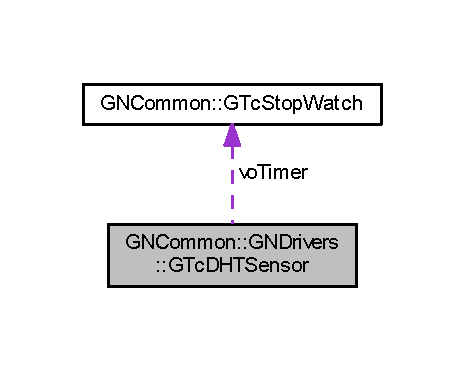
\includegraphics[width=223pt]{class_g_n_common_1_1_g_n_drivers_1_1_g_tc_d_h_t_sensor__coll__graph}
\end{center}
\end{figure}
\subsection*{Public Types}
\begin{DoxyCompactItemize}
\item 
\mbox{\Hypertarget{class_g_n_common_1_1_g_n_drivers_1_1_g_tc_d_h_t_sensor_a7bf14575ba24e0bc8b085c3249b68930}\label{class_g_n_common_1_1_g_n_drivers_1_1_g_tc_d_h_t_sensor_a7bf14575ba24e0bc8b085c3249b68930}} 
enum {\bfseries Te\+Status} \{ \newline
{\bfseries Qe\+Status\+None} = 0, 
{\bfseries Qe\+Status\+Timeout}, 
{\bfseries Qe\+Status\+Missing\+Data}, 
{\bfseries Qe\+Status\+Invalid\+Data}, 
\newline
{\bfseries Qe\+Status\+Success}, 
{\bfseries Qe\+Status\+None} = 0, 
{\bfseries Qe\+Status\+Start\+High}, 
{\bfseries Qe\+Status\+Start\+Low}, 
\newline
{\bfseries Qe\+Status\+Timeout}, 
{\bfseries Qe\+Status\+Missing\+Data}, 
{\bfseries Qe\+Status\+Invalid\+Data}, 
{\bfseries Qe\+Status\+Success}
 \}
\item 
\mbox{\Hypertarget{class_g_n_common_1_1_g_n_drivers_1_1_g_tc_d_h_t_sensor_a7bf14575ba24e0bc8b085c3249b68930}\label{class_g_n_common_1_1_g_n_drivers_1_1_g_tc_d_h_t_sensor_a7bf14575ba24e0bc8b085c3249b68930}} 
enum {\bfseries Te\+Status} \{ \newline
{\bfseries Qe\+Status\+None} = 0, 
{\bfseries Qe\+Status\+Timeout}, 
{\bfseries Qe\+Status\+Missing\+Data}, 
{\bfseries Qe\+Status\+Invalid\+Data}, 
\newline
{\bfseries Qe\+Status\+Success}, 
{\bfseries Qe\+Status\+None} = 0, 
{\bfseries Qe\+Status\+Start\+High}, 
{\bfseries Qe\+Status\+Start\+Low}, 
\newline
{\bfseries Qe\+Status\+Timeout}, 
{\bfseries Qe\+Status\+Missing\+Data}, 
{\bfseries Qe\+Status\+Invalid\+Data}, 
{\bfseries Qe\+Status\+Success}
 \}
\end{DoxyCompactItemize}
\subsection*{Public Member Functions}
\begin{DoxyCompactItemize}
\item 
\mbox{\Hypertarget{class_g_n_common_1_1_g_n_drivers_1_1_g_tc_d_h_t_sensor_a28a32f003a0916d1009564d0dedf75de}\label{class_g_n_common_1_1_g_n_drivers_1_1_g_tc_d_h_t_sensor_a28a32f003a0916d1009564d0dedf75de}} 
{\bfseries G\+Tc\+D\+H\+T\+Sensor} (const \mbox{\hyperlink{class_g_n_common_1_1_g_n_drivers_1_1_g_tc_d_h_t_sensor}{G\+Tc\+D\+H\+T\+Sensor}} \&aor\+Sensor)
\item 
\mbox{\Hypertarget{class_g_n_common_1_1_g_n_drivers_1_1_g_tc_d_h_t_sensor_a42e5b9edaea5dcfc2c914a25ba41b1ef}\label{class_g_n_common_1_1_g_n_drivers_1_1_g_tc_d_h_t_sensor_a42e5b9edaea5dcfc2c914a25ba41b1ef}} 
\mbox{\hyperlink{class_g_n_common_1_1_g_n_drivers_1_1_g_tc_d_h_t_sensor}{G\+Tc\+D\+H\+T\+Sensor}} \& {\bfseries operator=} (const \mbox{\hyperlink{class_g_n_common_1_1_g_n_drivers_1_1_g_tc_d_h_t_sensor}{G\+Tc\+D\+H\+T\+Sensor}} \&aor\+Sensor)
\item 
\mbox{\Hypertarget{class_g_n_common_1_1_g_n_drivers_1_1_g_tc_d_h_t_sensor_a66a5d9d2f43f1a42dce542181d98acb5}\label{class_g_n_common_1_1_g_n_drivers_1_1_g_tc_d_h_t_sensor_a66a5d9d2f43f1a42dce542181d98acb5}} 
void {\bfseries M\+Initialize} (Windows\+::\+Devices\+::\+Gpio\+::\+Gpio\+Pin$^\wedge$ aop\+Pin)
\item 
\mbox{\Hypertarget{class_g_n_common_1_1_g_n_drivers_1_1_g_tc_d_h_t_sensor_af433fb954e3f8c8b5ed2c794d1be2563}\label{class_g_n_common_1_1_g_n_drivers_1_1_g_tc_d_h_t_sensor_af433fb954e3f8c8b5ed2c794d1be2563}} 
Te\+Status {\bfseries M\+Sample} (void)
\item 
\mbox{\Hypertarget{class_g_n_common_1_1_g_n_drivers_1_1_g_tc_d_h_t_sensor_a6a29ed7188a817c4e35a8d87ee34d65c}\label{class_g_n_common_1_1_g_n_drivers_1_1_g_tc_d_h_t_sensor_a6a29ed7188a817c4e35a8d87ee34d65c}} 
\mbox{\hyperlink{namespace_g_n_common_a6b5283329f609e2175dd0c91fc1520ba}{G\+N\+Common\+::\+G\+Tb8}} {\bfseries M\+Pull\+Resistor\+Required} (void) const
\item 
\mbox{\Hypertarget{class_g_n_common_1_1_g_n_drivers_1_1_g_tc_d_h_t_sensor_aedc75ca476023f30adfc10cf27e431cd}\label{class_g_n_common_1_1_g_n_drivers_1_1_g_tc_d_h_t_sensor_aedc75ca476023f30adfc10cf27e431cd}} 
\mbox{\hyperlink{namespace_g_n_common_a6b5283329f609e2175dd0c91fc1520ba}{G\+N\+Common\+::\+G\+Tb8}} {\bfseries M\+Is\+Valid} (void) const
\item 
\mbox{\Hypertarget{class_g_n_common_1_1_g_n_drivers_1_1_g_tc_d_h_t_sensor_a17d7fe7d6cd82e388b48c2653a95077d}\label{class_g_n_common_1_1_g_n_drivers_1_1_g_tc_d_h_t_sensor_a17d7fe7d6cd82e388b48c2653a95077d}} 
\mbox{\hyperlink{namespace_g_n_common_a22b37ff753b3e7a48d9d31addf35a739}{G\+N\+Common\+::\+G\+Tf64}} {\bfseries M\+Humidity} (void) const
\item 
\mbox{\Hypertarget{class_g_n_common_1_1_g_n_drivers_1_1_g_tc_d_h_t_sensor_a717cd7d8fe381f24edcb3fa69436b0fb}\label{class_g_n_common_1_1_g_n_drivers_1_1_g_tc_d_h_t_sensor_a717cd7d8fe381f24edcb3fa69436b0fb}} 
\mbox{\hyperlink{namespace_g_n_common_a22b37ff753b3e7a48d9d31addf35a739}{G\+N\+Common\+::\+G\+Tf64}} {\bfseries M\+Temperature} (void) const
\item 
\mbox{\Hypertarget{class_g_n_common_1_1_g_n_drivers_1_1_g_tc_d_h_t_sensor_a25970d3c8f5b697e69d4743bb77959bb}\label{class_g_n_common_1_1_g_n_drivers_1_1_g_tc_d_h_t_sensor_a25970d3c8f5b697e69d4743bb77959bb}} 
{\bfseries G\+Tc\+D\+H\+T\+Sensor} (const \mbox{\hyperlink{class_g_n_common_1_1_g_n_drivers_1_1_g_tc_d_h_t_sensor}{G\+Tc\+D\+H\+T\+Sensor}} \&aor\+Sensor)
\item 
\mbox{\Hypertarget{class_g_n_common_1_1_g_n_drivers_1_1_g_tc_d_h_t_sensor_a04e6eac312290dfebf94e12b512b52f9}\label{class_g_n_common_1_1_g_n_drivers_1_1_g_tc_d_h_t_sensor_a04e6eac312290dfebf94e12b512b52f9}} 
\mbox{\hyperlink{class_g_n_common_1_1_g_n_drivers_1_1_g_tc_d_h_t_sensor}{G\+Tc\+D\+H\+T\+Sensor}} \& {\bfseries operator=} (const \mbox{\hyperlink{class_g_n_common_1_1_g_n_drivers_1_1_g_tc_d_h_t_sensor}{G\+Tc\+D\+H\+T\+Sensor}} \&aor\+Sensor)
\item 
\mbox{\Hypertarget{class_g_n_common_1_1_g_n_drivers_1_1_g_tc_d_h_t_sensor_aa8012ed0e167335873c6da1a14e77bac}\label{class_g_n_common_1_1_g_n_drivers_1_1_g_tc_d_h_t_sensor_aa8012ed0e167335873c6da1a14e77bac}} 
void {\bfseries M\+Initialize} (Windows\+::\+Devices\+::\+Gpio\+::\+Gpio\+Pin$^\wedge$ aop\+Pin)
\item 
\mbox{\Hypertarget{class_g_n_common_1_1_g_n_drivers_1_1_g_tc_d_h_t_sensor_afdf34c8b2a22b5e782af77d269675881}\label{class_g_n_common_1_1_g_n_drivers_1_1_g_tc_d_h_t_sensor_afdf34c8b2a22b5e782af77d269675881}} 
Te\+Status {\bfseries M\+Sample} (void)
\item 
\mbox{\Hypertarget{class_g_n_common_1_1_g_n_drivers_1_1_g_tc_d_h_t_sensor_a4293c991280004b758b907b8426eaf92}\label{class_g_n_common_1_1_g_n_drivers_1_1_g_tc_d_h_t_sensor_a4293c991280004b758b907b8426eaf92}} 
\mbox{\hyperlink{namespace_g_n_common_a6b5283329f609e2175dd0c91fc1520ba}{G\+N\+Common\+::\+G\+Tb8}} {\bfseries M\+Pull\+Resistor\+Required} (void) const
\item 
\mbox{\Hypertarget{class_g_n_common_1_1_g_n_drivers_1_1_g_tc_d_h_t_sensor_aa7f53cce05c35eb81133659caa23325b}\label{class_g_n_common_1_1_g_n_drivers_1_1_g_tc_d_h_t_sensor_aa7f53cce05c35eb81133659caa23325b}} 
\mbox{\hyperlink{namespace_g_n_common_a6b5283329f609e2175dd0c91fc1520ba}{G\+N\+Common\+::\+G\+Tb8}} {\bfseries M\+Is\+Valid} (void) const
\item 
\mbox{\Hypertarget{class_g_n_common_1_1_g_n_drivers_1_1_g_tc_d_h_t_sensor_afaba4e1a0d3e9a9d848c20a90256b2e5}\label{class_g_n_common_1_1_g_n_drivers_1_1_g_tc_d_h_t_sensor_afaba4e1a0d3e9a9d848c20a90256b2e5}} 
\mbox{\hyperlink{namespace_g_n_common_a22b37ff753b3e7a48d9d31addf35a739}{G\+N\+Common\+::\+G\+Tf64}} {\bfseries M\+Humidity} (void) const
\item 
\mbox{\Hypertarget{class_g_n_common_1_1_g_n_drivers_1_1_g_tc_d_h_t_sensor_a122f70a816b339247e2ee8ea88e3fe89}\label{class_g_n_common_1_1_g_n_drivers_1_1_g_tc_d_h_t_sensor_a122f70a816b339247e2ee8ea88e3fe89}} 
\mbox{\hyperlink{namespace_g_n_common_a22b37ff753b3e7a48d9d31addf35a739}{G\+N\+Common\+::\+G\+Tf64}} {\bfseries M\+Temperature} (void) const
\end{DoxyCompactItemize}
\subsection*{Protected Member Functions}
\begin{DoxyCompactItemize}
\item 
\mbox{\Hypertarget{class_g_n_common_1_1_g_n_drivers_1_1_g_tc_d_h_t_sensor_a9fe2b4dde94b5d9c8ecd5a21cc73c928}\label{class_g_n_common_1_1_g_n_drivers_1_1_g_tc_d_h_t_sensor_a9fe2b4dde94b5d9c8ecd5a21cc73c928}} 
void {\bfseries m\+Sleep} (\mbox{\hyperlink{namespace_g_n_common_a01e8527dabf7ab4f123156b0701945eb}{G\+N\+Common\+::\+G\+Tu64}} aul\+Microseconds)
\item 
\mbox{\Hypertarget{class_g_n_common_1_1_g_n_drivers_1_1_g_tc_d_h_t_sensor_a27065c9d674768053ef47549c2671993}\label{class_g_n_common_1_1_g_n_drivers_1_1_g_tc_d_h_t_sensor_a27065c9d674768053ef47549c2671993}} 
\mbox{\hyperlink{namespace_g_n_common_ae5485474bc8f23e462e920a17b377b53}{G\+Tu32}} {\bfseries m\+Check\+Pulse} (Windows\+::\+Devices\+::\+Gpio\+::\+Gpio\+Pin\+Value ke\+Level)
\end{DoxyCompactItemize}
\subsection*{Protected Attributes}
\begin{DoxyCompactItemize}
\item 
\mbox{\Hypertarget{class_g_n_common_1_1_g_n_drivers_1_1_g_tc_d_h_t_sensor_add75ea9fe9710905cd21f853ba256375}\label{class_g_n_common_1_1_g_n_drivers_1_1_g_tc_d_h_t_sensor_add75ea9fe9710905cd21f853ba256375}} 
Windows\+::\+Devices\+::\+Gpio\+::\+Gpio\+Pin $^\wedge$ {\bfseries vop\+Pin}
\item 
\mbox{\Hypertarget{class_g_n_common_1_1_g_n_drivers_1_1_g_tc_d_h_t_sensor_af94fdbd8a41443d69d20198ca8436add}\label{class_g_n_common_1_1_g_n_drivers_1_1_g_tc_d_h_t_sensor_af94fdbd8a41443d69d20198ca8436add}} 
Windows\+::\+Devices\+::\+Gpio\+::\+Gpio\+Pin\+Drive\+Mode {\bfseries ve\+Input\+Drive\+Mode}
\item 
\mbox{\Hypertarget{class_g_n_common_1_1_g_n_drivers_1_1_g_tc_d_h_t_sensor_a5cf37517afea9493b10cf746b01fc505}\label{class_g_n_common_1_1_g_n_drivers_1_1_g_tc_d_h_t_sensor_a5cf37517afea9493b10cf746b01fc505}} 
std\+::bitset$<$ 40 $>$ {\bfseries vo\+Bits}
\item 
\mbox{\Hypertarget{class_g_n_common_1_1_g_n_drivers_1_1_g_tc_d_h_t_sensor_abdeb7fea8d6c886c75f3a73213f57c37}\label{class_g_n_common_1_1_g_n_drivers_1_1_g_tc_d_h_t_sensor_abdeb7fea8d6c886c75f3a73213f57c37}} 
\mbox{\hyperlink{namespace_g_n_common_a551fbbb7c62c00956ef69d960ca9ccc3}{G\+Tu8}} {\bfseries vuc\+Data} \mbox{[}xui\+Byte\+Count\mbox{]}
\item 
\mbox{\Hypertarget{class_g_n_common_1_1_g_n_drivers_1_1_g_tc_d_h_t_sensor_a94be04c4acbc94b4ba7280fd6a9756bd}\label{class_g_n_common_1_1_g_n_drivers_1_1_g_tc_d_h_t_sensor_a94be04c4acbc94b4ba7280fd6a9756bd}} 
\mbox{\hyperlink{class_g_n_common_1_1_g_tc_stop_watch}{G\+N\+Common\+::\+G\+Tc\+Stop\+Watch}} {\bfseries vo\+Timer}
\end{DoxyCompactItemize}
\subsection*{Static Protected Attributes}
\begin{DoxyCompactItemize}
\item 
\mbox{\Hypertarget{class_g_n_common_1_1_g_n_drivers_1_1_g_tc_d_h_t_sensor_a6ed915985319f53bb24e7daf4b15e818}\label{class_g_n_common_1_1_g_n_drivers_1_1_g_tc_d_h_t_sensor_a6ed915985319f53bb24e7daf4b15e818}} 
static const \mbox{\hyperlink{namespace_g_n_common_a01e8527dabf7ab4f123156b0701945eb}{G\+Tu64}} {\bfseries xul\+Threshold} = 110\+LL
\item 
\mbox{\Hypertarget{class_g_n_common_1_1_g_n_drivers_1_1_g_tc_d_h_t_sensor_a723b978a24a1326fef1078921cd37771}\label{class_g_n_common_1_1_g_n_drivers_1_1_g_tc_d_h_t_sensor_a723b978a24a1326fef1078921cd37771}} 
static const \mbox{\hyperlink{namespace_g_n_common_a01e8527dabf7ab4f123156b0701945eb}{G\+Tu64}} {\bfseries xul\+Micros} = 1000000\+LL
\item 
\mbox{\Hypertarget{class_g_n_common_1_1_g_n_drivers_1_1_g_tc_d_h_t_sensor_ae3a47859593e45963dc33438465e6eb0}\label{class_g_n_common_1_1_g_n_drivers_1_1_g_tc_d_h_t_sensor_ae3a47859593e45963dc33438465e6eb0}} 
static const \mbox{\hyperlink{namespace_g_n_common_ae5485474bc8f23e462e920a17b377b53}{G\+Tu32}} {\bfseries xui\+Sample\+Hold\+Low\+Millis} = 18
\item 
\mbox{\Hypertarget{class_g_n_common_1_1_g_n_drivers_1_1_g_tc_d_h_t_sensor_aa986ef9126846c33bf675e66db6f1668}\label{class_g_n_common_1_1_g_n_drivers_1_1_g_tc_d_h_t_sensor_aa986ef9126846c33bf675e66db6f1668}} 
static const \mbox{\hyperlink{namespace_g_n_common_a01e8527dabf7ab4f123156b0701945eb}{G\+Tu64}} {\bfseries xul\+Timeout\+Edge} = 1
\item 
\mbox{\Hypertarget{class_g_n_common_1_1_g_n_drivers_1_1_g_tc_d_h_t_sensor_ae8e1fe75e34556116a3d0717ebfcf9dd}\label{class_g_n_common_1_1_g_n_drivers_1_1_g_tc_d_h_t_sensor_ae8e1fe75e34556116a3d0717ebfcf9dd}} 
static const \mbox{\hyperlink{namespace_g_n_common_a01e8527dabf7ab4f123156b0701945eb}{G\+Tu64}} {\bfseries xul\+Timeout\+Sample} = 10
\item 
\mbox{\Hypertarget{class_g_n_common_1_1_g_n_drivers_1_1_g_tc_d_h_t_sensor_a7be983a722a7341e12c7ec71c687869c}\label{class_g_n_common_1_1_g_n_drivers_1_1_g_tc_d_h_t_sensor_a7be983a722a7341e12c7ec71c687869c}} 
static const \mbox{\hyperlink{namespace_g_n_common_a01e8527dabf7ab4f123156b0701945eb}{G\+N\+Common\+::\+G\+Tu64}} {\bfseries xul\+Threshold} = 110\+LL
\item 
\mbox{\Hypertarget{class_g_n_common_1_1_g_n_drivers_1_1_g_tc_d_h_t_sensor_aa41a24c57e1fbb39f06c38aa7b07412d}\label{class_g_n_common_1_1_g_n_drivers_1_1_g_tc_d_h_t_sensor_aa41a24c57e1fbb39f06c38aa7b07412d}} 
static const \mbox{\hyperlink{namespace_g_n_common_a01e8527dabf7ab4f123156b0701945eb}{G\+N\+Common\+::\+G\+Tu64}} {\bfseries xul\+Micros} = 1000000\+LL
\item 
\mbox{\Hypertarget{class_g_n_common_1_1_g_n_drivers_1_1_g_tc_d_h_t_sensor_ab81aca8e6f299e7a6c3a9ca06253e199}\label{class_g_n_common_1_1_g_n_drivers_1_1_g_tc_d_h_t_sensor_ab81aca8e6f299e7a6c3a9ca06253e199}} 
static const \mbox{\hyperlink{namespace_g_n_common_ae5485474bc8f23e462e920a17b377b53}{G\+N\+Common\+::\+G\+Tu32}} {\bfseries xui\+Delay\+Hold\+Low} = 20
\item 
\mbox{\Hypertarget{class_g_n_common_1_1_g_n_drivers_1_1_g_tc_d_h_t_sensor_ad3c0df855aa3ba780c2f97a4d402496f}\label{class_g_n_common_1_1_g_n_drivers_1_1_g_tc_d_h_t_sensor_ad3c0df855aa3ba780c2f97a4d402496f}} 
static const \mbox{\hyperlink{namespace_g_n_common_ae5485474bc8f23e462e920a17b377b53}{G\+N\+Common\+::\+G\+Tu32}} {\bfseries xui\+Delay\+Hold\+High} = 40
\item 
\mbox{\Hypertarget{class_g_n_common_1_1_g_n_drivers_1_1_g_tc_d_h_t_sensor_a47848280212bc6c73d522e213e43e691}\label{class_g_n_common_1_1_g_n_drivers_1_1_g_tc_d_h_t_sensor_a47848280212bc6c73d522e213e43e691}} 
static const \mbox{\hyperlink{namespace_g_n_common_ae5485474bc8f23e462e920a17b377b53}{G\+N\+Common\+::\+G\+Tu32}} {\bfseries xui\+Delay\+Poll} = 80
\item 
\mbox{\Hypertarget{class_g_n_common_1_1_g_n_drivers_1_1_g_tc_d_h_t_sensor_a85170bca155444455fecc6c7153b1583}\label{class_g_n_common_1_1_g_n_drivers_1_1_g_tc_d_h_t_sensor_a85170bca155444455fecc6c7153b1583}} 
static const \mbox{\hyperlink{namespace_g_n_common_ae5485474bc8f23e462e920a17b377b53}{G\+N\+Common\+::\+G\+Tu32}} {\bfseries xui\+Delay\+Read} = 30
\item 
\mbox{\Hypertarget{class_g_n_common_1_1_g_n_drivers_1_1_g_tc_d_h_t_sensor_a099467ee5206d950d7c329c3f54cbbbe}\label{class_g_n_common_1_1_g_n_drivers_1_1_g_tc_d_h_t_sensor_a099467ee5206d950d7c329c3f54cbbbe}} 
static const \mbox{\hyperlink{namespace_g_n_common_a01e8527dabf7ab4f123156b0701945eb}{G\+N\+Common\+::\+G\+Tu64}} {\bfseries xui\+Timeout} = 1000
\item 
\mbox{\Hypertarget{class_g_n_common_1_1_g_n_drivers_1_1_g_tc_d_h_t_sensor_aa6c646fd5dfc1613c97dabc1b86ea4b8}\label{class_g_n_common_1_1_g_n_drivers_1_1_g_tc_d_h_t_sensor_aa6c646fd5dfc1613c97dabc1b86ea4b8}} 
static const \mbox{\hyperlink{namespace_g_n_common_a01e8527dabf7ab4f123156b0701945eb}{G\+N\+Common\+::\+G\+Tu64}} {\bfseries xul\+Timeout\+Edge} = 1
\item 
\mbox{\Hypertarget{class_g_n_common_1_1_g_n_drivers_1_1_g_tc_d_h_t_sensor_a90e9a1dd52460d5c90503f057267b87d}\label{class_g_n_common_1_1_g_n_drivers_1_1_g_tc_d_h_t_sensor_a90e9a1dd52460d5c90503f057267b87d}} 
static const \mbox{\hyperlink{namespace_g_n_common_a01e8527dabf7ab4f123156b0701945eb}{G\+N\+Common\+::\+G\+Tu64}} {\bfseries xul\+Timeout\+Sample} = 10
\item 
\mbox{\Hypertarget{class_g_n_common_1_1_g_n_drivers_1_1_g_tc_d_h_t_sensor_a697bb711acabf32ba3b7e55befc1a142}\label{class_g_n_common_1_1_g_n_drivers_1_1_g_tc_d_h_t_sensor_a697bb711acabf32ba3b7e55befc1a142}} 
static const \mbox{\hyperlink{namespace_g_n_common_ae5485474bc8f23e462e920a17b377b53}{G\+N\+Common\+::\+G\+Tu32}} {\bfseries xui\+Byte\+Count} = 5
\end{DoxyCompactItemize}


\subsection{Detailed Description}


Definition at line 11 of file D\+H\+T\+Sensor.\+h.



The documentation for this class was generated from the following files\+:\begin{DoxyCompactItemize}
\item 
C\+:/\+Projects/\+Bergermeister\+Home/\+Common/\+Source/\+Drivers-\/bak/D\+H\+T\+Sensor.\+h\item 
C\+:/\+Projects/\+Bergermeister\+Home/\+Common/\+Source/\+Drivers-\/bak/D\+H\+T\+Sensor.\+cpp\end{DoxyCompactItemize}

\hypertarget{class_console_1_1_g_tc_d_h_t_sensor}{}\section{Console\+:\+:G\+Tc\+D\+H\+T\+Sensor Class Reference}
\label{class_console_1_1_g_tc_d_h_t_sensor}\index{Console\+::\+G\+Tc\+D\+H\+T\+Sensor@{Console\+::\+G\+Tc\+D\+H\+T\+Sensor}}
\subsection*{Public Types}
\begin{DoxyCompactItemize}
\item 
\mbox{\Hypertarget{class_console_1_1_g_tc_d_h_t_sensor_a773cdd4c7af39e023dbc893f07f6ad32}\label{class_console_1_1_g_tc_d_h_t_sensor_a773cdd4c7af39e023dbc893f07f6ad32}} 
enum {\bfseries Te\+Status} \{ \newline
{\bfseries Qe\+Status\+None} = 0, 
{\bfseries Qe\+Status\+Timeout}, 
{\bfseries Qe\+Status\+Missing\+Data}, 
{\bfseries Qe\+Status\+Invalid\+Data}, 
\newline
{\bfseries Qe\+Status\+Success}
 \}
\end{DoxyCompactItemize}
\subsection*{Public Member Functions}
\begin{DoxyCompactItemize}
\item 
\mbox{\Hypertarget{class_console_1_1_g_tc_d_h_t_sensor_a28a32f003a0916d1009564d0dedf75de}\label{class_console_1_1_g_tc_d_h_t_sensor_a28a32f003a0916d1009564d0dedf75de}} 
{\bfseries G\+Tc\+D\+H\+T\+Sensor} (const \mbox{\hyperlink{class_console_1_1_g_tc_d_h_t_sensor}{G\+Tc\+D\+H\+T\+Sensor}} \&aor\+Sensor)
\item 
\mbox{\Hypertarget{class_console_1_1_g_tc_d_h_t_sensor_a42e5b9edaea5dcfc2c914a25ba41b1ef}\label{class_console_1_1_g_tc_d_h_t_sensor_a42e5b9edaea5dcfc2c914a25ba41b1ef}} 
\mbox{\hyperlink{class_console_1_1_g_tc_d_h_t_sensor}{G\+Tc\+D\+H\+T\+Sensor}} \& {\bfseries operator=} (const \mbox{\hyperlink{class_console_1_1_g_tc_d_h_t_sensor}{G\+Tc\+D\+H\+T\+Sensor}} \&aor\+Sensor)
\item 
\mbox{\Hypertarget{class_console_1_1_g_tc_d_h_t_sensor_a66a5d9d2f43f1a42dce542181d98acb5}\label{class_console_1_1_g_tc_d_h_t_sensor_a66a5d9d2f43f1a42dce542181d98acb5}} 
void {\bfseries M\+Initialize} (Windows\+::\+Devices\+::\+Gpio\+::\+Gpio\+Pin$^\wedge$ aop\+Pin)
\item 
\mbox{\Hypertarget{class_console_1_1_g_tc_d_h_t_sensor_af433fb954e3f8c8b5ed2c794d1be2563}\label{class_console_1_1_g_tc_d_h_t_sensor_af433fb954e3f8c8b5ed2c794d1be2563}} 
Te\+Status {\bfseries M\+Sample} (void)
\item 
\mbox{\Hypertarget{class_console_1_1_g_tc_d_h_t_sensor_a6a29ed7188a817c4e35a8d87ee34d65c}\label{class_console_1_1_g_tc_d_h_t_sensor_a6a29ed7188a817c4e35a8d87ee34d65c}} 
\mbox{\hyperlink{namespace_g_n_common_a6b5283329f609e2175dd0c91fc1520ba}{G\+N\+Common\+::\+G\+Tb8}} {\bfseries M\+Pull\+Resistor\+Required} (void) const
\item 
\mbox{\Hypertarget{class_console_1_1_g_tc_d_h_t_sensor_aedc75ca476023f30adfc10cf27e431cd}\label{class_console_1_1_g_tc_d_h_t_sensor_aedc75ca476023f30adfc10cf27e431cd}} 
\mbox{\hyperlink{namespace_g_n_common_a6b5283329f609e2175dd0c91fc1520ba}{G\+N\+Common\+::\+G\+Tb8}} {\bfseries M\+Is\+Valid} (void) const
\item 
\mbox{\Hypertarget{class_console_1_1_g_tc_d_h_t_sensor_a17d7fe7d6cd82e388b48c2653a95077d}\label{class_console_1_1_g_tc_d_h_t_sensor_a17d7fe7d6cd82e388b48c2653a95077d}} 
\mbox{\hyperlink{namespace_g_n_common_a22b37ff753b3e7a48d9d31addf35a739}{G\+N\+Common\+::\+G\+Tf64}} {\bfseries M\+Humidity} (void) const
\item 
\mbox{\Hypertarget{class_console_1_1_g_tc_d_h_t_sensor_a717cd7d8fe381f24edcb3fa69436b0fb}\label{class_console_1_1_g_tc_d_h_t_sensor_a717cd7d8fe381f24edcb3fa69436b0fb}} 
\mbox{\hyperlink{namespace_g_n_common_a22b37ff753b3e7a48d9d31addf35a739}{G\+N\+Common\+::\+G\+Tf64}} {\bfseries M\+Temperature} (void) const
\end{DoxyCompactItemize}
\subsection*{Protected Attributes}
\begin{DoxyCompactItemize}
\item 
\mbox{\Hypertarget{class_console_1_1_g_tc_d_h_t_sensor_ac7dd137b30bbda611805f59ec56a42e8}\label{class_console_1_1_g_tc_d_h_t_sensor_ac7dd137b30bbda611805f59ec56a42e8}} 
Windows\+::\+Devices\+::\+Gpio\+::\+Gpio\+Pin $^\wedge$ {\bfseries vop\+Pin}
\item 
\mbox{\Hypertarget{class_console_1_1_g_tc_d_h_t_sensor_aae9001c25efa86a88f5931a00373d60d}\label{class_console_1_1_g_tc_d_h_t_sensor_aae9001c25efa86a88f5931a00373d60d}} 
Windows\+::\+Devices\+::\+Gpio\+::\+Gpio\+Pin\+Drive\+Mode {\bfseries ve\+Input\+Drive\+Mode}
\item 
\mbox{\Hypertarget{class_console_1_1_g_tc_d_h_t_sensor_aa2a05e14611469c21527ea7bb85d88f6}\label{class_console_1_1_g_tc_d_h_t_sensor_aa2a05e14611469c21527ea7bb85d88f6}} 
std\+::bitset$<$ 40 $>$ {\bfseries vo\+Bits}
\end{DoxyCompactItemize}
\subsection*{Static Protected Attributes}
\begin{DoxyCompactItemize}
\item 
\mbox{\Hypertarget{class_console_1_1_g_tc_d_h_t_sensor_ae039fda43f1f4fcb89f0dcd42a9f8536}\label{class_console_1_1_g_tc_d_h_t_sensor_ae039fda43f1f4fcb89f0dcd42a9f8536}} 
static const \mbox{\hyperlink{namespace_g_n_common_a01e8527dabf7ab4f123156b0701945eb}{G\+N\+Common\+::\+G\+Tu64}} {\bfseries xul\+Threshold} = 110\+LL
\item 
\mbox{\Hypertarget{class_console_1_1_g_tc_d_h_t_sensor_abe17cac05439ef8b1305bf2800b34806}\label{class_console_1_1_g_tc_d_h_t_sensor_abe17cac05439ef8b1305bf2800b34806}} 
static const \mbox{\hyperlink{namespace_g_n_common_a01e8527dabf7ab4f123156b0701945eb}{G\+N\+Common\+::\+G\+Tu64}} {\bfseries xul\+Micros} = 1000000\+LL
\item 
\mbox{\Hypertarget{class_console_1_1_g_tc_d_h_t_sensor_a7817e1d85a7235c9d7cb75cee501a718}\label{class_console_1_1_g_tc_d_h_t_sensor_a7817e1d85a7235c9d7cb75cee501a718}} 
static const \mbox{\hyperlink{namespace_g_n_common_ae5485474bc8f23e462e920a17b377b53}{G\+N\+Common\+::\+G\+Tu32}} {\bfseries xui\+Sample\+Hold\+Low\+Millis} = 18
\item 
\mbox{\Hypertarget{class_console_1_1_g_tc_d_h_t_sensor_a23fdf91d2ac3beef278a969e63bcb91a}\label{class_console_1_1_g_tc_d_h_t_sensor_a23fdf91d2ac3beef278a969e63bcb91a}} 
static const \mbox{\hyperlink{namespace_g_n_common_a01e8527dabf7ab4f123156b0701945eb}{G\+N\+Common\+::\+G\+Tu64}} {\bfseries xul\+Timeout\+Edge} = 1
\item 
\mbox{\Hypertarget{class_console_1_1_g_tc_d_h_t_sensor_a3e60c98618191a61bddfe22791840ad2}\label{class_console_1_1_g_tc_d_h_t_sensor_a3e60c98618191a61bddfe22791840ad2}} 
static const \mbox{\hyperlink{namespace_g_n_common_a01e8527dabf7ab4f123156b0701945eb}{G\+N\+Common\+::\+G\+Tu64}} {\bfseries xul\+Timeout\+Sample} = 10
\end{DoxyCompactItemize}


\subsection{Detailed Description}


Definition at line 7 of file D\+H\+T\+Sensor.\+h.



The documentation for this class was generated from the following files\+:\begin{DoxyCompactItemize}
\item 
C\+:/\+Projects/\+Bergermeister\+Home/\+Console/D\+H\+T\+Sensor.\+h\item 
C\+:/\+Projects/\+Bergermeister\+Home/\+Console/D\+H\+T\+Sensor.\+cpp\end{DoxyCompactItemize}

\hypertarget{class_g_n_common_1_1_g_n_component_1_1_g_tc_event}{}\section{G\+N\+Common\+:\+:G\+N\+Component\+:\+:G\+Tc\+Event$<$ aui\+Max\+Listeners $>$ Class Template Reference}
\label{class_g_n_common_1_1_g_n_component_1_1_g_tc_event}\index{G\+N\+Common\+::\+G\+N\+Component\+::\+G\+Tc\+Event$<$ aui\+Max\+Listeners $>$@{G\+N\+Common\+::\+G\+N\+Component\+::\+G\+Tc\+Event$<$ aui\+Max\+Listeners $>$}}
\subsection*{Public Member Functions}
\begin{DoxyCompactItemize}
\item 
\mbox{\Hypertarget{class_g_n_common_1_1_g_n_component_1_1_g_tc_event_a97e465b1537a3a906f2e1040f60ea880}\label{class_g_n_common_1_1_g_n_component_1_1_g_tc_event_a97e465b1537a3a906f2e1040f60ea880}} 
void {\bfseries M\+Notify} (void $\ast$aop\+Sender, const \mbox{\hyperlink{namespace_g_n_common_a941b527ef318f318aed7903dc832b7e4}{Tu32}} aui\+Identifier)
\item 
\mbox{\Hypertarget{class_g_n_common_1_1_g_n_component_1_1_g_tc_event_adb06bbd1286161d6fda279e96197e961}\label{class_g_n_common_1_1_g_n_component_1_1_g_tc_event_adb06bbd1286161d6fda279e96197e961}} 
\mbox{\hyperlink{class_g_n_common_1_1_g_n_component_1_1_g_tc_event}{G\+Tc\+Event}} \& {\bfseries operator+=} (const \mbox{\hyperlink{class_g_n_common_1_1_g_n_component_1_1_g_tc_listener}{G\+Tc\+Listener}} \&aor\+Listener)
\item 
\mbox{\Hypertarget{class_g_n_common_1_1_g_n_component_1_1_g_tc_event_a901c402621b19c65c16696c6ba5e0a48}\label{class_g_n_common_1_1_g_n_component_1_1_g_tc_event_a901c402621b19c65c16696c6ba5e0a48}} 
\mbox{\hyperlink{class_g_n_common_1_1_g_n_component_1_1_g_tc_event}{G\+Tc\+Event}} \& {\bfseries operator-\/=} (const \mbox{\hyperlink{class_g_n_common_1_1_g_n_component_1_1_g_tc_listener}{G\+Tc\+Listener}} \&aor\+Listener)
\end{DoxyCompactItemize}
\subsection*{Protected Attributes}
\begin{DoxyCompactItemize}
\item 
\mbox{\Hypertarget{class_g_n_common_1_1_g_n_component_1_1_g_tc_event_a2c7fde6aa76e38ce816fbad446b2f3ea}\label{class_g_n_common_1_1_g_n_component_1_1_g_tc_event_a2c7fde6aa76e38ce816fbad446b2f3ea}} 
\mbox{\hyperlink{class_g_n_common_1_1_g_n_containers_1_1_g_tc_list_node}{G\+N\+Common\+::\+G\+N\+Containers\+::\+G\+Tc\+List\+Node}}$<$ \mbox{\hyperlink{class_g_n_common_1_1_g_n_component_1_1_g_tc_listener}{G\+Tc\+Listener}} $>$ {\bfseries vo\+Buffer} \mbox{[}aui\+Max\+Listeners\mbox{]}
\item 
\mbox{\Hypertarget{class_g_n_common_1_1_g_n_component_1_1_g_tc_event_a1158c71b941779b471dd3905737e38f0}\label{class_g_n_common_1_1_g_n_component_1_1_g_tc_event_a1158c71b941779b471dd3905737e38f0}} 
\mbox{\hyperlink{class_g_n_common_1_1_g_n_containers_1_1_g_tc_linked_list}{G\+N\+Common\+::\+G\+N\+Containers\+::\+G\+Tc\+Linked\+List}}$<$ \mbox{\hyperlink{class_g_n_common_1_1_g_n_component_1_1_g_tc_listener}{G\+Tc\+Listener}} $>$ {\bfseries vo\+Listeners}
\end{DoxyCompactItemize}


\subsection{Detailed Description}
\subsubsection*{template$<$Tu32 aui\+Max\+Listeners$>$\newline
class G\+N\+Common\+::\+G\+N\+Component\+::\+G\+Tc\+Event$<$ aui\+Max\+Listeners $>$}



Definition at line \mbox{\hyperlink{_event_8h_source_l00008}{8}} of file \mbox{\hyperlink{_event_8h_source}{Event.\+h}}.



The documentation for this class was generated from the following file\+:\begin{DoxyCompactItemize}
\item 
C\+:/\+Projects/\+Bergermeister\+Home/\+Software/\+Common/inc/\+Component/Event.\+h\end{DoxyCompactItemize}

\hypertarget{class_g_n_common_1_1_g_n_containers_1_1_g_tc_linked_list}{}\section{G\+N\+Common\+:\+:G\+N\+Containers\+:\+:G\+Tc\+Linked\+List$<$ G\+Tc\+Type $>$ Class Template Reference}
\label{class_g_n_common_1_1_g_n_containers_1_1_g_tc_linked_list}\index{G\+N\+Common\+::\+G\+N\+Containers\+::\+G\+Tc\+Linked\+List$<$ G\+Tc\+Type $>$@{G\+N\+Common\+::\+G\+N\+Containers\+::\+G\+Tc\+Linked\+List$<$ G\+Tc\+Type $>$}}
\subsection*{Public Member Functions}
\begin{DoxyCompactItemize}
\item 
\mbox{\Hypertarget{class_g_n_common_1_1_g_n_containers_1_1_g_tc_linked_list_a518200cd19bae250a9ba97924c983bb5}\label{class_g_n_common_1_1_g_n_containers_1_1_g_tc_linked_list_a518200cd19bae250a9ba97924c983bb5}} 
void {\bfseries M\+Initialize} (\mbox{\hyperlink{class_g_n_common_1_1_g_n_containers_1_1_g_tc_list_node}{G\+Tc\+List\+Node}}$<$ G\+Tc\+Type $>$ $\ast$aop\+Buffer, \mbox{\hyperlink{namespace_g_n_common_ae5485474bc8f23e462e920a17b377b53}{G\+Tu32}} aui\+Size)
\item 
\mbox{\Hypertarget{class_g_n_common_1_1_g_n_containers_1_1_g_tc_linked_list_ac8baca8da25b4cc84697491d5958c98b}\label{class_g_n_common_1_1_g_n_containers_1_1_g_tc_linked_list_ac8baca8da25b4cc84697491d5958c98b}} 
\mbox{\hyperlink{namespace_g_n_common_a6b5283329f609e2175dd0c91fc1520ba}{G\+Tb8}} {\bfseries M\+Is\+Initialized} (void) const
\item 
\mbox{\Hypertarget{class_g_n_common_1_1_g_n_containers_1_1_g_tc_linked_list_aa0f6acade55d81941d00d8cb232189f7}\label{class_g_n_common_1_1_g_n_containers_1_1_g_tc_linked_list_aa0f6acade55d81941d00d8cb232189f7}} 
\mbox{\hyperlink{namespace_g_n_common_a6b5283329f609e2175dd0c91fc1520ba}{G\+Tb8}} {\bfseries M\+Insert\+At\+Head} (G\+Tc\+Type \&aor\+Object)
\item 
\mbox{\Hypertarget{class_g_n_common_1_1_g_n_containers_1_1_g_tc_linked_list_a481b86e6615c53a1825de2a21d7ecbca}\label{class_g_n_common_1_1_g_n_containers_1_1_g_tc_linked_list_a481b86e6615c53a1825de2a21d7ecbca}} 
\mbox{\hyperlink{namespace_g_n_common_a6b5283329f609e2175dd0c91fc1520ba}{G\+Tb8}} {\bfseries M\+Insert\+At\+Tail} (G\+Tc\+Type \&aor\+Object)
\item 
\mbox{\Hypertarget{class_g_n_common_1_1_g_n_containers_1_1_g_tc_linked_list_af6146b5588299c553900fec7a66bca76}\label{class_g_n_common_1_1_g_n_containers_1_1_g_tc_linked_list_af6146b5588299c553900fec7a66bca76}} 
\mbox{\hyperlink{namespace_g_n_common_a6b5283329f609e2175dd0c91fc1520ba}{G\+Tb8}} {\bfseries M\+Insert} (G\+Tc\+Type \&aor\+Object)
\item 
\mbox{\Hypertarget{class_g_n_common_1_1_g_n_containers_1_1_g_tc_linked_list_a4eba202327f1b8cff690e27104a2cc07}\label{class_g_n_common_1_1_g_n_containers_1_1_g_tc_linked_list_a4eba202327f1b8cff690e27104a2cc07}} 
\mbox{\hyperlink{namespace_g_n_common_a6b5283329f609e2175dd0c91fc1520ba}{G\+Tb8}} {\bfseries M\+Remove\+Head} (void)
\item 
\mbox{\Hypertarget{class_g_n_common_1_1_g_n_containers_1_1_g_tc_linked_list_a77dbf09ee36ba902db5b1fd96fd0b180}\label{class_g_n_common_1_1_g_n_containers_1_1_g_tc_linked_list_a77dbf09ee36ba902db5b1fd96fd0b180}} 
\mbox{\hyperlink{namespace_g_n_common_a6b5283329f609e2175dd0c91fc1520ba}{G\+Tb8}} {\bfseries M\+Remove\+Tail} (void)
\item 
\mbox{\Hypertarget{class_g_n_common_1_1_g_n_containers_1_1_g_tc_linked_list_a9c668c02719387a6f465732322ee0915}\label{class_g_n_common_1_1_g_n_containers_1_1_g_tc_linked_list_a9c668c02719387a6f465732322ee0915}} 
\mbox{\hyperlink{namespace_g_n_common_a6b5283329f609e2175dd0c91fc1520ba}{G\+Tb8}} {\bfseries M\+Remove} (G\+Tc\+Type \&aor\+Object)
\end{DoxyCompactItemize}
\subsection*{Protected Attributes}
\begin{DoxyCompactItemize}
\item 
\mbox{\Hypertarget{class_g_n_common_1_1_g_n_containers_1_1_g_tc_linked_list_a299d6bb0c04d7baeb08183659e8a5ca9}\label{class_g_n_common_1_1_g_n_containers_1_1_g_tc_linked_list_a299d6bb0c04d7baeb08183659e8a5ca9}} 
\mbox{\hyperlink{class_g_n_common_1_1_g_n_containers_1_1_g_tc_list_node}{G\+Tc\+List\+Node}}$<$ G\+Tc\+Type $>$ $\ast$ {\bfseries vop\+Buff}
\item 
\mbox{\Hypertarget{class_g_n_common_1_1_g_n_containers_1_1_g_tc_linked_list_a5d1acc6861679e509aed31ca6202a50d}\label{class_g_n_common_1_1_g_n_containers_1_1_g_tc_linked_list_a5d1acc6861679e509aed31ca6202a50d}} 
\mbox{\hyperlink{class_g_n_common_1_1_g_n_containers_1_1_g_tc_list_node}{G\+Tc\+List\+Node}}$<$ G\+Tc\+Type $>$ $\ast$ {\bfseries vop\+Head}
\item 
\mbox{\Hypertarget{class_g_n_common_1_1_g_n_containers_1_1_g_tc_linked_list_ad13c0905aaed40122179dc54e6aec08f}\label{class_g_n_common_1_1_g_n_containers_1_1_g_tc_linked_list_ad13c0905aaed40122179dc54e6aec08f}} 
\mbox{\hyperlink{class_g_n_common_1_1_g_n_containers_1_1_g_tc_list_node}{G\+Tc\+List\+Node}}$<$ G\+Tc\+Type $>$ $\ast$ {\bfseries vop\+Tail}
\item 
\mbox{\Hypertarget{class_g_n_common_1_1_g_n_containers_1_1_g_tc_linked_list_ad14313f4f09de3c24c98bc6f7e3bba05}\label{class_g_n_common_1_1_g_n_containers_1_1_g_tc_linked_list_ad14313f4f09de3c24c98bc6f7e3bba05}} 
\mbox{\hyperlink{namespace_g_n_common_ae5485474bc8f23e462e920a17b377b53}{G\+Tu32}} {\bfseries vui\+Size}
\item 
\mbox{\Hypertarget{class_g_n_common_1_1_g_n_containers_1_1_g_tc_linked_list_a19cd7bdd93f5e4abe4cb582707d28975}\label{class_g_n_common_1_1_g_n_containers_1_1_g_tc_linked_list_a19cd7bdd93f5e4abe4cb582707d28975}} 
\mbox{\hyperlink{namespace_g_n_common_ae5485474bc8f23e462e920a17b377b53}{G\+Tu32}} {\bfseries vui\+Count}
\item 
\mbox{\Hypertarget{class_g_n_common_1_1_g_n_containers_1_1_g_tc_linked_list_a2e0e22b42eed50533ac3a08b37166128}\label{class_g_n_common_1_1_g_n_containers_1_1_g_tc_linked_list_a2e0e22b42eed50533ac3a08b37166128}} 
\mbox{\hyperlink{namespace_g_n_common_a6b5283329f609e2175dd0c91fc1520ba}{G\+Tb8}} {\bfseries vb\+Initialized}
\end{DoxyCompactItemize}


\subsection{Detailed Description}
\subsubsection*{template$<$class G\+Tc\+Type$>$\newline
class G\+N\+Common\+::\+G\+N\+Containers\+::\+G\+Tc\+Linked\+List$<$ G\+Tc\+Type $>$}



Definition at line 8 of file Linked\+List.\+h.



The documentation for this class was generated from the following file\+:\begin{DoxyCompactItemize}
\item 
C\+:/\+Projects/\+Bergermeister\+Home/\+Common/\+Source/\+Containers/Linked\+List.\+h\end{DoxyCompactItemize}

\hypertarget{class_g_n_common_1_1_g_n_containers_1_1_g_tc_list}{}\section{G\+N\+Common\+:\+:G\+N\+Containers\+:\+:G\+Tc\+List$<$ G\+Tc\+Type $>$ Class Template Reference}
\label{class_g_n_common_1_1_g_n_containers_1_1_g_tc_list}\index{G\+N\+Common\+::\+G\+N\+Containers\+::\+G\+Tc\+List$<$ G\+Tc\+Type $>$@{G\+N\+Common\+::\+G\+N\+Containers\+::\+G\+Tc\+List$<$ G\+Tc\+Type $>$}}
\subsection*{Public Member Functions}
\begin{DoxyCompactItemize}
\item 
\mbox{\Hypertarget{class_g_n_common_1_1_g_n_containers_1_1_g_tc_list_a4b0299bbadadc6f465d0d4ef28c12307}\label{class_g_n_common_1_1_g_n_containers_1_1_g_tc_list_a4b0299bbadadc6f465d0d4ef28c12307}} 
{\bfseries G\+Tc\+List} (G\+Tc\+Type $\ast$aop\+Buffer, const \mbox{\hyperlink{namespace_g_n_common_a941b527ef318f318aed7903dc832b7e4}{Tu32}} aui\+Capacity)
\item 
\mbox{\Hypertarget{class_g_n_common_1_1_g_n_containers_1_1_g_tc_list_a36e56c7b6659a448750f902a0026acc0}\label{class_g_n_common_1_1_g_n_containers_1_1_g_tc_list_a36e56c7b6659a448750f902a0026acc0}} 
{\bfseries G\+Tc\+List} (const \mbox{\hyperlink{class_g_n_common_1_1_g_n_containers_1_1_g_tc_list}{G\+Tc\+List}}$<$ G\+Tc\+Type $>$ \&aor\+List)
\item 
\mbox{\Hypertarget{class_g_n_common_1_1_g_n_containers_1_1_g_tc_list_a025e8a62abb5e84151e21416c407973b}\label{class_g_n_common_1_1_g_n_containers_1_1_g_tc_list_a025e8a62abb5e84151e21416c407973b}} 
virtual \mbox{\hyperlink{class_g_n_common_1_1_g_n_containers_1_1_g_tc_list}{G\+Tc\+List}}$<$ G\+Tc\+Type $>$ \& {\bfseries operator=} (const \mbox{\hyperlink{class_g_n_common_1_1_g_n_containers_1_1_g_tc_list}{G\+Tc\+List}}$<$ G\+Tc\+Type $>$ \&aor\+List)
\item 
\mbox{\Hypertarget{class_g_n_common_1_1_g_n_containers_1_1_g_tc_list_a2734cc013b1e9016c8563539af6bb038}\label{class_g_n_common_1_1_g_n_containers_1_1_g_tc_list_a2734cc013b1e9016c8563539af6bb038}} 
virtual \mbox{\hyperlink{namespace_g_n_common_a8115dc7ed53b6e5b52e6bfde1632ea74}{Tb8}} {\bfseries M\+Add} (const G\+Tc\+Type \&aor\+Item)
\item 
\mbox{\Hypertarget{class_g_n_common_1_1_g_n_containers_1_1_g_tc_list_a37746ffc76546337b39253004817a037}\label{class_g_n_common_1_1_g_n_containers_1_1_g_tc_list_a37746ffc76546337b39253004817a037}} 
virtual \mbox{\hyperlink{namespace_g_n_common_a8115dc7ed53b6e5b52e6bfde1632ea74}{Tb8}} {\bfseries M\+Insert} (const G\+Tc\+Type \&aor\+Item, const \mbox{\hyperlink{namespace_g_n_common_a941b527ef318f318aed7903dc832b7e4}{Tu32}} aui\+Index)
\item 
\mbox{\Hypertarget{class_g_n_common_1_1_g_n_containers_1_1_g_tc_list_a127e02e2e13760b065f95e9d0f076062}\label{class_g_n_common_1_1_g_n_containers_1_1_g_tc_list_a127e02e2e13760b065f95e9d0f076062}} 
virtual \mbox{\hyperlink{namespace_g_n_common_a8115dc7ed53b6e5b52e6bfde1632ea74}{Tb8}} {\bfseries M\+Remove} (const G\+Tc\+Type \&aor\+Item)
\item 
\mbox{\Hypertarget{class_g_n_common_1_1_g_n_containers_1_1_g_tc_list_ae018f2d4b96ddefbf3640c4a399ca487}\label{class_g_n_common_1_1_g_n_containers_1_1_g_tc_list_ae018f2d4b96ddefbf3640c4a399ca487}} 
virtual \mbox{\hyperlink{namespace_g_n_common_a8115dc7ed53b6e5b52e6bfde1632ea74}{Tb8}} {\bfseries M\+Remvoe\+At} (const \mbox{\hyperlink{namespace_g_n_common_a941b527ef318f318aed7903dc832b7e4}{Tu32}} aui\+Index)
\item 
\mbox{\Hypertarget{class_g_n_common_1_1_g_n_containers_1_1_g_tc_list_adc5920ef034a08a4f557ebf1037911e5}\label{class_g_n_common_1_1_g_n_containers_1_1_g_tc_list_adc5920ef034a08a4f557ebf1037911e5}} 
virtual void {\bfseries M\+Clear} (void)
\item 
\mbox{\Hypertarget{class_g_n_common_1_1_g_n_containers_1_1_g_tc_list_a4ef8ba5a17eed96f1b0a9d52289ba2be}\label{class_g_n_common_1_1_g_n_containers_1_1_g_tc_list_a4ef8ba5a17eed96f1b0a9d52289ba2be}} 
virtual \mbox{\hyperlink{namespace_g_n_common_a8115dc7ed53b6e5b52e6bfde1632ea74}{Tb8}} {\bfseries M\+Contains} (const G\+Tc\+Type \&aor\+Item) const
\item 
\mbox{\Hypertarget{class_g_n_common_1_1_g_n_containers_1_1_g_tc_list_a56d898dfdc0ac9cfa52720e23f0cb003}\label{class_g_n_common_1_1_g_n_containers_1_1_g_tc_list_a56d898dfdc0ac9cfa52720e23f0cb003}} 
virtual \mbox{\hyperlink{namespace_g_n_common_a941b527ef318f318aed7903dc832b7e4}{Tu32}} {\bfseries M\+Index\+Of} (const G\+Tc\+Type \&aor\+Item) const
\item 
\mbox{\Hypertarget{class_g_n_common_1_1_g_n_containers_1_1_g_tc_list_a3e3e5142592203550186c0fb9e1d9b0e}\label{class_g_n_common_1_1_g_n_containers_1_1_g_tc_list_a3e3e5142592203550186c0fb9e1d9b0e}} 
\mbox{\hyperlink{namespace_g_n_common_a941b527ef318f318aed7903dc832b7e4}{Tu32}} {\bfseries M\+Capacity} (void) const
\item 
\mbox{\Hypertarget{class_g_n_common_1_1_g_n_containers_1_1_g_tc_list_adabf28825bff6895eb6e4db4d46ef4fb}\label{class_g_n_common_1_1_g_n_containers_1_1_g_tc_list_adabf28825bff6895eb6e4db4d46ef4fb}} 
\mbox{\hyperlink{namespace_g_n_common_a941b527ef318f318aed7903dc832b7e4}{Tu32}} {\bfseries M\+Count} (void) const
\end{DoxyCompactItemize}
\subsection*{Public Attributes}
\begin{DoxyCompactItemize}
\item 
\mbox{\Hypertarget{class_g_n_common_1_1_g_n_containers_1_1_g_tc_list_a3fbfaa81b0552a87d65a6118d1e349dc}\label{class_g_n_common_1_1_g_n_containers_1_1_g_tc_list_a3fbfaa81b0552a87d65a6118d1e349dc}} 
G\+Tc\+Type $\ast$\& {\bfseries Vor\+Item}
\item 
\mbox{\Hypertarget{class_g_n_common_1_1_g_n_containers_1_1_g_tc_list_afe46111b3b8ff37628db47aa2b3d85a8}\label{class_g_n_common_1_1_g_n_containers_1_1_g_tc_list_afe46111b3b8ff37628db47aa2b3d85a8}} 
const \mbox{\hyperlink{namespace_g_n_common_a941b527ef318f318aed7903dc832b7e4}{Tu32}} \& {\bfseries Vuir\+Capacity}
\item 
\mbox{\Hypertarget{class_g_n_common_1_1_g_n_containers_1_1_g_tc_list_a0da0d6d0ee619731cd9c5dbbb91d828f}\label{class_g_n_common_1_1_g_n_containers_1_1_g_tc_list_a0da0d6d0ee619731cd9c5dbbb91d828f}} 
const \mbox{\hyperlink{namespace_g_n_common_a941b527ef318f318aed7903dc832b7e4}{Tu32}} \& {\bfseries Vuir\+Count}
\end{DoxyCompactItemize}
\subsection*{Protected Attributes}
\begin{DoxyCompactItemize}
\item 
\mbox{\Hypertarget{class_g_n_common_1_1_g_n_containers_1_1_g_tc_list_adfe87765a03d108cebb35972cb9fa09e}\label{class_g_n_common_1_1_g_n_containers_1_1_g_tc_list_adfe87765a03d108cebb35972cb9fa09e}} 
G\+Tc\+Type $\ast$ {\bfseries vop\+Buffer}
\item 
\mbox{\Hypertarget{class_g_n_common_1_1_g_n_containers_1_1_g_tc_list_a04632d574d3376726ec0830d7b738346}\label{class_g_n_common_1_1_g_n_containers_1_1_g_tc_list_a04632d574d3376726ec0830d7b738346}} 
\mbox{\hyperlink{namespace_g_n_common_a941b527ef318f318aed7903dc832b7e4}{Tu32}} {\bfseries vui\+Capacity}
\item 
\mbox{\Hypertarget{class_g_n_common_1_1_g_n_containers_1_1_g_tc_list_a61c5f87a4316dcf5e94a0d9ce18f097e}\label{class_g_n_common_1_1_g_n_containers_1_1_g_tc_list_a61c5f87a4316dcf5e94a0d9ce18f097e}} 
\mbox{\hyperlink{namespace_g_n_common_a941b527ef318f318aed7903dc832b7e4}{Tu32}} {\bfseries vui\+Count}
\end{DoxyCompactItemize}


\subsection{Detailed Description}
\subsubsection*{template$<$class G\+Tc\+Type$>$\newline
class G\+N\+Common\+::\+G\+N\+Containers\+::\+G\+Tc\+List$<$ G\+Tc\+Type $>$}



Definition at line \mbox{\hyperlink{_list_8h_source_l00008}{8}} of file \mbox{\hyperlink{_list_8h_source}{List.\+h}}.



The documentation for this class was generated from the following file\+:\begin{DoxyCompactItemize}
\item 
C\+:/\+Projects/\+Bergermeister\+Home/\+Software/\+Common/inc/\+Containers/List.\+h\end{DoxyCompactItemize}

\hypertarget{class_g_n_common_1_1_g_n_component_1_1_g_tc_listener}{}\section{G\+N\+Common\+:\+:G\+N\+Component\+:\+:G\+Tc\+Listener Class Reference}
\label{class_g_n_common_1_1_g_n_component_1_1_g_tc_listener}\index{G\+N\+Common\+::\+G\+N\+Component\+::\+G\+Tc\+Listener@{G\+N\+Common\+::\+G\+N\+Component\+::\+G\+Tc\+Listener}}
\subsection*{Public Types}
\begin{DoxyCompactItemize}
\item 
\mbox{\Hypertarget{class_g_n_common_1_1_g_n_component_1_1_g_tc_listener_adf19db174a959816cee729302eda1faf}\label{class_g_n_common_1_1_g_n_component_1_1_g_tc_listener_adf19db174a959816cee729302eda1faf}} 
typedef void($\ast$ {\bfseries Ts\+Handle}) (void $\ast$aop\+Listener, void $\ast$aop\+Parameter)
\end{DoxyCompactItemize}
\subsection*{Public Member Functions}
\begin{DoxyCompactItemize}
\item 
\mbox{\Hypertarget{class_g_n_common_1_1_g_n_component_1_1_g_tc_listener_aefc63ad4c7dc623de5c9c156848774ce}\label{class_g_n_common_1_1_g_n_component_1_1_g_tc_listener_aefc63ad4c7dc623de5c9c156848774ce}} 
{\bfseries G\+Tc\+Listener} (void $\ast$aop\+Instance, const Ts\+Handle aop\+Handle)
\item 
\mbox{\Hypertarget{class_g_n_common_1_1_g_n_component_1_1_g_tc_listener_aa7b293fa2d8fb08c31b9953557ead0c8}\label{class_g_n_common_1_1_g_n_component_1_1_g_tc_listener_aa7b293fa2d8fb08c31b9953557ead0c8}} 
void $\ast$ {\bfseries M\+Get\+Instance} (void) const
\item 
\mbox{\Hypertarget{class_g_n_common_1_1_g_n_component_1_1_g_tc_listener_a401b10e5fb60ecb19c6808ba5f758674}\label{class_g_n_common_1_1_g_n_component_1_1_g_tc_listener_a401b10e5fb60ecb19c6808ba5f758674}} 
Ts\+Handle {\bfseries M\+Get\+Handle} (void) const
\item 
\mbox{\Hypertarget{class_g_n_common_1_1_g_n_component_1_1_g_tc_listener_a4ae45f5ca3166a6cef67177b22ee478a}\label{class_g_n_common_1_1_g_n_component_1_1_g_tc_listener_a4ae45f5ca3166a6cef67177b22ee478a}} 
\mbox{\hyperlink{namespace_g_n_common_a8115dc7ed53b6e5b52e6bfde1632ea74}{Tb8}} {\bfseries operator==} (const \mbox{\hyperlink{class_g_n_common_1_1_g_n_component_1_1_g_tc_listener}{G\+Tc\+Listener}} \&aor\+Listener)
\end{DoxyCompactItemize}
\subsection*{Protected Attributes}
\begin{DoxyCompactItemize}
\item 
\mbox{\Hypertarget{class_g_n_common_1_1_g_n_component_1_1_g_tc_listener_aab044fbbc2280b4577d9e8103885c9e0}\label{class_g_n_common_1_1_g_n_component_1_1_g_tc_listener_aab044fbbc2280b4577d9e8103885c9e0}} 
void $\ast$ {\bfseries vop\+Instance}
\item 
\mbox{\Hypertarget{class_g_n_common_1_1_g_n_component_1_1_g_tc_listener_a0c5e4d4c379d166023eb2c35b1fae166}\label{class_g_n_common_1_1_g_n_component_1_1_g_tc_listener_a0c5e4d4c379d166023eb2c35b1fae166}} 
Ts\+Handle {\bfseries vop\+Handle}
\end{DoxyCompactItemize}


\subsection{Detailed Description}


Definition at line \mbox{\hyperlink{_listener_8h_source_l00007}{7}} of file \mbox{\hyperlink{_listener_8h_source}{Listener.\+h}}.



The documentation for this class was generated from the following files\+:\begin{DoxyCompactItemize}
\item 
C\+:/\+Projects/\+Bergermeister\+Home/\+Software/\+Common/inc/\+Component/Listener.\+h\item 
C\+:/\+Projects/\+Bergermeister\+Home/\+Software/\+Common/src/\+Component/Listener.\+cpp\end{DoxyCompactItemize}

\hypertarget{class_g_n_common_1_1_g_n_containers_1_1_g_tc_list_node}{}\section{G\+N\+Common\+:\+:G\+N\+Containers\+:\+:G\+Tc\+List\+Node$<$ G\+Tc\+Type $>$ Class Template Reference}
\label{class_g_n_common_1_1_g_n_containers_1_1_g_tc_list_node}\index{G\+N\+Common\+::\+G\+N\+Containers\+::\+G\+Tc\+List\+Node$<$ G\+Tc\+Type $>$@{G\+N\+Common\+::\+G\+N\+Containers\+::\+G\+Tc\+List\+Node$<$ G\+Tc\+Type $>$}}
\subsection*{Public Member Functions}
\begin{DoxyCompactItemize}
\item 
\mbox{\Hypertarget{class_g_n_common_1_1_g_n_containers_1_1_g_tc_list_node_a301b5d7b9d0c1512bbbaa748256e21b5}\label{class_g_n_common_1_1_g_n_containers_1_1_g_tc_list_node_a301b5d7b9d0c1512bbbaa748256e21b5}} 
void {\bfseries M\+Set\+Object} (G\+Tc\+Type \&aor\+Object)
\item 
\mbox{\Hypertarget{class_g_n_common_1_1_g_n_containers_1_1_g_tc_list_node_ae633d476817929b7f705fbeb44832a74}\label{class_g_n_common_1_1_g_n_containers_1_1_g_tc_list_node_ae633d476817929b7f705fbeb44832a74}} 
G\+Tc\+Type $\ast$ {\bfseries M\+Get\+Object} (void)
\item 
\mbox{\Hypertarget{class_g_n_common_1_1_g_n_containers_1_1_g_tc_list_node_a7701e69daf52b4f3fc332365e7a731fc}\label{class_g_n_common_1_1_g_n_containers_1_1_g_tc_list_node_a7701e69daf52b4f3fc332365e7a731fc}} 
void {\bfseries M\+Set\+Next} (\mbox{\hyperlink{class_g_n_common_1_1_g_n_containers_1_1_g_tc_list_node}{G\+Tc\+List\+Node}}$<$ G\+Tc\+Type $>$ $\ast$aop\+Node)
\item 
\mbox{\Hypertarget{class_g_n_common_1_1_g_n_containers_1_1_g_tc_list_node_a55067d99ca14dd9db64c9bc497902e6f}\label{class_g_n_common_1_1_g_n_containers_1_1_g_tc_list_node_a55067d99ca14dd9db64c9bc497902e6f}} 
void {\bfseries M\+Set\+Prev} (\mbox{\hyperlink{class_g_n_common_1_1_g_n_containers_1_1_g_tc_list_node}{G\+Tc\+List\+Node}}$<$ G\+Tc\+Type $>$ $\ast$aop\+Node)
\item 
\mbox{\Hypertarget{class_g_n_common_1_1_g_n_containers_1_1_g_tc_list_node_a0f17db790ba6e19e20c4de6fc457754b}\label{class_g_n_common_1_1_g_n_containers_1_1_g_tc_list_node_a0f17db790ba6e19e20c4de6fc457754b}} 
\mbox{\hyperlink{class_g_n_common_1_1_g_n_containers_1_1_g_tc_list_node}{G\+Tc\+List\+Node}}$<$ G\+Tc\+Type $>$ $\ast$ {\bfseries M\+S\+Get\+Next} (void)
\item 
\mbox{\Hypertarget{class_g_n_common_1_1_g_n_containers_1_1_g_tc_list_node_aa4ebc78052eaa1c29354597ac7610f39}\label{class_g_n_common_1_1_g_n_containers_1_1_g_tc_list_node_aa4ebc78052eaa1c29354597ac7610f39}} 
\mbox{\hyperlink{class_g_n_common_1_1_g_n_containers_1_1_g_tc_list_node}{G\+Tc\+List\+Node}}$<$ G\+Tc\+Type $>$ $\ast$ {\bfseries M\+S\+Get\+Prev} (void)
\item 
\mbox{\Hypertarget{class_g_n_common_1_1_g_n_containers_1_1_g_tc_list_node_a1e78f5a3a67564969cd8d3d894c5b99d}\label{class_g_n_common_1_1_g_n_containers_1_1_g_tc_list_node_a1e78f5a3a67564969cd8d3d894c5b99d}} 
\mbox{\hyperlink{namespace_g_n_common_a8115dc7ed53b6e5b52e6bfde1632ea74}{Tb8}} {\bfseries M\+Insert\+After} (\mbox{\hyperlink{class_g_n_common_1_1_g_n_containers_1_1_g_tc_list_node}{G\+Tc\+List\+Node}}$<$ G\+Tc\+Type $>$ \&aor\+Node)
\item 
\mbox{\Hypertarget{class_g_n_common_1_1_g_n_containers_1_1_g_tc_list_node_a4840b028f9029446c7377fdb5cdf435e}\label{class_g_n_common_1_1_g_n_containers_1_1_g_tc_list_node_a4840b028f9029446c7377fdb5cdf435e}} 
\mbox{\hyperlink{namespace_g_n_common_a8115dc7ed53b6e5b52e6bfde1632ea74}{Tb8}} {\bfseries M\+Insert\+Before} (\mbox{\hyperlink{class_g_n_common_1_1_g_n_containers_1_1_g_tc_list_node}{G\+Tc\+List\+Node}}$<$ G\+Tc\+Type $>$ \&aor\+Node)
\item 
\mbox{\Hypertarget{class_g_n_common_1_1_g_n_containers_1_1_g_tc_list_node_a1197a9cfed6a18eb5beb8500c32c86e2}\label{class_g_n_common_1_1_g_n_containers_1_1_g_tc_list_node_a1197a9cfed6a18eb5beb8500c32c86e2}} 
\mbox{\hyperlink{namespace_g_n_common_a8115dc7ed53b6e5b52e6bfde1632ea74}{Tb8}} {\bfseries M\+Remove} (void)
\end{DoxyCompactItemize}
\subsection*{Protected Attributes}
\begin{DoxyCompactItemize}
\item 
\mbox{\Hypertarget{class_g_n_common_1_1_g_n_containers_1_1_g_tc_list_node_a3598f2d9cc2c1abc242320da83c5b39b}\label{class_g_n_common_1_1_g_n_containers_1_1_g_tc_list_node_a3598f2d9cc2c1abc242320da83c5b39b}} 
\mbox{\hyperlink{class_g_n_common_1_1_g_n_containers_1_1_g_tc_list_node}{G\+Tc\+List\+Node}}$<$ G\+Tc\+Type $>$ $\ast$ {\bfseries vop\+Next}
\item 
\mbox{\Hypertarget{class_g_n_common_1_1_g_n_containers_1_1_g_tc_list_node_a562fe7bfb5c331e3d4009a13579d90ac}\label{class_g_n_common_1_1_g_n_containers_1_1_g_tc_list_node_a562fe7bfb5c331e3d4009a13579d90ac}} 
\mbox{\hyperlink{class_g_n_common_1_1_g_n_containers_1_1_g_tc_list_node}{G\+Tc\+List\+Node}}$<$ G\+Tc\+Type $>$ $\ast$ {\bfseries vop\+Prev}
\item 
\mbox{\Hypertarget{class_g_n_common_1_1_g_n_containers_1_1_g_tc_list_node_a258ba42c4f6c775e823f2d2f2f20bd7f}\label{class_g_n_common_1_1_g_n_containers_1_1_g_tc_list_node_a258ba42c4f6c775e823f2d2f2f20bd7f}} 
G\+Tc\+Type {\bfseries vo\+Object}
\item 
\mbox{\Hypertarget{class_g_n_common_1_1_g_n_containers_1_1_g_tc_list_node_af598735f5ad4ae0277489d130cf931f5}\label{class_g_n_common_1_1_g_n_containers_1_1_g_tc_list_node_af598735f5ad4ae0277489d130cf931f5}} 
\mbox{\hyperlink{namespace_g_n_common_a8115dc7ed53b6e5b52e6bfde1632ea74}{Tb8}} {\bfseries vb\+Available}
\end{DoxyCompactItemize}


\subsection{Detailed Description}
\subsubsection*{template$<$class G\+Tc\+Type$>$\newline
class G\+N\+Common\+::\+G\+N\+Containers\+::\+G\+Tc\+List\+Node$<$ G\+Tc\+Type $>$}



Definition at line \mbox{\hyperlink{_list_node_8h_source_l00008}{8}} of file \mbox{\hyperlink{_list_node_8h_source}{List\+Node.\+h}}.



The documentation for this class was generated from the following file\+:\begin{DoxyCompactItemize}
\item 
C\+:/\+Projects/\+Bergermeister\+Home/\+Software/\+Common/inc/\+Containers/List\+Node.\+h\end{DoxyCompactItemize}

\hypertarget{class_g_n_common_1_1_g_n_component_1_1_g_tc_model}{}\section{G\+N\+Common\+:\+:G\+N\+Component\+:\+:G\+Tc\+Model Class Reference}
\label{class_g_n_common_1_1_g_n_component_1_1_g_tc_model}\index{G\+N\+Common\+::\+G\+N\+Component\+::\+G\+Tc\+Model@{G\+N\+Common\+::\+G\+N\+Component\+::\+G\+Tc\+Model}}
Inheritance diagram for G\+N\+Common\+:\+:G\+N\+Component\+:\+:G\+Tc\+Model\+:\begin{figure}[H]
\begin{center}
\leavevmode
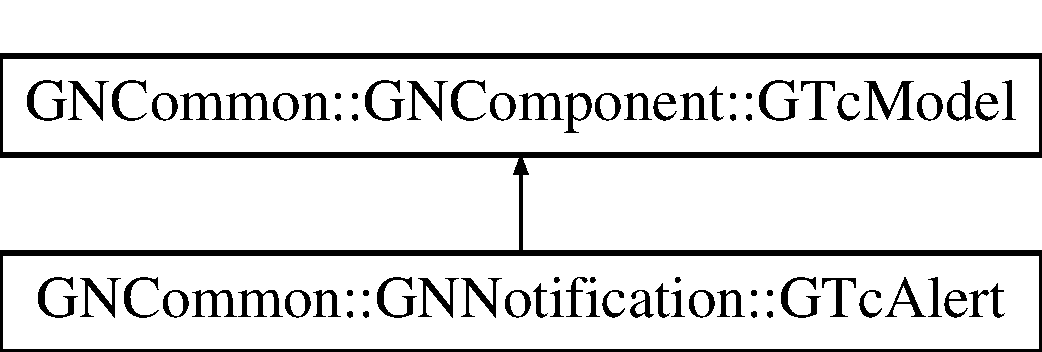
\includegraphics[height=2.000000cm]{class_g_n_common_1_1_g_n_component_1_1_g_tc_model}
\end{center}
\end{figure}
\subsection*{Public Attributes}
\begin{DoxyCompactItemize}
\item 
\mbox{\Hypertarget{class_g_n_common_1_1_g_n_component_1_1_g_tc_model_a4d953e4b7f0b66c7eabd8ce6c91d120b}\label{class_g_n_common_1_1_g_n_component_1_1_g_tc_model_a4d953e4b7f0b66c7eabd8ce6c91d120b}} 
\mbox{\hyperlink{class_g_n_common_1_1_g_n_component_1_1_g_tc_event}{G\+Tc\+Event}}$<$ xui\+Max\+Listeners $>$ {\bfseries Vo\+Event}
\end{DoxyCompactItemize}
\subsection*{Static Protected Attributes}
\begin{DoxyCompactItemize}
\item 
\mbox{\Hypertarget{class_g_n_common_1_1_g_n_component_1_1_g_tc_model_ac1558cfb8f84addcdf0a2fa6457ee760}\label{class_g_n_common_1_1_g_n_component_1_1_g_tc_model_ac1558cfb8f84addcdf0a2fa6457ee760}} 
static const \mbox{\hyperlink{namespace_g_n_common_a941b527ef318f318aed7903dc832b7e4}{Tu32}} {\bfseries xui\+Max\+Listeners} = 16
\end{DoxyCompactItemize}


\subsection{Detailed Description}


Definition at line \mbox{\hyperlink{_model_8h_source_l00007}{7}} of file \mbox{\hyperlink{_model_8h_source}{Model.\+h}}.



The documentation for this class was generated from the following files\+:\begin{DoxyCompactItemize}
\item 
C\+:/\+Projects/\+Bergermeister\+Home/\+Software/\+Common/inc/\+Component/Model.\+h\item 
C\+:/\+Projects/\+Bergermeister\+Home/\+Software/\+Common/src/\+Component/Model.\+cpp\end{DoxyCompactItemize}

\hypertarget{class_g_n_common_1_1_g_n_serial_1_1_g_tc_port}{}\section{G\+N\+Common\+:\+:G\+N\+Serial\+:\+:G\+Tc\+Port Class Reference}
\label{class_g_n_common_1_1_g_n_serial_1_1_g_tc_port}\index{G\+N\+Common\+::\+G\+N\+Serial\+::\+G\+Tc\+Port@{G\+N\+Common\+::\+G\+N\+Serial\+::\+G\+Tc\+Port}}
\subsection*{Public Member Functions}
\begin{DoxyCompactItemize}
\item 
\mbox{\Hypertarget{class_g_n_common_1_1_g_n_serial_1_1_g_tc_port_af8f4ea81da23337f7f0b5ba492d6c310}\label{class_g_n_common_1_1_g_n_serial_1_1_g_tc_port_af8f4ea81da23337f7f0b5ba492d6c310}} 
\mbox{\hyperlink{namespace_g_n_common_a6b5283329f609e2175dd0c91fc1520ba}{G\+Tb8}} {\bfseries M\+Open} (void)
\end{DoxyCompactItemize}


\subsection{Detailed Description}


Definition at line 14 of file Port.\+h.



The documentation for this class was generated from the following files\+:\begin{DoxyCompactItemize}
\item 
C\+:/\+Projects/\+Bergermeister\+Home/\+Serial/Port.\+h\item 
C\+:/\+Projects/\+Bergermeister\+Home/\+Serial/Port.\+cpp\end{DoxyCompactItemize}

\hypertarget{class_g_n_common_1_1_g_n_containers_1_1_g_tc_queue}{}\section{G\+N\+Common\+:\+:G\+N\+Containers\+:\+:G\+Tc\+Queue$<$ G\+Tc\+Type $>$ Class Template Reference}
\label{class_g_n_common_1_1_g_n_containers_1_1_g_tc_queue}\index{G\+N\+Common\+::\+G\+N\+Containers\+::\+G\+Tc\+Queue$<$ G\+Tc\+Type $>$@{G\+N\+Common\+::\+G\+N\+Containers\+::\+G\+Tc\+Queue$<$ G\+Tc\+Type $>$}}
\subsection*{Public Member Functions}
\begin{DoxyCompactItemize}
\item 
\mbox{\Hypertarget{class_g_n_common_1_1_g_n_containers_1_1_g_tc_queue_af221d0c44b40c12e79ff489a2098f99b}\label{class_g_n_common_1_1_g_n_containers_1_1_g_tc_queue_af221d0c44b40c12e79ff489a2098f99b}} 
{\bfseries G\+Tc\+Queue} (G\+Tc\+Type $\ast$aop\+Buffer, \mbox{\hyperlink{namespace_g_n_common_a941b527ef318f318aed7903dc832b7e4}{Tu32}} aui\+Size)
\item 
\mbox{\Hypertarget{class_g_n_common_1_1_g_n_containers_1_1_g_tc_queue_adcd51c7ec007494bc5dfb5a942a0b3e2}\label{class_g_n_common_1_1_g_n_containers_1_1_g_tc_queue_adcd51c7ec007494bc5dfb5a942a0b3e2}} 
\mbox{\hyperlink{namespace_g_n_common_a8115dc7ed53b6e5b52e6bfde1632ea74}{Tb8}} {\bfseries M\+Enqueue} (G\+Tc\+Type \&aor\+Element)
\item 
\mbox{\Hypertarget{class_g_n_common_1_1_g_n_containers_1_1_g_tc_queue_ad2e1a8dc45f1759c735459b2be6ffc6d}\label{class_g_n_common_1_1_g_n_containers_1_1_g_tc_queue_ad2e1a8dc45f1759c735459b2be6ffc6d}} 
\mbox{\hyperlink{namespace_g_n_common_a8115dc7ed53b6e5b52e6bfde1632ea74}{Tb8}} {\bfseries M\+Dequeue} (G\+Tc\+Type \&aor\+Element)
\item 
\mbox{\Hypertarget{class_g_n_common_1_1_g_n_containers_1_1_g_tc_queue_a8e915719d76a75aacca2366c77218472}\label{class_g_n_common_1_1_g_n_containers_1_1_g_tc_queue_a8e915719d76a75aacca2366c77218472}} 
\mbox{\hyperlink{namespace_g_n_common_a8115dc7ed53b6e5b52e6bfde1632ea74}{Tb8}} {\bfseries M\+Is\+Empty} (void) const
\item 
\mbox{\Hypertarget{class_g_n_common_1_1_g_n_containers_1_1_g_tc_queue_a3cddbe06ba953e4de67ae00c3fb20b77}\label{class_g_n_common_1_1_g_n_containers_1_1_g_tc_queue_a3cddbe06ba953e4de67ae00c3fb20b77}} 
\mbox{\hyperlink{namespace_g_n_common_a8115dc7ed53b6e5b52e6bfde1632ea74}{Tb8}} {\bfseries M\+Is\+Full} (void) const
\item 
\mbox{\Hypertarget{class_g_n_common_1_1_g_n_containers_1_1_g_tc_queue_aa0328d6bf5a6c9d32a8be8bbe00e2950}\label{class_g_n_common_1_1_g_n_containers_1_1_g_tc_queue_aa0328d6bf5a6c9d32a8be8bbe00e2950}} 
\mbox{\hyperlink{namespace_g_n_common_a941b527ef318f318aed7903dc832b7e4}{Tu32}} {\bfseries M\+Count} (void) const
\end{DoxyCompactItemize}


\subsection{Detailed Description}
\subsubsection*{template$<$class G\+Tc\+Type$>$\newline
class G\+N\+Common\+::\+G\+N\+Containers\+::\+G\+Tc\+Queue$<$ G\+Tc\+Type $>$}



Definition at line \mbox{\hyperlink{_queue_8h_source_l00008}{8}} of file \mbox{\hyperlink{_queue_8h_source}{Queue.\+h}}.



The documentation for this class was generated from the following file\+:\begin{DoxyCompactItemize}
\item 
C\+:/\+Projects/\+Bergermeister\+Home/\+Software/\+Common/inc/\+Containers/Queue.\+h\end{DoxyCompactItemize}

\hypertarget{class_g_n_common_1_1_g_tc_stop_watch}{}\section{G\+N\+Common\+:\+:G\+Tc\+Stop\+Watch Class Reference}
\label{class_g_n_common_1_1_g_tc_stop_watch}\index{G\+N\+Common\+::\+G\+Tc\+Stop\+Watch@{G\+N\+Common\+::\+G\+Tc\+Stop\+Watch}}
\subsection*{Public Member Functions}
\begin{DoxyCompactItemize}
\item 
\mbox{\Hypertarget{class_g_n_common_1_1_g_tc_stop_watch_ae442c6e313df8f2ad22b4ceef71b89ab}\label{class_g_n_common_1_1_g_tc_stop_watch_ae442c6e313df8f2ad22b4ceef71b89ab}} 
{\bfseries G\+Tc\+Stop\+Watch} (const \mbox{\hyperlink{class_g_n_common_1_1_g_tc_stop_watch}{G\+Tc\+Stop\+Watch}} \&aor\+Stop\+Watch)
\item 
\mbox{\Hypertarget{class_g_n_common_1_1_g_tc_stop_watch_a334776e4f98289f2093b2da4cf3cb8b8}\label{class_g_n_common_1_1_g_tc_stop_watch_a334776e4f98289f2093b2da4cf3cb8b8}} 
\mbox{\hyperlink{class_g_n_common_1_1_g_tc_stop_watch}{G\+Tc\+Stop\+Watch}} \& {\bfseries operator=} (const \mbox{\hyperlink{class_g_n_common_1_1_g_tc_stop_watch}{G\+Tc\+Stop\+Watch}} \&aor\+Stop\+Watch)
\item 
\mbox{\Hypertarget{class_g_n_common_1_1_g_tc_stop_watch_ad62dfcb669827907489089ff31be6325}\label{class_g_n_common_1_1_g_tc_stop_watch_ad62dfcb669827907489089ff31be6325}} 
void {\bfseries M\+Start} (void)
\item 
\mbox{\Hypertarget{class_g_n_common_1_1_g_tc_stop_watch_ac9d0bf8c49268056b6b4d9486fdaade6}\label{class_g_n_common_1_1_g_tc_stop_watch_ac9d0bf8c49268056b6b4d9486fdaade6}} 
\mbox{\hyperlink{namespace_g_n_common_a01e8527dabf7ab4f123156b0701945eb}{G\+Tu64}} {\bfseries M\+Stop} (void)
\item 
\mbox{\Hypertarget{class_g_n_common_1_1_g_tc_stop_watch_a2fdbb8f6ed275c1601c2b52a530fd045}\label{class_g_n_common_1_1_g_tc_stop_watch_a2fdbb8f6ed275c1601c2b52a530fd045}} 
\mbox{\hyperlink{namespace_g_n_common_a01e8527dabf7ab4f123156b0701945eb}{G\+Tu64}} {\bfseries M\+Elapsed} (void)
\end{DoxyCompactItemize}
\subsection*{Protected Attributes}
\begin{DoxyCompactItemize}
\item 
\mbox{\Hypertarget{class_g_n_common_1_1_g_tc_stop_watch_a48e00f31a5f0d2ec9bf4678e3ea8bc0a}\label{class_g_n_common_1_1_g_tc_stop_watch_a48e00f31a5f0d2ec9bf4678e3ea8bc0a}} 
L\+A\+R\+G\+E\+\_\+\+I\+N\+T\+E\+G\+ER {\bfseries vo\+Start}
\item 
\mbox{\Hypertarget{class_g_n_common_1_1_g_tc_stop_watch_a0c7c046a1a57282bf389af72252410f6}\label{class_g_n_common_1_1_g_tc_stop_watch_a0c7c046a1a57282bf389af72252410f6}} 
L\+A\+R\+G\+E\+\_\+\+I\+N\+T\+E\+G\+ER {\bfseries vo\+End}
\item 
\mbox{\Hypertarget{class_g_n_common_1_1_g_tc_stop_watch_a8b50e42107f8f88743eea8856fe85dd5}\label{class_g_n_common_1_1_g_tc_stop_watch_a8b50e42107f8f88743eea8856fe85dd5}} 
\mbox{\hyperlink{namespace_g_n_common_a6b5283329f609e2175dd0c91fc1520ba}{G\+Tb8}} {\bfseries vb\+Running}
\end{DoxyCompactItemize}
\subsection*{Static Protected Attributes}
\begin{DoxyCompactItemize}
\item 
\mbox{\Hypertarget{class_g_n_common_1_1_g_tc_stop_watch_ae1b92efd901fed6c6de030fc9112a15f}\label{class_g_n_common_1_1_g_tc_stop_watch_ae1b92efd901fed6c6de030fc9112a15f}} 
static const L\+O\+N\+G\+L\+O\+NG {\bfseries xl\+Max\+Quad\+Part} = 9223372036854775807
\item 
\mbox{\Hypertarget{class_g_n_common_1_1_g_tc_stop_watch_ac9ff802e3258165d18f566ffe6bd6fc1}\label{class_g_n_common_1_1_g_tc_stop_watch_ac9ff802e3258165d18f566ffe6bd6fc1}} 
static const \mbox{\hyperlink{namespace_g_n_common_a01e8527dabf7ab4f123156b0701945eb}{G\+Tu64}} {\bfseries xul\+Time\+Base} = 1000000\+LL
\item 
\mbox{\Hypertarget{class_g_n_common_1_1_g_tc_stop_watch_afd7212375fb1201a16f966430dfcc30d}\label{class_g_n_common_1_1_g_tc_stop_watch_afd7212375fb1201a16f966430dfcc30d}} 
static \mbox{\hyperlink{namespace_g_n_common_a01e8527dabf7ab4f123156b0701945eb}{G\+Tu64}} {\bfseries vul\+Frequency} = 0
\end{DoxyCompactItemize}


\subsection{Detailed Description}


Definition at line 5 of file Stop\+Watch.\+h.



The documentation for this class was generated from the following files\+:\begin{DoxyCompactItemize}
\item 
C\+:/\+Projects/\+Bergermeister\+Home/\+Common/\+Source/Stop\+Watch.\+h\item 
C\+:/\+Projects/\+Bergermeister\+Home/\+Common/\+Source/Stop\+Watch.\+cpp\end{DoxyCompactItemize}

\hypertarget{struct_identifier}{}\section{Identifier Struct Reference}
\label{struct_identifier}\index{Identifier@{Identifier}}


The documentation for this struct was generated from the following file\+:\begin{DoxyCompactItemize}
\item 
C\+:/\+Projects/\+Bergermeister\+Home/\+Common/\+Source/\mbox{\hyperlink{_alert_8h}{Alert.\+h}}\end{DoxyCompactItemize}

\hypertarget{class_xaml_binding_info_1_1_i_xaml_bindings}{}\section{Xaml\+Binding\+Info\+:\+:I\+Xaml\+Bindings Class Reference}
\label{class_xaml_binding_info_1_1_i_xaml_bindings}\index{Xaml\+Binding\+Info\+::\+I\+Xaml\+Bindings@{Xaml\+Binding\+Info\+::\+I\+Xaml\+Bindings}}
\subsection*{Public Member Functions}
\begin{DoxyCompactItemize}
\item 
\mbox{\Hypertarget{class_xaml_binding_info_1_1_i_xaml_bindings_a84ac9cebecf96c2c7ccfaeb43e9d4252}\label{class_xaml_binding_info_1_1_i_xaml_bindings_a84ac9cebecf96c2c7ccfaeb43e9d4252}} 
virtual bool {\bfseries Is\+Initialized} ()=0
\item 
\mbox{\Hypertarget{class_xaml_binding_info_1_1_i_xaml_bindings_af7bbb67de71bfaedbf116df6d689f22b}\label{class_xaml_binding_info_1_1_i_xaml_bindings_af7bbb67de71bfaedbf116df6d689f22b}} 
virtual void {\bfseries Update} ()=0
\item 
\mbox{\Hypertarget{class_xaml_binding_info_1_1_i_xaml_bindings_a35a0a9b1922e3c719c26791bdc0a102e}\label{class_xaml_binding_info_1_1_i_xaml_bindings_a35a0a9b1922e3c719c26791bdc0a102e}} 
virtual bool {\bfseries Set\+Data\+Root} (\+::Platform\+::\+Object$^\wedge$ data)=0
\item 
\mbox{\Hypertarget{class_xaml_binding_info_1_1_i_xaml_bindings_abbffa5e36a4cc1ef3b7e14814112480a}\label{class_xaml_binding_info_1_1_i_xaml_bindings_abbffa5e36a4cc1ef3b7e14814112480a}} 
virtual void {\bfseries Stop\+Tracking} ()=0
\item 
\mbox{\Hypertarget{class_xaml_binding_info_1_1_i_xaml_bindings_a9e14f106ac9c9a8fef1203dc34619865}\label{class_xaml_binding_info_1_1_i_xaml_bindings_a9e14f106ac9c9a8fef1203dc34619865}} 
virtual void {\bfseries Connect} (int connection\+Id, \+::Platform\+::\+Object$^\wedge$ target)=0
\item 
\mbox{\Hypertarget{class_xaml_binding_info_1_1_i_xaml_bindings_a38efcb61569708b5807d32478b66b6be}\label{class_xaml_binding_info_1_1_i_xaml_bindings_a38efcb61569708b5807d32478b66b6be}} 
virtual void {\bfseries Reset\+Template} ()=0
\item 
\mbox{\Hypertarget{class_xaml_binding_info_1_1_i_xaml_bindings_a9a6d53b4fae9f58a529b914e60f6a6b1}\label{class_xaml_binding_info_1_1_i_xaml_bindings_a9a6d53b4fae9f58a529b914e60f6a6b1}} 
virtual int {\bfseries Process\+Bindings} (\+::Windows\+::\+U\+I\+::\+Xaml\+::\+Controls\+::\+Container\+Content\+Changing\+Event\+Args$^\wedge$ args)=0
\item 
\mbox{\Hypertarget{class_xaml_binding_info_1_1_i_xaml_bindings_a9a6e60fee37d0cf53ccebc9d8c07d90f}\label{class_xaml_binding_info_1_1_i_xaml_bindings_a9a6e60fee37d0cf53ccebc9d8c07d90f}} 
virtual void {\bfseries Subscribe\+For\+Data\+Context\+Changed} (\+::Windows\+::\+U\+I\+::\+Xaml\+::\+Framework\+Element$^\wedge$ object, \+::\mbox{\hyperlink{class_xaml_binding_info_1_1_xaml_bindings}{Xaml\+Binding\+Info\+::\+Xaml\+Bindings}}$^\wedge$ handler)=0
\item 
\mbox{\Hypertarget{class_xaml_binding_info_1_1_i_xaml_bindings_a84ac9cebecf96c2c7ccfaeb43e9d4252}\label{class_xaml_binding_info_1_1_i_xaml_bindings_a84ac9cebecf96c2c7ccfaeb43e9d4252}} 
virtual bool {\bfseries Is\+Initialized} ()=0
\item 
\mbox{\Hypertarget{class_xaml_binding_info_1_1_i_xaml_bindings_af7bbb67de71bfaedbf116df6d689f22b}\label{class_xaml_binding_info_1_1_i_xaml_bindings_af7bbb67de71bfaedbf116df6d689f22b}} 
virtual void {\bfseries Update} ()=0
\item 
\mbox{\Hypertarget{class_xaml_binding_info_1_1_i_xaml_bindings_a35a0a9b1922e3c719c26791bdc0a102e}\label{class_xaml_binding_info_1_1_i_xaml_bindings_a35a0a9b1922e3c719c26791bdc0a102e}} 
virtual bool {\bfseries Set\+Data\+Root} (\+::Platform\+::\+Object$^\wedge$ data)=0
\item 
\mbox{\Hypertarget{class_xaml_binding_info_1_1_i_xaml_bindings_abbffa5e36a4cc1ef3b7e14814112480a}\label{class_xaml_binding_info_1_1_i_xaml_bindings_abbffa5e36a4cc1ef3b7e14814112480a}} 
virtual void {\bfseries Stop\+Tracking} ()=0
\item 
\mbox{\Hypertarget{class_xaml_binding_info_1_1_i_xaml_bindings_a9e14f106ac9c9a8fef1203dc34619865}\label{class_xaml_binding_info_1_1_i_xaml_bindings_a9e14f106ac9c9a8fef1203dc34619865}} 
virtual void {\bfseries Connect} (int connection\+Id, \+::Platform\+::\+Object$^\wedge$ target)=0
\item 
\mbox{\Hypertarget{class_xaml_binding_info_1_1_i_xaml_bindings_a38efcb61569708b5807d32478b66b6be}\label{class_xaml_binding_info_1_1_i_xaml_bindings_a38efcb61569708b5807d32478b66b6be}} 
virtual void {\bfseries Reset\+Template} ()=0
\item 
\mbox{\Hypertarget{class_xaml_binding_info_1_1_i_xaml_bindings_a9a6d53b4fae9f58a529b914e60f6a6b1}\label{class_xaml_binding_info_1_1_i_xaml_bindings_a9a6d53b4fae9f58a529b914e60f6a6b1}} 
virtual int {\bfseries Process\+Bindings} (\+::Windows\+::\+U\+I\+::\+Xaml\+::\+Controls\+::\+Container\+Content\+Changing\+Event\+Args$^\wedge$ args)=0
\item 
\mbox{\Hypertarget{class_xaml_binding_info_1_1_i_xaml_bindings_a9a6e60fee37d0cf53ccebc9d8c07d90f}\label{class_xaml_binding_info_1_1_i_xaml_bindings_a9a6e60fee37d0cf53ccebc9d8c07d90f}} 
virtual void {\bfseries Subscribe\+For\+Data\+Context\+Changed} (\+::Windows\+::\+U\+I\+::\+Xaml\+::\+Framework\+Element$^\wedge$ object, \+::\mbox{\hyperlink{class_xaml_binding_info_1_1_xaml_bindings}{Xaml\+Binding\+Info\+::\+Xaml\+Bindings}}$^\wedge$ handler)=0
\end{DoxyCompactItemize}


\subsection{Detailed Description}


Definition at line 15 of file Xaml\+Binding\+Info.\+g.\+h.



The documentation for this class was generated from the following file\+:\begin{DoxyCompactItemize}
\item 
C\+:/\+Projects/\+Bergermeister\+Home/\+Console/\+Generated Files/Xaml\+Binding\+Info.\+g.\+h\end{DoxyCompactItemize}

\hypertarget{class_console_1_1_main_page}{}\section{Console\+:\+:Main\+Page Class Reference}
\label{class_console_1_1_main_page}\index{Console\+::\+Main\+Page@{Console\+::\+Main\+Page}}


An empty page that can be used on its own or navigated to within a Frame.  




{\ttfamily \#include $<$Main\+Page.\+xaml.\+h$>$}



Inheritance diagram for Console\+:\+:Main\+Page\+:\nopagebreak
\begin{figure}[H]
\begin{center}
\leavevmode
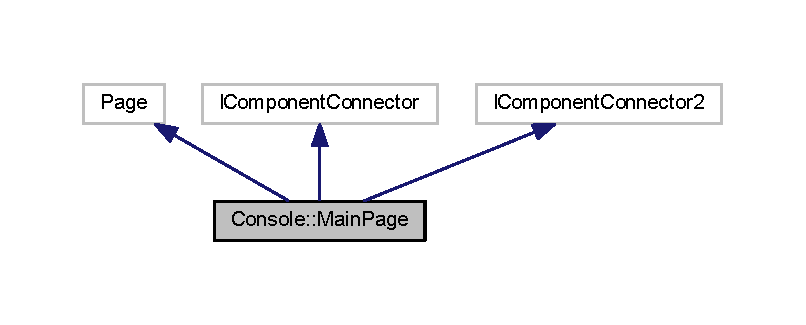
\includegraphics[width=350pt]{class_console_1_1_main_page__inherit__graph}
\end{center}
\end{figure}


Collaboration diagram for Console\+:\+:Main\+Page\+:\nopagebreak
\begin{figure}[H]
\begin{center}
\leavevmode
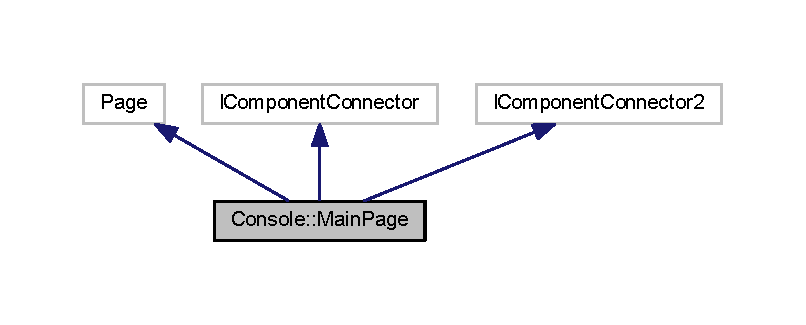
\includegraphics[width=350pt]{class_console_1_1_main_page__coll__graph}
\end{center}
\end{figure}
\subsection*{Public Member Functions}
\begin{DoxyCompactItemize}
\item 
\mbox{\Hypertarget{class_console_1_1_main_page_a6bb795510044a28234a66b9a6c957c52}\label{class_console_1_1_main_page_a6bb795510044a28234a66b9a6c957c52}} 
void {\bfseries Initialize\+Component} ()
\item 
\mbox{\Hypertarget{class_console_1_1_main_page_a6f1a1833bf7cd5055b249114d066cc5f}\label{class_console_1_1_main_page_a6f1a1833bf7cd5055b249114d066cc5f}} 
virtual void {\bfseries Connect} (int connection\+Id, \+::Platform\+::\+Object$^\wedge$ target)
\item 
\mbox{\Hypertarget{class_console_1_1_main_page_af11786f4a1d1244e44ca0c505873d32a}\label{class_console_1_1_main_page_af11786f4a1d1244e44ca0c505873d32a}} 
virtual \+::Windows\+::\+U\+I\+::\+Xaml\+::\+Markup\+::\+I\+Component\+Connector $^\wedge$ {\bfseries Get\+Binding\+Connector} (int connection\+Id, \+::Platform\+::\+Object$^\wedge$ target)
\end{DoxyCompactItemize}


\subsection{Detailed Description}
An empty page that can be used on its own or navigated to within a Frame. 



Definition at line 23 of file Main\+Page.\+g.\+h.



The documentation for this class was generated from the following files\+:\begin{DoxyCompactItemize}
\item 
C\+:/\+Projects/\+Bergermeister\+Home/\+Console/\+Generated Files/Main\+Page.\+g.\+h\item 
C\+:/\+Projects/\+Bergermeister\+Home/\+Console/Main\+Page.\+xaml.\+h\item 
C\+:/\+Projects/\+Bergermeister\+Home/\+Console/Main\+Page.\+xaml.\+cpp\end{DoxyCompactItemize}

\hypertarget{class_thermostat_1_1_main_page}{}\section{Thermostat\+:\+:Main\+Page Class Reference}
\label{class_thermostat_1_1_main_page}\index{Thermostat\+::\+Main\+Page@{Thermostat\+::\+Main\+Page}}


An empty page that can be used on its own or navigated to within a Frame.  




{\ttfamily \#include $<$Main\+Page.\+xaml.\+h$>$}



Inheritance diagram for Thermostat\+:\+:Main\+Page\+:\nopagebreak
\begin{figure}[H]
\begin{center}
\leavevmode
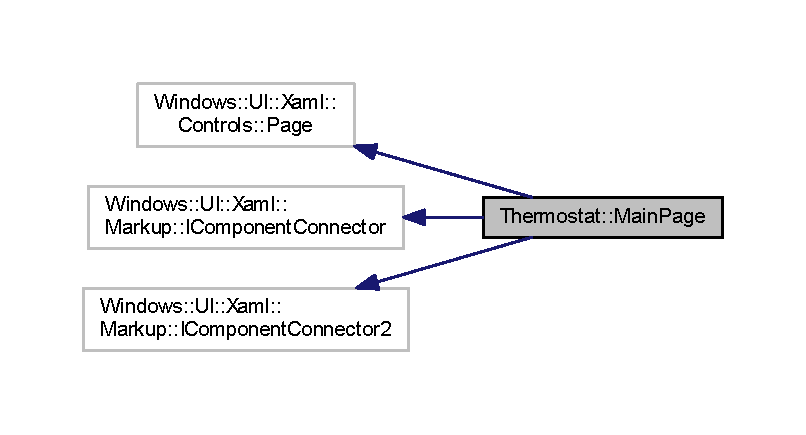
\includegraphics[width=350pt]{class_thermostat_1_1_main_page__inherit__graph}
\end{center}
\end{figure}


Collaboration diagram for Thermostat\+:\+:Main\+Page\+:\nopagebreak
\begin{figure}[H]
\begin{center}
\leavevmode
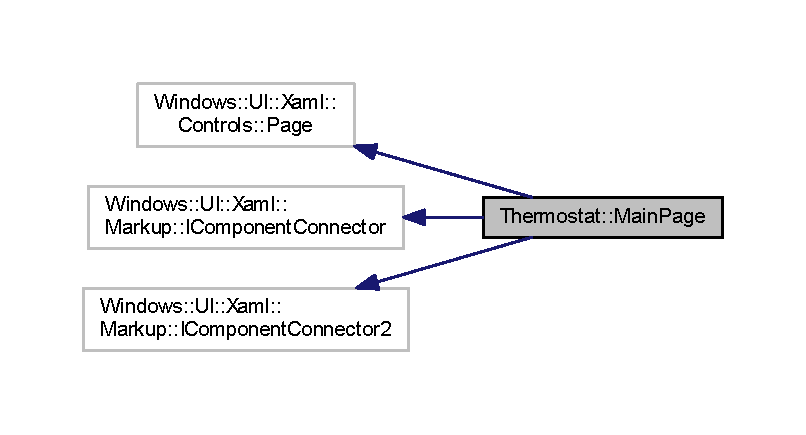
\includegraphics[width=350pt]{class_thermostat_1_1_main_page__coll__graph}
\end{center}
\end{figure}
\subsection*{Public Member Functions}
\begin{DoxyCompactItemize}
\item 
\mbox{\Hypertarget{class_thermostat_1_1_main_page_ae9613bb5ad8c05464cb4786b9707f820}\label{class_thermostat_1_1_main_page_ae9613bb5ad8c05464cb4786b9707f820}} 
void {\bfseries Initialize\+Component} ()
\item 
\mbox{\Hypertarget{class_thermostat_1_1_main_page_a2f3855785b4919891ed16dc79f1a7ba8}\label{class_thermostat_1_1_main_page_a2f3855785b4919891ed16dc79f1a7ba8}} 
virtual void {\bfseries Connect} (int connection\+Id, \+::Platform\+::\+Object$^\wedge$ target)
\item 
\mbox{\Hypertarget{class_thermostat_1_1_main_page_ab3268e3a8be780fc55e3ed2856f2e6d4}\label{class_thermostat_1_1_main_page_ab3268e3a8be780fc55e3ed2856f2e6d4}} 
virtual \+::Windows\+::\+U\+I\+::\+Xaml\+::\+Markup\+::\+I\+Component\+Connector $^\wedge$ {\bfseries Get\+Binding\+Connector} (int connection\+Id, \+::Platform\+::\+Object$^\wedge$ target)
\end{DoxyCompactItemize}
\subsection*{Protected Member Functions}
\begin{DoxyCompactItemize}
\item 
\mbox{\Hypertarget{class_thermostat_1_1_main_page_ab3aa395384bce595509a9926d4d89cab}\label{class_thermostat_1_1_main_page_ab3aa395384bce595509a9926d4d89cab}} 
void {\bfseries Page\+\_\+\+Loaded} (Platform\+::\+Object$^\wedge$ aop\+Sender, Windows\+::\+U\+I\+::\+Xaml\+::\+Routed\+Event\+Args$^\wedge$ aop\+Args)
\item 
\mbox{\Hypertarget{class_thermostat_1_1_main_page_a790bf7e5e64ba6af4bb5fd2e1d527f64}\label{class_thermostat_1_1_main_page_a790bf7e5e64ba6af4bb5fd2e1d527f64}} 
void {\bfseries M\+Timer\+Elapsed} (Windows\+::\+System\+::\+Threading\+::\+Thread\+Pool\+Timer$^\wedge$ aop\+Timer)
\end{DoxyCompactItemize}


\subsection{Detailed Description}
An empty page that can be used on its own or navigated to within a Frame. 



Definition at line 23 of file Main\+Page.\+g.\+h.



The documentation for this class was generated from the following files\+:\begin{DoxyCompactItemize}
\item 
C\+:/\+Projects/\+Bergermeister\+Home/\+Thermostat/\+Generated Files/Main\+Page.\+g.\+h\item 
C\+:/\+Projects/\+Bergermeister\+Home/\+Thermostat/Main\+Page.\+xaml.\+h\item 
C\+:/\+Projects/\+Bergermeister\+Home/\+Thermostat/\+Generated Files/Main\+Page.\+g.\+hpp\item 
C\+:/\+Projects/\+Bergermeister\+Home/\+Thermostat/Main\+Page.\+xaml.\+cpp\end{DoxyCompactItemize}

\hypertarget{struct_status}{}\section{Status Struct Reference}
\label{struct_status}\index{Status@{Status}}


The documentation for this struct was generated from the following file\+:\begin{DoxyCompactItemize}
\item 
C\+:/\+Projects/\+Bergermeister\+Home/\+Common/\+Source/\mbox{\hyperlink{_alert_8h}{Alert.\+h}}\end{DoxyCompactItemize}

\hypertarget{struct_g_n_common_1_1_g_tc_alert_1_1_ts_identifier}{}\section{G\+N\+Common\+:\+:G\+Tc\+Alert\+:\+:Ts\+Identifier Struct Reference}
\label{struct_g_n_common_1_1_g_tc_alert_1_1_ts_identifier}\index{G\+N\+Common\+::\+G\+Tc\+Alert\+::\+Ts\+Identifier@{G\+N\+Common\+::\+G\+Tc\+Alert\+::\+Ts\+Identifier}}
\subsection*{Public Attributes}
\begin{DoxyCompactItemize}
\item 
\mbox{\hyperlink{namespace_g_n_common_ae5485474bc8f23e462e920a17b377b53}{G\+Tu32}} \mbox{\hyperlink{struct_g_n_common_1_1_g_tc_alert_1_1_ts_identifier_a83bb4d784e9f8d772b79a2faab4c279c}{vui\+Index}}\+: 8
\item 
\mbox{\hyperlink{class_g_n_common_1_1_g_tc_alert_a2deb7f82fcf5d88b4e10d74fa6c28cb7}{Te\+Group}} \mbox{\hyperlink{struct_g_n_common_1_1_g_tc_alert_1_1_ts_identifier_af23bb4b61df8abb45a4a77162a91e980}{ve\+Group}}\+: 8
\item 
\mbox{\hyperlink{class_g_n_common_1_1_g_tc_alert_aec0a7908321c01ae225df4908d7f3fa0}{Te\+Component}} \mbox{\hyperlink{struct_g_n_common_1_1_g_tc_alert_1_1_ts_identifier_ac500c0db17c543fec720ef745966a53b}{ve\+Comp\+Det}}\+: 8
\item 
\mbox{\hyperlink{class_g_n_common_1_1_g_tc_alert_aec0a7908321c01ae225df4908d7f3fa0}{Te\+Component}} \mbox{\hyperlink{struct_g_n_common_1_1_g_tc_alert_1_1_ts_identifier_a410931b980bb13ee9eeece7f69c576b1}{ve\+Comp\+Gen}}\+: 8
\end{DoxyCompactItemize}


\subsection{Detailed Description}


Definition at line 52 of file Alert.\+h.



\subsection{Member Data Documentation}
\mbox{\Hypertarget{struct_g_n_common_1_1_g_tc_alert_1_1_ts_identifier_ac500c0db17c543fec720ef745966a53b}\label{struct_g_n_common_1_1_g_tc_alert_1_1_ts_identifier_ac500c0db17c543fec720ef745966a53b}} 
\index{G\+N\+Common\+::\+G\+Tc\+Alert\+::\+Ts\+Identifier@{G\+N\+Common\+::\+G\+Tc\+Alert\+::\+Ts\+Identifier}!ve\+Comp\+Det@{ve\+Comp\+Det}}
\index{ve\+Comp\+Det@{ve\+Comp\+Det}!G\+N\+Common\+::\+G\+Tc\+Alert\+::\+Ts\+Identifier@{G\+N\+Common\+::\+G\+Tc\+Alert\+::\+Ts\+Identifier}}
\subsubsection{\texorpdfstring{ve\+Comp\+Det}{veCompDet}}
{\footnotesize\ttfamily \mbox{\hyperlink{class_g_n_common_1_1_g_tc_alert_aec0a7908321c01ae225df4908d7f3fa0}{Te\+Component}} G\+N\+Common\+::\+G\+Tc\+Alert\+::\+Ts\+Identifier\+::ve\+Comp\+Det}

Bits 16 -\/ 23 \+: Detecting Component 

Definition at line 56 of file Alert.\+h.

\mbox{\Hypertarget{struct_g_n_common_1_1_g_tc_alert_1_1_ts_identifier_a410931b980bb13ee9eeece7f69c576b1}\label{struct_g_n_common_1_1_g_tc_alert_1_1_ts_identifier_a410931b980bb13ee9eeece7f69c576b1}} 
\index{G\+N\+Common\+::\+G\+Tc\+Alert\+::\+Ts\+Identifier@{G\+N\+Common\+::\+G\+Tc\+Alert\+::\+Ts\+Identifier}!ve\+Comp\+Gen@{ve\+Comp\+Gen}}
\index{ve\+Comp\+Gen@{ve\+Comp\+Gen}!G\+N\+Common\+::\+G\+Tc\+Alert\+::\+Ts\+Identifier@{G\+N\+Common\+::\+G\+Tc\+Alert\+::\+Ts\+Identifier}}
\subsubsection{\texorpdfstring{ve\+Comp\+Gen}{veCompGen}}
{\footnotesize\ttfamily \mbox{\hyperlink{class_g_n_common_1_1_g_tc_alert_aec0a7908321c01ae225df4908d7f3fa0}{Te\+Component}} G\+N\+Common\+::\+G\+Tc\+Alert\+::\+Ts\+Identifier\+::ve\+Comp\+Gen}

Bits 24 -\/ 31 \+: Generating Component 

Definition at line 57 of file Alert.\+h.

\mbox{\Hypertarget{struct_g_n_common_1_1_g_tc_alert_1_1_ts_identifier_af23bb4b61df8abb45a4a77162a91e980}\label{struct_g_n_common_1_1_g_tc_alert_1_1_ts_identifier_af23bb4b61df8abb45a4a77162a91e980}} 
\index{G\+N\+Common\+::\+G\+Tc\+Alert\+::\+Ts\+Identifier@{G\+N\+Common\+::\+G\+Tc\+Alert\+::\+Ts\+Identifier}!ve\+Group@{ve\+Group}}
\index{ve\+Group@{ve\+Group}!G\+N\+Common\+::\+G\+Tc\+Alert\+::\+Ts\+Identifier@{G\+N\+Common\+::\+G\+Tc\+Alert\+::\+Ts\+Identifier}}
\subsubsection{\texorpdfstring{ve\+Group}{veGroup}}
{\footnotesize\ttfamily \mbox{\hyperlink{class_g_n_common_1_1_g_tc_alert_a2deb7f82fcf5d88b4e10d74fa6c28cb7}{Te\+Group}} G\+N\+Common\+::\+G\+Tc\+Alert\+::\+Ts\+Identifier\+::ve\+Group}

Bits 8 -\/ 15 \+: Group 

Definition at line 55 of file Alert.\+h.

\mbox{\Hypertarget{struct_g_n_common_1_1_g_tc_alert_1_1_ts_identifier_a83bb4d784e9f8d772b79a2faab4c279c}\label{struct_g_n_common_1_1_g_tc_alert_1_1_ts_identifier_a83bb4d784e9f8d772b79a2faab4c279c}} 
\index{G\+N\+Common\+::\+G\+Tc\+Alert\+::\+Ts\+Identifier@{G\+N\+Common\+::\+G\+Tc\+Alert\+::\+Ts\+Identifier}!vui\+Index@{vui\+Index}}
\index{vui\+Index@{vui\+Index}!G\+N\+Common\+::\+G\+Tc\+Alert\+::\+Ts\+Identifier@{G\+N\+Common\+::\+G\+Tc\+Alert\+::\+Ts\+Identifier}}
\subsubsection{\texorpdfstring{vui\+Index}{vuiIndex}}
{\footnotesize\ttfamily \mbox{\hyperlink{namespace_g_n_common_ae5485474bc8f23e462e920a17b377b53}{G\+Tu32}} G\+N\+Common\+::\+G\+Tc\+Alert\+::\+Ts\+Identifier\+::vui\+Index}

Bits 0 -\/ 7 \+: Index 

Definition at line 54 of file Alert.\+h.



The documentation for this struct was generated from the following file\+:\begin{DoxyCompactItemize}
\item 
C\+:/\+Projects/\+Bergermeister\+Home/\+Common/\+Source/\mbox{\hyperlink{_alert_8h}{Alert.\+h}}\end{DoxyCompactItemize}

\hypertarget{struct_g_n_common_1_1_g_tc_alert_1_1_ts_status}{}\section{G\+N\+Common\+:\+:G\+Tc\+Alert\+:\+:Ts\+Status Struct Reference}
\label{struct_g_n_common_1_1_g_tc_alert_1_1_ts_status}\index{G\+N\+Common\+::\+G\+Tc\+Alert\+::\+Ts\+Status@{G\+N\+Common\+::\+G\+Tc\+Alert\+::\+Ts\+Status}}
\subsection*{Public Attributes}
\begin{DoxyCompactItemize}
\item 
\mbox{\hyperlink{namespace_g_n_common_ae5485474bc8f23e462e920a17b377b53}{G\+Tu32}} \mbox{\hyperlink{struct_g_n_common_1_1_g_tc_alert_1_1_ts_status_aa206fc59cb92b2cfeb34c5074b4abfe4}{vui\+Active}}\+: 1
\item 
\mbox{\hyperlink{namespace_g_n_common_ae5485474bc8f23e462e920a17b377b53}{G\+Tu32}} \mbox{\hyperlink{struct_g_n_common_1_1_g_tc_alert_1_1_ts_status_a5b40a0ae7eb67bf0348bddeebf858781}{vui\+Acknowledged}}\+: 1
\item 
\mbox{\hyperlink{namespace_g_n_common_ae5485474bc8f23e462e920a17b377b53}{G\+Tu32}} \mbox{\hyperlink{struct_g_n_common_1_1_g_tc_alert_1_1_ts_status_afb7934e444fdf241fd10a95a9888536d}{vui\+Cleared}}\+: 1
\item 
\mbox{\hyperlink{namespace_g_n_common_ae5485474bc8f23e462e920a17b377b53}{G\+Tu32}} \mbox{\hyperlink{struct_g_n_common_1_1_g_tc_alert_1_1_ts_status_ae6313a5a599b864766e2fc003051369b}{vui\+Trigger}}\+: 1
\item 
\mbox{\hyperlink{namespace_g_n_common_ae5485474bc8f23e462e920a17b377b53}{G\+Tu32}} \mbox{\hyperlink{struct_g_n_common_1_1_g_tc_alert_1_1_ts_status_a75cbc54d7ee85cf6b2a199909727c63a}{vui\+Spare1}}\+: 4
\item 
\mbox{\hyperlink{class_g_n_common_1_1_g_tc_alert_a9ef9363f62aae79a7323005ab126507e}{Te\+Level}} \mbox{\hyperlink{struct_g_n_common_1_1_g_tc_alert_1_1_ts_status_a5111d4b6b076f35d3877ea913fb48b2c}{ve\+Level}}\+: 8
\item 
\mbox{\hyperlink{namespace_g_n_common_ae5485474bc8f23e462e920a17b377b53}{G\+Tu32}} \mbox{\hyperlink{struct_g_n_common_1_1_g_tc_alert_1_1_ts_status_af954bf8fbb9e2de3ee236fbd8cd7fe24}{vui\+Spare2}}\+: 8
\item 
\mbox{\hyperlink{namespace_g_n_common_ae5485474bc8f23e462e920a17b377b53}{G\+Tu32}} \mbox{\hyperlink{struct_g_n_common_1_1_g_tc_alert_1_1_ts_status_ae0e02db40ef3f2a360ce4345400ab7c6}{vui\+Children}}\+: 8
\end{DoxyCompactItemize}


\subsection{Detailed Description}


Definition at line 63 of file Alert.\+h.



\subsection{Member Data Documentation}
\mbox{\Hypertarget{struct_g_n_common_1_1_g_tc_alert_1_1_ts_status_a5111d4b6b076f35d3877ea913fb48b2c}\label{struct_g_n_common_1_1_g_tc_alert_1_1_ts_status_a5111d4b6b076f35d3877ea913fb48b2c}} 
\index{G\+N\+Common\+::\+G\+Tc\+Alert\+::\+Ts\+Status@{G\+N\+Common\+::\+G\+Tc\+Alert\+::\+Ts\+Status}!ve\+Level@{ve\+Level}}
\index{ve\+Level@{ve\+Level}!G\+N\+Common\+::\+G\+Tc\+Alert\+::\+Ts\+Status@{G\+N\+Common\+::\+G\+Tc\+Alert\+::\+Ts\+Status}}
\subsubsection{\texorpdfstring{ve\+Level}{veLevel}}
{\footnotesize\ttfamily \mbox{\hyperlink{class_g_n_common_1_1_g_tc_alert_a9ef9363f62aae79a7323005ab126507e}{Te\+Level}} G\+N\+Common\+::\+G\+Tc\+Alert\+::\+Ts\+Status\+::ve\+Level}

Bits 8 -\/ 15 \+: Alert Level 

Definition at line 70 of file Alert.\+h.

\mbox{\Hypertarget{struct_g_n_common_1_1_g_tc_alert_1_1_ts_status_a5b40a0ae7eb67bf0348bddeebf858781}\label{struct_g_n_common_1_1_g_tc_alert_1_1_ts_status_a5b40a0ae7eb67bf0348bddeebf858781}} 
\index{G\+N\+Common\+::\+G\+Tc\+Alert\+::\+Ts\+Status@{G\+N\+Common\+::\+G\+Tc\+Alert\+::\+Ts\+Status}!vui\+Acknowledged@{vui\+Acknowledged}}
\index{vui\+Acknowledged@{vui\+Acknowledged}!G\+N\+Common\+::\+G\+Tc\+Alert\+::\+Ts\+Status@{G\+N\+Common\+::\+G\+Tc\+Alert\+::\+Ts\+Status}}
\subsubsection{\texorpdfstring{vui\+Acknowledged}{vuiAcknowledged}}
{\footnotesize\ttfamily \mbox{\hyperlink{namespace_g_n_common_ae5485474bc8f23e462e920a17b377b53}{G\+Tu32}} G\+N\+Common\+::\+G\+Tc\+Alert\+::\+Ts\+Status\+::vui\+Acknowledged}

Bit 1 \+: Acknowledged Flag 

Definition at line 66 of file Alert.\+h.

\mbox{\Hypertarget{struct_g_n_common_1_1_g_tc_alert_1_1_ts_status_aa206fc59cb92b2cfeb34c5074b4abfe4}\label{struct_g_n_common_1_1_g_tc_alert_1_1_ts_status_aa206fc59cb92b2cfeb34c5074b4abfe4}} 
\index{G\+N\+Common\+::\+G\+Tc\+Alert\+::\+Ts\+Status@{G\+N\+Common\+::\+G\+Tc\+Alert\+::\+Ts\+Status}!vui\+Active@{vui\+Active}}
\index{vui\+Active@{vui\+Active}!G\+N\+Common\+::\+G\+Tc\+Alert\+::\+Ts\+Status@{G\+N\+Common\+::\+G\+Tc\+Alert\+::\+Ts\+Status}}
\subsubsection{\texorpdfstring{vui\+Active}{vuiActive}}
{\footnotesize\ttfamily \mbox{\hyperlink{namespace_g_n_common_ae5485474bc8f23e462e920a17b377b53}{G\+Tu32}} G\+N\+Common\+::\+G\+Tc\+Alert\+::\+Ts\+Status\+::vui\+Active}

Bit 0 \+: Active Flag 

Definition at line 65 of file Alert.\+h.

\mbox{\Hypertarget{struct_g_n_common_1_1_g_tc_alert_1_1_ts_status_ae0e02db40ef3f2a360ce4345400ab7c6}\label{struct_g_n_common_1_1_g_tc_alert_1_1_ts_status_ae0e02db40ef3f2a360ce4345400ab7c6}} 
\index{G\+N\+Common\+::\+G\+Tc\+Alert\+::\+Ts\+Status@{G\+N\+Common\+::\+G\+Tc\+Alert\+::\+Ts\+Status}!vui\+Children@{vui\+Children}}
\index{vui\+Children@{vui\+Children}!G\+N\+Common\+::\+G\+Tc\+Alert\+::\+Ts\+Status@{G\+N\+Common\+::\+G\+Tc\+Alert\+::\+Ts\+Status}}
\subsubsection{\texorpdfstring{vui\+Children}{vuiChildren}}
{\footnotesize\ttfamily \mbox{\hyperlink{namespace_g_n_common_ae5485474bc8f23e462e920a17b377b53}{G\+Tu32}} G\+N\+Common\+::\+G\+Tc\+Alert\+::\+Ts\+Status\+::vui\+Children}

Bits 24 -\/ 31 \+: Number of Child Alerts 

Definition at line 72 of file Alert.\+h.

\mbox{\Hypertarget{struct_g_n_common_1_1_g_tc_alert_1_1_ts_status_afb7934e444fdf241fd10a95a9888536d}\label{struct_g_n_common_1_1_g_tc_alert_1_1_ts_status_afb7934e444fdf241fd10a95a9888536d}} 
\index{G\+N\+Common\+::\+G\+Tc\+Alert\+::\+Ts\+Status@{G\+N\+Common\+::\+G\+Tc\+Alert\+::\+Ts\+Status}!vui\+Cleared@{vui\+Cleared}}
\index{vui\+Cleared@{vui\+Cleared}!G\+N\+Common\+::\+G\+Tc\+Alert\+::\+Ts\+Status@{G\+N\+Common\+::\+G\+Tc\+Alert\+::\+Ts\+Status}}
\subsubsection{\texorpdfstring{vui\+Cleared}{vuiCleared}}
{\footnotesize\ttfamily \mbox{\hyperlink{namespace_g_n_common_ae5485474bc8f23e462e920a17b377b53}{G\+Tu32}} G\+N\+Common\+::\+G\+Tc\+Alert\+::\+Ts\+Status\+::vui\+Cleared}

Bit 2 \+: Cleared Flag 

Definition at line 67 of file Alert.\+h.

\mbox{\Hypertarget{struct_g_n_common_1_1_g_tc_alert_1_1_ts_status_a75cbc54d7ee85cf6b2a199909727c63a}\label{struct_g_n_common_1_1_g_tc_alert_1_1_ts_status_a75cbc54d7ee85cf6b2a199909727c63a}} 
\index{G\+N\+Common\+::\+G\+Tc\+Alert\+::\+Ts\+Status@{G\+N\+Common\+::\+G\+Tc\+Alert\+::\+Ts\+Status}!vui\+Spare1@{vui\+Spare1}}
\index{vui\+Spare1@{vui\+Spare1}!G\+N\+Common\+::\+G\+Tc\+Alert\+::\+Ts\+Status@{G\+N\+Common\+::\+G\+Tc\+Alert\+::\+Ts\+Status}}
\subsubsection{\texorpdfstring{vui\+Spare1}{vuiSpare1}}
{\footnotesize\ttfamily \mbox{\hyperlink{namespace_g_n_common_ae5485474bc8f23e462e920a17b377b53}{G\+Tu32}} G\+N\+Common\+::\+G\+Tc\+Alert\+::\+Ts\+Status\+::vui\+Spare1}

Bits 4 -\/ 7 \+: Spare Flags 

Definition at line 69 of file Alert.\+h.

\mbox{\Hypertarget{struct_g_n_common_1_1_g_tc_alert_1_1_ts_status_af954bf8fbb9e2de3ee236fbd8cd7fe24}\label{struct_g_n_common_1_1_g_tc_alert_1_1_ts_status_af954bf8fbb9e2de3ee236fbd8cd7fe24}} 
\index{G\+N\+Common\+::\+G\+Tc\+Alert\+::\+Ts\+Status@{G\+N\+Common\+::\+G\+Tc\+Alert\+::\+Ts\+Status}!vui\+Spare2@{vui\+Spare2}}
\index{vui\+Spare2@{vui\+Spare2}!G\+N\+Common\+::\+G\+Tc\+Alert\+::\+Ts\+Status@{G\+N\+Common\+::\+G\+Tc\+Alert\+::\+Ts\+Status}}
\subsubsection{\texorpdfstring{vui\+Spare2}{vuiSpare2}}
{\footnotesize\ttfamily \mbox{\hyperlink{namespace_g_n_common_ae5485474bc8f23e462e920a17b377b53}{G\+Tu32}} G\+N\+Common\+::\+G\+Tc\+Alert\+::\+Ts\+Status\+::vui\+Spare2}

Bits 16 -\/ 23 \+: Spare 

Definition at line 71 of file Alert.\+h.

\mbox{\Hypertarget{struct_g_n_common_1_1_g_tc_alert_1_1_ts_status_ae6313a5a599b864766e2fc003051369b}\label{struct_g_n_common_1_1_g_tc_alert_1_1_ts_status_ae6313a5a599b864766e2fc003051369b}} 
\index{G\+N\+Common\+::\+G\+Tc\+Alert\+::\+Ts\+Status@{G\+N\+Common\+::\+G\+Tc\+Alert\+::\+Ts\+Status}!vui\+Trigger@{vui\+Trigger}}
\index{vui\+Trigger@{vui\+Trigger}!G\+N\+Common\+::\+G\+Tc\+Alert\+::\+Ts\+Status@{G\+N\+Common\+::\+G\+Tc\+Alert\+::\+Ts\+Status}}
\subsubsection{\texorpdfstring{vui\+Trigger}{vuiTrigger}}
{\footnotesize\ttfamily \mbox{\hyperlink{namespace_g_n_common_ae5485474bc8f23e462e920a17b377b53}{G\+Tu32}} G\+N\+Common\+::\+G\+Tc\+Alert\+::\+Ts\+Status\+::vui\+Trigger}

Bit 3 \+: Trigger Available Flag 

Definition at line 68 of file Alert.\+h.



The documentation for this struct was generated from the following file\+:\begin{DoxyCompactItemize}
\item 
C\+:/\+Projects/\+Bergermeister\+Home/\+Common/\+Source/\mbox{\hyperlink{_alert_8h}{Alert.\+h}}\end{DoxyCompactItemize}

\hypertarget{struct_type_info}{}\section{Type\+Info Struct Reference}
\label{struct_type_info}\index{Type\+Info@{Type\+Info}}
\subsection*{Public Attributes}
\begin{DoxyCompactItemize}
\item 
\mbox{\Hypertarget{struct_type_info_ac96e0ac3a90519fe82d52dcb1d437b69}\label{struct_type_info_ac96e0ac3a90519fe82d52dcb1d437b69}} 
P\+C\+W\+S\+TR {\bfseries type\+Name}
\item 
\mbox{\Hypertarget{struct_type_info_a7b879dc1c4f39f9dea21325fac36a490}\label{struct_type_info_a7b879dc1c4f39f9dea21325fac36a490}} 
P\+C\+W\+S\+TR {\bfseries content\+Property\+Name}
\item 
\mbox{\Hypertarget{struct_type_info_ac4c8d6c095cd9a703cbbd5b129f83fc3}\label{struct_type_info_ac4c8d6c095cd9a703cbbd5b129f83fc3}} 
\+::Platform\+::\+Object $^\wedge$($\ast$ {\bfseries activator} )()
\item 
\mbox{\Hypertarget{struct_type_info_a8b3397574a15cdf11f51fe273d88666e}\label{struct_type_info_a8b3397574a15cdf11f51fe273d88666e}} 
void($\ast$ {\bfseries collection\+Add} )(\+::Platform\+::\+Object$^\wedge$, \+::Platform\+::\+Object$^\wedge$)
\item 
\mbox{\Hypertarget{struct_type_info_a5ad8d3830f375c9fa644207e251b33ff}\label{struct_type_info_a5ad8d3830f375c9fa644207e251b33ff}} 
void($\ast$ {\bfseries dictionary\+Add} )(\+::Platform\+::\+Object$^\wedge$, \+::Platform\+::\+Object$^\wedge$, \+::Platform\+::\+Object$^\wedge$)
\item 
\mbox{\Hypertarget{struct_type_info_a37bb5833bafdb1cb3dd230b2cb760178}\label{struct_type_info_a37bb5833bafdb1cb3dd230b2cb760178}} 
\+::Platform\+::\+Object $^\wedge$($\ast$ {\bfseries from\+String\+Converter} )(\+::\mbox{\hyperlink{class_xaml_type_info_1_1_info_provider_1_1_xaml_user_type}{Xaml\+Type\+Info\+::\+Info\+Provider\+::\+Xaml\+User\+Type}}$^\wedge$, \+::Platform\+::\+String$^\wedge$)
\item 
\mbox{\Hypertarget{struct_type_info_aff93d3f95b4616d747537c0685309690}\label{struct_type_info_aff93d3f95b4616d747537c0685309690}} 
int {\bfseries base\+Type\+Index}
\item 
\mbox{\Hypertarget{struct_type_info_a2817c0975e3c8779d48abccb85005e4e}\label{struct_type_info_a2817c0975e3c8779d48abccb85005e4e}} 
int {\bfseries first\+Member\+Index}
\item 
\mbox{\Hypertarget{struct_type_info_a5855e9582230c60baf51dbf169826eb8}\label{struct_type_info_a5855e9582230c60baf51dbf169826eb8}} 
int {\bfseries first\+Enum\+Value\+Index}
\item 
\mbox{\Hypertarget{struct_type_info_a14cc3e3f7308040c5d956b83933628c3}\label{struct_type_info_a14cc3e3f7308040c5d956b83933628c3}} 
\+::Windows\+::\+U\+I\+::\+Xaml\+::\+Interop\+::\+Type\+Kind {\bfseries kindof\+Type}
\item 
\mbox{\Hypertarget{struct_type_info_a03fa39f04aeb505921a27cc7d1188c33}\label{struct_type_info_a03fa39f04aeb505921a27cc7d1188c33}} 
bool {\bfseries is\+Local\+Type}
\item 
\mbox{\Hypertarget{struct_type_info_aed510c71aa8bafb3d7371a70defd3980}\label{struct_type_info_aed510c71aa8bafb3d7371a70defd3980}} 
bool {\bfseries is\+System\+Type}
\item 
\mbox{\Hypertarget{struct_type_info_a1480b09b916bd173390ed5a5333977ea}\label{struct_type_info_a1480b09b916bd173390ed5a5333977ea}} 
bool {\bfseries is\+Return\+Type\+Stub}
\item 
\mbox{\Hypertarget{struct_type_info_ad02282e9a35d686d639faa71ac7890e7}\label{struct_type_info_ad02282e9a35d686d639faa71ac7890e7}} 
bool {\bfseries is\+Bindable}
\end{DoxyCompactItemize}


\subsection{Detailed Description}


Definition at line 42 of file Xaml\+Type\+Info.\+g.\+cpp.



The documentation for this struct was generated from the following file\+:\begin{DoxyCompactItemize}
\item 
C\+:/\+Projects/\+Bergermeister\+Home/\+Thermostat/\+Generated Files/Xaml\+Type\+Info.\+g.\+cpp\end{DoxyCompactItemize}

\hypertarget{class_xaml_binding_info_1_1_xaml_bindings}{}\section{Xaml\+Binding\+Info\+:\+:Xaml\+Bindings Class Reference}
\label{class_xaml_binding_info_1_1_xaml_bindings}\index{Xaml\+Binding\+Info\+::\+Xaml\+Bindings@{Xaml\+Binding\+Info\+::\+Xaml\+Bindings}}


Inheritance diagram for Xaml\+Binding\+Info\+:\+:Xaml\+Bindings\+:\nopagebreak
\begin{figure}[H]
\begin{center}
\leavevmode
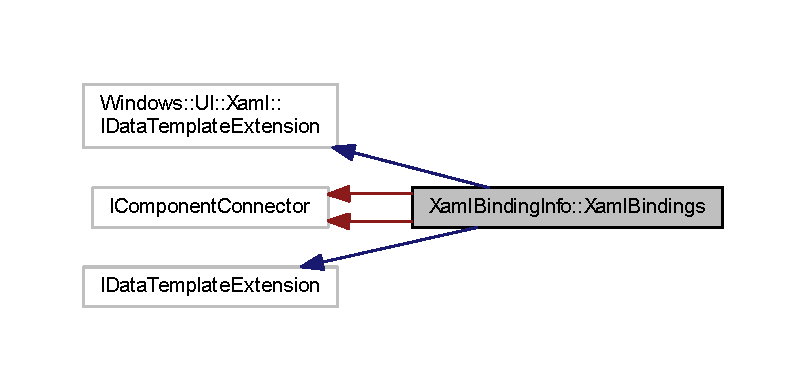
\includegraphics[width=350pt]{class_xaml_binding_info_1_1_xaml_bindings__inherit__graph}
\end{center}
\end{figure}


Collaboration diagram for Xaml\+Binding\+Info\+:\+:Xaml\+Bindings\+:\nopagebreak
\begin{figure}[H]
\begin{center}
\leavevmode
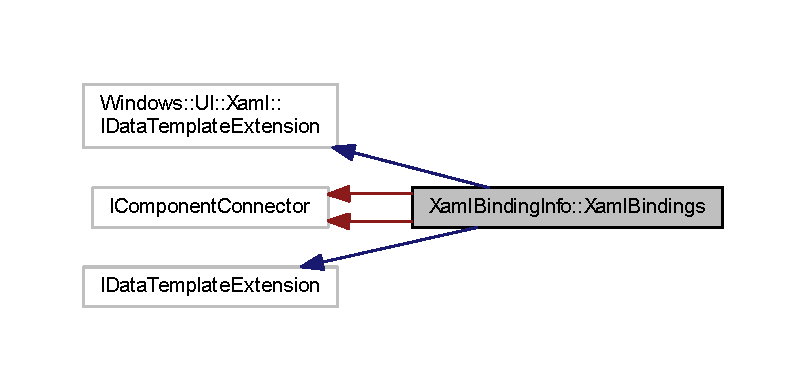
\includegraphics[width=350pt]{class_xaml_binding_info_1_1_xaml_bindings__coll__graph}
\end{center}
\end{figure}
\subsection*{Public Member Functions}
\begin{DoxyCompactItemize}
\item 
\mbox{\Hypertarget{class_xaml_binding_info_1_1_xaml_bindings_a949c24e21bb4968df1e313ab1a29ca0f}\label{class_xaml_binding_info_1_1_xaml_bindings_a949c24e21bb4968df1e313ab1a29ca0f}} 
virtual void {\bfseries Connect} (int connection\+Id, \+::Platform\+::\+Object$^\wedge$ target)
\item 
\mbox{\Hypertarget{class_xaml_binding_info_1_1_xaml_bindings_a596997845905d809ae11b635aef345e0}\label{class_xaml_binding_info_1_1_xaml_bindings_a596997845905d809ae11b635aef345e0}} 
virtual bool {\bfseries Process\+Binding} (unsigned int)
\item 
\mbox{\Hypertarget{class_xaml_binding_info_1_1_xaml_bindings_aa19559351b48ed6444cac4b04364cc4c}\label{class_xaml_binding_info_1_1_xaml_bindings_aa19559351b48ed6444cac4b04364cc4c}} 
virtual int {\bfseries Process\+Bindings} (\+::Windows\+::\+U\+I\+::\+Xaml\+::\+Controls\+::\+Container\+Content\+Changing\+Event\+Args$^\wedge$ args)
\item 
\mbox{\Hypertarget{class_xaml_binding_info_1_1_xaml_bindings_a35fa732801c8eb428cf9662ff8771d9f}\label{class_xaml_binding_info_1_1_xaml_bindings_a35fa732801c8eb428cf9662ff8771d9f}} 
virtual void {\bfseries Reset\+Template} ()
\item 
\mbox{\Hypertarget{class_xaml_binding_info_1_1_xaml_bindings_a949c24e21bb4968df1e313ab1a29ca0f}\label{class_xaml_binding_info_1_1_xaml_bindings_a949c24e21bb4968df1e313ab1a29ca0f}} 
virtual void {\bfseries Connect} (int connection\+Id, \+::Platform\+::\+Object$^\wedge$ target)
\item 
\mbox{\Hypertarget{class_xaml_binding_info_1_1_xaml_bindings_a596997845905d809ae11b635aef345e0}\label{class_xaml_binding_info_1_1_xaml_bindings_a596997845905d809ae11b635aef345e0}} 
virtual bool {\bfseries Process\+Binding} (unsigned int)
\item 
\mbox{\Hypertarget{class_xaml_binding_info_1_1_xaml_bindings_aa19559351b48ed6444cac4b04364cc4c}\label{class_xaml_binding_info_1_1_xaml_bindings_aa19559351b48ed6444cac4b04364cc4c}} 
virtual int {\bfseries Process\+Bindings} (\+::Windows\+::\+U\+I\+::\+Xaml\+::\+Controls\+::\+Container\+Content\+Changing\+Event\+Args$^\wedge$ args)
\item 
\mbox{\Hypertarget{class_xaml_binding_info_1_1_xaml_bindings_a35fa732801c8eb428cf9662ff8771d9f}\label{class_xaml_binding_info_1_1_xaml_bindings_a35fa732801c8eb428cf9662ff8771d9f}} 
virtual void {\bfseries Reset\+Template} ()
\end{DoxyCompactItemize}


\subsection{Detailed Description}


Definition at line 29 of file Xaml\+Binding\+Info.\+g.\+h.



The documentation for this class was generated from the following file\+:\begin{DoxyCompactItemize}
\item 
C\+:/\+Projects/\+Bergermeister\+Home/\+Console/\+Generated Files/Xaml\+Binding\+Info.\+g.\+h\end{DoxyCompactItemize}

\hypertarget{class_xaml_type_info_1_1_info_provider_1_1_xaml_member}{}\section{Xaml\+Type\+Info\+:\+:Info\+Provider\+:\+:Xaml\+Member Class Reference}
\label{class_xaml_type_info_1_1_info_provider_1_1_xaml_member}\index{Xaml\+Type\+Info\+::\+Info\+Provider\+::\+Xaml\+Member@{Xaml\+Type\+Info\+::\+Info\+Provider\+::\+Xaml\+Member}}


Inheritance diagram for Xaml\+Type\+Info\+:\+:Info\+Provider\+:\+:Xaml\+Member\+:\nopagebreak
\begin{figure}[H]
\begin{center}
\leavevmode
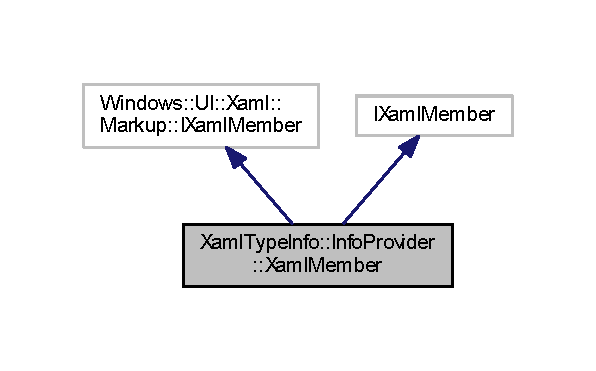
\includegraphics[width=286pt]{class_xaml_type_info_1_1_info_provider_1_1_xaml_member__inherit__graph}
\end{center}
\end{figure}


Collaboration diagram for Xaml\+Type\+Info\+:\+:Info\+Provider\+:\+:Xaml\+Member\+:\nopagebreak
\begin{figure}[H]
\begin{center}
\leavevmode
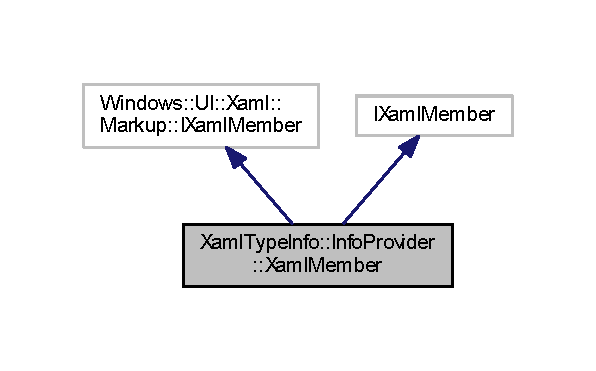
\includegraphics[width=286pt]{class_xaml_type_info_1_1_info_provider_1_1_xaml_member__coll__graph}
\end{center}
\end{figure}
\subsection*{Public Member Functions}
\begin{DoxyCompactItemize}
\item 
\mbox{\Hypertarget{class_xaml_type_info_1_1_info_provider_1_1_xaml_member_abd8aeffcd5cf9ab0de67f7cd21bb09e0}\label{class_xaml_type_info_1_1_info_provider_1_1_xaml_member_abd8aeffcd5cf9ab0de67f7cd21bb09e0}} 
virtual \+::Platform\+::\+Object $^\wedge$ {\bfseries Get\+Value} (\+::Platform\+::\+Object$^\wedge$ instance)
\item 
\mbox{\Hypertarget{class_xaml_type_info_1_1_info_provider_1_1_xaml_member_a091e60ae327bb36dece1558b14c889cc}\label{class_xaml_type_info_1_1_info_provider_1_1_xaml_member_a091e60ae327bb36dece1558b14c889cc}} 
virtual void {\bfseries Set\+Value} (\+::Platform\+::\+Object$^\wedge$ instance, \+::Platform\+::\+Object$^\wedge$ value)
\item 
\mbox{\Hypertarget{class_xaml_type_info_1_1_info_provider_1_1_xaml_member_a2c59558f3a5943b7c522686ef29afdce}\label{class_xaml_type_info_1_1_info_provider_1_1_xaml_member_a2c59558f3a5943b7c522686ef29afdce}} 
virtual \+::Platform\+::\+Object $^\wedge$ {\bfseries Get\+Value} (\+::Platform\+::\+Object$^\wedge$ instance)
\item 
\mbox{\Hypertarget{class_xaml_type_info_1_1_info_provider_1_1_xaml_member_a091e60ae327bb36dece1558b14c889cc}\label{class_xaml_type_info_1_1_info_provider_1_1_xaml_member_a091e60ae327bb36dece1558b14c889cc}} 
virtual void {\bfseries Set\+Value} (\+::Platform\+::\+Object$^\wedge$ instance, \+::Platform\+::\+Object$^\wedge$ value)
\end{DoxyCompactItemize}
\subsection*{Public Attributes}
\begin{DoxyCompactItemize}
\item 
virtual property \+::Platform\+::\+String $^\wedge$ {\bfseries Name}
\item 
virtual property \+::Windows\+::\+U\+I\+::\+Xaml\+::\+Markup\+::\+I\+Xaml\+Type $^\wedge$ {\bfseries Type}
\item 
virtual property \+::Windows\+::\+U\+I\+::\+Xaml\+::\+Markup\+::\+I\+Xaml\+Type $^\wedge$ {\bfseries Target\+Type}
\end{DoxyCompactItemize}
\subsection*{Properties}
\begin{DoxyCompactItemize}
\item 
\mbox{\Hypertarget{class_xaml_type_info_1_1_info_provider_1_1_xaml_member_acc8de4765b09acd4b6b8d2083adf501c}\label{class_xaml_type_info_1_1_info_provider_1_1_xaml_member_acc8de4765b09acd4b6b8d2083adf501c}} 
virtual bool {\bfseries Is\+Attachable}\hspace{0.3cm}{\ttfamily  \mbox{[}get, set\mbox{]}}
\item 
\mbox{\Hypertarget{class_xaml_type_info_1_1_info_provider_1_1_xaml_member_af1850c11a8e6df045cc88196df6d85e3}\label{class_xaml_type_info_1_1_info_provider_1_1_xaml_member_af1850c11a8e6df045cc88196df6d85e3}} 
virtual bool {\bfseries Is\+Dependency\+Property}\hspace{0.3cm}{\ttfamily  \mbox{[}get, set\mbox{]}}
\item 
\mbox{\Hypertarget{class_xaml_type_info_1_1_info_provider_1_1_xaml_member_a66b48fe9e8c22fe2e31b0dc3b102ef06}\label{class_xaml_type_info_1_1_info_provider_1_1_xaml_member_a66b48fe9e8c22fe2e31b0dc3b102ef06}} 
virtual bool {\bfseries Is\+Read\+Only}\hspace{0.3cm}{\ttfamily  \mbox{[}get, set\mbox{]}}
\end{DoxyCompactItemize}


\subsection{Detailed Description}


Definition at line 286 of file Xaml\+Type\+Info.\+g.\+h.



\subsection{Member Data Documentation}
\mbox{\Hypertarget{class_xaml_type_info_1_1_info_provider_1_1_xaml_member_a49ef07a113cfa90692716b5b110038f3}\label{class_xaml_type_info_1_1_info_provider_1_1_xaml_member_a49ef07a113cfa90692716b5b110038f3}} 
\index{Xaml\+Type\+Info\+::\+Info\+Provider\+::\+Xaml\+Member@{Xaml\+Type\+Info\+::\+Info\+Provider\+::\+Xaml\+Member}!Name@{Name}}
\index{Name@{Name}!Xaml\+Type\+Info\+::\+Info\+Provider\+::\+Xaml\+Member@{Xaml\+Type\+Info\+::\+Info\+Provider\+::\+Xaml\+Member}}
\subsubsection{\texorpdfstring{Name}{Name}}
{\footnotesize\ttfamily property\+::\+Platform\+::\+String Xaml\+Type\+Info\+::\+Info\+Provider\+::\+Xaml\+Member\+::\+Name}

{\bfseries Initial value\+:}
\begin{DoxyCode}
\{ 
                ::Platform::String^ \textcolor{keyword}{get}()
\end{DoxyCode}


Definition at line 317 of file Xaml\+Type\+Info.\+g.\+h.

\mbox{\Hypertarget{class_xaml_type_info_1_1_info_provider_1_1_xaml_member_aba768b49f071f01bf32e19d594b48026}\label{class_xaml_type_info_1_1_info_provider_1_1_xaml_member_aba768b49f071f01bf32e19d594b48026}} 
\index{Xaml\+Type\+Info\+::\+Info\+Provider\+::\+Xaml\+Member@{Xaml\+Type\+Info\+::\+Info\+Provider\+::\+Xaml\+Member}!Target\+Type@{Target\+Type}}
\index{Target\+Type@{Target\+Type}!Xaml\+Type\+Info\+::\+Info\+Provider\+::\+Xaml\+Member@{Xaml\+Type\+Info\+::\+Info\+Provider\+::\+Xaml\+Member}}
\subsubsection{\texorpdfstring{Target\+Type}{TargetType}}
{\footnotesize\ttfamily property\+::\+Windows\+::\+U\+I\+::\+Xaml\+::\+Markup\+::\+I\+Xaml\+Type Xaml\+Type\+Info\+::\+Info\+Provider\+::\+Xaml\+Member\+::\+Target\+Type}

{\bfseries Initial value\+:}
\begin{DoxyCode}
\{
                ::Windows::UI::Xaml::Markup::IXamlType^ \textcolor{keyword}{get}()
\end{DoxyCode}


Definition at line 327 of file Xaml\+Type\+Info.\+g.\+h.

\mbox{\Hypertarget{class_xaml_type_info_1_1_info_provider_1_1_xaml_member_a3562e6c2f5feb3c81fb14658fb250360}\label{class_xaml_type_info_1_1_info_provider_1_1_xaml_member_a3562e6c2f5feb3c81fb14658fb250360}} 
\index{Xaml\+Type\+Info\+::\+Info\+Provider\+::\+Xaml\+Member@{Xaml\+Type\+Info\+::\+Info\+Provider\+::\+Xaml\+Member}!Type@{Type}}
\index{Type@{Type}!Xaml\+Type\+Info\+::\+Info\+Provider\+::\+Xaml\+Member@{Xaml\+Type\+Info\+::\+Info\+Provider\+::\+Xaml\+Member}}
\subsubsection{\texorpdfstring{Type}{Type}}
{\footnotesize\ttfamily property\+::\+Windows\+::\+U\+I\+::\+Xaml\+::\+Markup\+::\+I\+Xaml\+Type Xaml\+Type\+Info\+::\+Info\+Provider\+::\+Xaml\+Member\+::\+Type}

{\bfseries Initial value\+:}
\begin{DoxyCode}
\{
                ::Windows::UI::Xaml::Markup::IXamlType^ \textcolor{keyword}{get}()
\end{DoxyCode}


Definition at line 322 of file Xaml\+Type\+Info.\+g.\+h.



The documentation for this class was generated from the following files\+:\begin{DoxyCompactItemize}
\item 
C\+:/\+Projects/\+Bergermeister\+Home/\+Console/\+Generated Files/Xaml\+Type\+Info.\+g.\+h\item 
C\+:/\+Projects/\+Bergermeister\+Home/\+Console/\+Generated Files/Xaml\+Type\+Info.\+Impl.\+g.\+cpp\end{DoxyCompactItemize}

\hypertarget{class_xaml_type_info_1_1_info_provider_1_1_xaml_system_base_type}{}\section{Xaml\+Type\+Info\+:\+:Info\+Provider\+:\+:Xaml\+System\+Base\+Type Class Reference}
\label{class_xaml_type_info_1_1_info_provider_1_1_xaml_system_base_type}\index{Xaml\+Type\+Info\+::\+Info\+Provider\+::\+Xaml\+System\+Base\+Type@{Xaml\+Type\+Info\+::\+Info\+Provider\+::\+Xaml\+System\+Base\+Type}}


Inheritance diagram for Xaml\+Type\+Info\+:\+:Info\+Provider\+:\+:Xaml\+System\+Base\+Type\+:\nopagebreak
\begin{figure}[H]
\begin{center}
\leavevmode
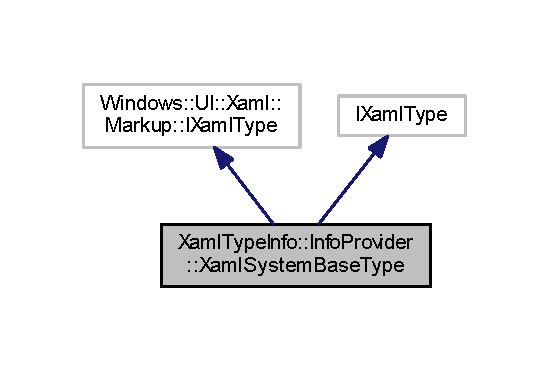
\includegraphics[width=264pt]{class_xaml_type_info_1_1_info_provider_1_1_xaml_system_base_type__inherit__graph}
\end{center}
\end{figure}


Collaboration diagram for Xaml\+Type\+Info\+:\+:Info\+Provider\+:\+:Xaml\+System\+Base\+Type\+:\nopagebreak
\begin{figure}[H]
\begin{center}
\leavevmode
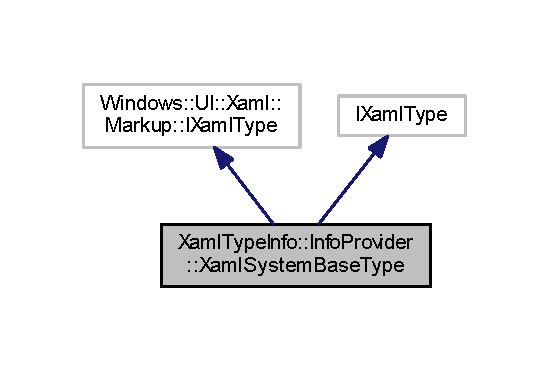
\includegraphics[width=264pt]{class_xaml_type_info_1_1_info_provider_1_1_xaml_system_base_type__coll__graph}
\end{center}
\end{figure}
\subsection*{Public Member Functions}
\begin{DoxyCompactItemize}
\item 
\mbox{\Hypertarget{class_xaml_type_info_1_1_info_provider_1_1_xaml_system_base_type_a7bc524ad414b526f74f4b1430950b43c}\label{class_xaml_type_info_1_1_info_provider_1_1_xaml_system_base_type_a7bc524ad414b526f74f4b1430950b43c}} 
virtual \+::Platform\+::\+Object $^\wedge$ {\bfseries Activate\+Instance} ()
\item 
\mbox{\Hypertarget{class_xaml_type_info_1_1_info_provider_1_1_xaml_system_base_type_a1897c34762f46b0b6ba1896dfe22b742}\label{class_xaml_type_info_1_1_info_provider_1_1_xaml_system_base_type_a1897c34762f46b0b6ba1896dfe22b742}} 
virtual \+::Windows\+::\+U\+I\+::\+Xaml\+::\+Markup\+::\+I\+Xaml\+Member $^\wedge$ {\bfseries Get\+Member} (\+::Platform\+::\+String$^\wedge$ name)
\item 
\mbox{\Hypertarget{class_xaml_type_info_1_1_info_provider_1_1_xaml_system_base_type_aaafca3b7939450d02d74df7fa930c623}\label{class_xaml_type_info_1_1_info_provider_1_1_xaml_system_base_type_aaafca3b7939450d02d74df7fa930c623}} 
virtual void {\bfseries Add\+To\+Vector} (\+::Platform\+::\+Object$^\wedge$ instance, \+::Platform\+::\+Object$^\wedge$ value)
\item 
\mbox{\Hypertarget{class_xaml_type_info_1_1_info_provider_1_1_xaml_system_base_type_a96244e1a7ed8813253abac0b606a68c6}\label{class_xaml_type_info_1_1_info_provider_1_1_xaml_system_base_type_a96244e1a7ed8813253abac0b606a68c6}} 
virtual void {\bfseries Add\+To\+Map} (\+::Platform\+::\+Object$^\wedge$ instance, \+::Platform\+::\+Object$^\wedge$ key, \+::Platform\+::\+Object$^\wedge$ value)
\item 
\mbox{\Hypertarget{class_xaml_type_info_1_1_info_provider_1_1_xaml_system_base_type_a622f1311cdaa7761b778a59e931c7420}\label{class_xaml_type_info_1_1_info_provider_1_1_xaml_system_base_type_a622f1311cdaa7761b778a59e931c7420}} 
virtual void {\bfseries Run\+Initializer} ()
\item 
\mbox{\Hypertarget{class_xaml_type_info_1_1_info_provider_1_1_xaml_system_base_type_a555d48692a6fd5e40fbe554c28b43dc2}\label{class_xaml_type_info_1_1_info_provider_1_1_xaml_system_base_type_a555d48692a6fd5e40fbe554c28b43dc2}} 
virtual \+::Platform\+::\+Object $^\wedge$ {\bfseries Create\+From\+String} (\+::Platform\+::\+String$^\wedge$ value)
\item 
\mbox{\Hypertarget{class_xaml_type_info_1_1_info_provider_1_1_xaml_system_base_type_aeefbd7181260daebb31bb4decbd88268}\label{class_xaml_type_info_1_1_info_provider_1_1_xaml_system_base_type_aeefbd7181260daebb31bb4decbd88268}} 
virtual \+::Platform\+::\+Object $^\wedge$ {\bfseries Activate\+Instance} ()
\item 
\mbox{\Hypertarget{class_xaml_type_info_1_1_info_provider_1_1_xaml_system_base_type_a694b9a55328fc1f366af9166e95423c0}\label{class_xaml_type_info_1_1_info_provider_1_1_xaml_system_base_type_a694b9a55328fc1f366af9166e95423c0}} 
virtual \+::Windows\+::\+U\+I\+::\+Xaml\+::\+Markup\+::\+I\+Xaml\+Member $^\wedge$ {\bfseries Get\+Member} (\+::Platform\+::\+String$^\wedge$ name)
\item 
\mbox{\Hypertarget{class_xaml_type_info_1_1_info_provider_1_1_xaml_system_base_type_aaafca3b7939450d02d74df7fa930c623}\label{class_xaml_type_info_1_1_info_provider_1_1_xaml_system_base_type_aaafca3b7939450d02d74df7fa930c623}} 
virtual void {\bfseries Add\+To\+Vector} (\+::Platform\+::\+Object$^\wedge$ instance, \+::Platform\+::\+Object$^\wedge$ value)
\item 
\mbox{\Hypertarget{class_xaml_type_info_1_1_info_provider_1_1_xaml_system_base_type_a96244e1a7ed8813253abac0b606a68c6}\label{class_xaml_type_info_1_1_info_provider_1_1_xaml_system_base_type_a96244e1a7ed8813253abac0b606a68c6}} 
virtual void {\bfseries Add\+To\+Map} (\+::Platform\+::\+Object$^\wedge$ instance, \+::Platform\+::\+Object$^\wedge$ key, \+::Platform\+::\+Object$^\wedge$ value)
\item 
\mbox{\Hypertarget{class_xaml_type_info_1_1_info_provider_1_1_xaml_system_base_type_a622f1311cdaa7761b778a59e931c7420}\label{class_xaml_type_info_1_1_info_provider_1_1_xaml_system_base_type_a622f1311cdaa7761b778a59e931c7420}} 
virtual void {\bfseries Run\+Initializer} ()
\item 
\mbox{\Hypertarget{class_xaml_type_info_1_1_info_provider_1_1_xaml_system_base_type_abb6dc9e86056b271c2b3ab9381b1fb84}\label{class_xaml_type_info_1_1_info_provider_1_1_xaml_system_base_type_abb6dc9e86056b271c2b3ab9381b1fb84}} 
virtual \+::Platform\+::\+Object $^\wedge$ {\bfseries Create\+From\+String} (\+::Platform\+::\+String$^\wedge$ value)
\end{DoxyCompactItemize}
\subsection*{Public Attributes}
\begin{DoxyCompactItemize}
\item 
virtual property \+::Windows\+::\+U\+I\+::\+Xaml\+::\+Markup\+::\+I\+Xaml\+Type $^\wedge$ {\bfseries Base\+Type}
\item 
virtual property \+::Windows\+::\+U\+I\+::\+Xaml\+::\+Markup\+::\+I\+Xaml\+Member $^\wedge$ {\bfseries Content\+Property}
\item 
virtual property \+::Platform\+::\+String $^\wedge$ {\bfseries Full\+Name}
\item 
virtual property \+::Platform\+::\+String $^\wedge$ {\bfseries Name}
\item 
virtual property \+::Windows\+::\+U\+I\+::\+Xaml\+::\+Markup\+::\+I\+Xaml\+Type $^\wedge$ {\bfseries Item\+Type}
\item 
virtual property \+::Windows\+::\+U\+I\+::\+Xaml\+::\+Markup\+::\+I\+Xaml\+Type $^\wedge$ {\bfseries Key\+Type}
\item 
virtual property \+::Windows\+::\+U\+I\+::\+Xaml\+::\+Interop\+::\+Type\+Name {\bfseries Underlying\+Type}
\end{DoxyCompactItemize}
\subsection*{Properties}
\begin{DoxyCompactItemize}
\item 
\mbox{\Hypertarget{class_xaml_type_info_1_1_info_provider_1_1_xaml_system_base_type_a6dd90c915857762f4913ff410c253d6d}\label{class_xaml_type_info_1_1_info_provider_1_1_xaml_system_base_type_a6dd90c915857762f4913ff410c253d6d}} 
virtual bool {\bfseries Is\+Array}\hspace{0.3cm}{\ttfamily  \mbox{[}get\mbox{]}}
\item 
\mbox{\Hypertarget{class_xaml_type_info_1_1_info_provider_1_1_xaml_system_base_type_a9720bcbb959020ea9be09a42e41ba50d}\label{class_xaml_type_info_1_1_info_provider_1_1_xaml_system_base_type_a9720bcbb959020ea9be09a42e41ba50d}} 
virtual bool {\bfseries Is\+Collection}\hspace{0.3cm}{\ttfamily  \mbox{[}get\mbox{]}}
\item 
\mbox{\Hypertarget{class_xaml_type_info_1_1_info_provider_1_1_xaml_system_base_type_a4395493313416b0c2bde8cba185cacff}\label{class_xaml_type_info_1_1_info_provider_1_1_xaml_system_base_type_a4395493313416b0c2bde8cba185cacff}} 
virtual bool {\bfseries Is\+Constructible}\hspace{0.3cm}{\ttfamily  \mbox{[}get\mbox{]}}
\item 
\mbox{\Hypertarget{class_xaml_type_info_1_1_info_provider_1_1_xaml_system_base_type_a69c21b2f22e743f2cfe16519184a2fec}\label{class_xaml_type_info_1_1_info_provider_1_1_xaml_system_base_type_a69c21b2f22e743f2cfe16519184a2fec}} 
virtual bool {\bfseries Is\+Dictionary}\hspace{0.3cm}{\ttfamily  \mbox{[}get\mbox{]}}
\item 
\mbox{\Hypertarget{class_xaml_type_info_1_1_info_provider_1_1_xaml_system_base_type_a88cf927b1d3f00208665fc36a239e4ee}\label{class_xaml_type_info_1_1_info_provider_1_1_xaml_system_base_type_a88cf927b1d3f00208665fc36a239e4ee}} 
virtual bool {\bfseries Is\+Markup\+Extension}\hspace{0.3cm}{\ttfamily  \mbox{[}get\mbox{]}}
\item 
\mbox{\Hypertarget{class_xaml_type_info_1_1_info_provider_1_1_xaml_system_base_type_a45cff85e6808c9e979a8e0e3486969c4}\label{class_xaml_type_info_1_1_info_provider_1_1_xaml_system_base_type_a45cff85e6808c9e979a8e0e3486969c4}} 
virtual bool {\bfseries Is\+Enum}\hspace{0.3cm}{\ttfamily  \mbox{[}get\mbox{]}}
\item 
\mbox{\Hypertarget{class_xaml_type_info_1_1_info_provider_1_1_xaml_system_base_type_a82a37d086e3f3d77ae6e7b0edc298993}\label{class_xaml_type_info_1_1_info_provider_1_1_xaml_system_base_type_a82a37d086e3f3d77ae6e7b0edc298993}} 
virtual bool {\bfseries Is\+System\+Type}\hspace{0.3cm}{\ttfamily  \mbox{[}get\mbox{]}}
\item 
\mbox{\Hypertarget{class_xaml_type_info_1_1_info_provider_1_1_xaml_system_base_type_ac4f01b414cc3ac7fba3dbab20a8989f6}\label{class_xaml_type_info_1_1_info_provider_1_1_xaml_system_base_type_ac4f01b414cc3ac7fba3dbab20a8989f6}} 
virtual bool {\bfseries Is\+Bindable}\hspace{0.3cm}{\ttfamily  \mbox{[}get\mbox{]}}
\end{DoxyCompactItemize}


\subsection{Detailed Description}


Definition at line 40 of file Xaml\+Type\+Info.\+g.\+h.



\subsection{Member Data Documentation}
\mbox{\Hypertarget{class_xaml_type_info_1_1_info_provider_1_1_xaml_system_base_type_aa97518aef4b7922035e75ee3ef34f425}\label{class_xaml_type_info_1_1_info_provider_1_1_xaml_system_base_type_aa97518aef4b7922035e75ee3ef34f425}} 
\index{Xaml\+Type\+Info\+::\+Info\+Provider\+::\+Xaml\+System\+Base\+Type@{Xaml\+Type\+Info\+::\+Info\+Provider\+::\+Xaml\+System\+Base\+Type}!Base\+Type@{Base\+Type}}
\index{Base\+Type@{Base\+Type}!Xaml\+Type\+Info\+::\+Info\+Provider\+::\+Xaml\+System\+Base\+Type@{Xaml\+Type\+Info\+::\+Info\+Provider\+::\+Xaml\+System\+Base\+Type}}
\subsubsection{\texorpdfstring{Base\+Type}{BaseType}}
{\footnotesize\ttfamily property\+::\+Windows\+::\+U\+I\+::\+Xaml\+::\+Markup\+::\+I\+Xaml\+Type Xaml\+Type\+Info\+::\+Info\+Provider\+::\+Xaml\+System\+Base\+Type\+::\+Base\+Type}

{\bfseries Initial value\+:}
\begin{DoxyCode}
\{
                ::Windows::UI::Xaml::Markup::IXamlType^ \textcolor{keyword}{get}()
\end{DoxyCode}


Definition at line 47 of file Xaml\+Type\+Info.\+g.\+h.

\mbox{\Hypertarget{class_xaml_type_info_1_1_info_provider_1_1_xaml_system_base_type_aa0afe4b2c59ae261902addaba1df5177}\label{class_xaml_type_info_1_1_info_provider_1_1_xaml_system_base_type_aa0afe4b2c59ae261902addaba1df5177}} 
\index{Xaml\+Type\+Info\+::\+Info\+Provider\+::\+Xaml\+System\+Base\+Type@{Xaml\+Type\+Info\+::\+Info\+Provider\+::\+Xaml\+System\+Base\+Type}!Content\+Property@{Content\+Property}}
\index{Content\+Property@{Content\+Property}!Xaml\+Type\+Info\+::\+Info\+Provider\+::\+Xaml\+System\+Base\+Type@{Xaml\+Type\+Info\+::\+Info\+Provider\+::\+Xaml\+System\+Base\+Type}}
\subsubsection{\texorpdfstring{Content\+Property}{ContentProperty}}
{\footnotesize\ttfamily property\+::\+Windows\+::\+U\+I\+::\+Xaml\+::\+Markup\+::\+I\+Xaml\+Member Xaml\+Type\+Info\+::\+Info\+Provider\+::\+Xaml\+System\+Base\+Type\+::\+Content\+Property}

{\bfseries Initial value\+:}
\begin{DoxyCode}
\{
                ::Windows::UI::Xaml::Markup::IXamlMember^ \textcolor{keyword}{get}()
\end{DoxyCode}


Definition at line 52 of file Xaml\+Type\+Info.\+g.\+h.

\mbox{\Hypertarget{class_xaml_type_info_1_1_info_provider_1_1_xaml_system_base_type_af4b9412b110614ec97de74d4c2884733}\label{class_xaml_type_info_1_1_info_provider_1_1_xaml_system_base_type_af4b9412b110614ec97de74d4c2884733}} 
\index{Xaml\+Type\+Info\+::\+Info\+Provider\+::\+Xaml\+System\+Base\+Type@{Xaml\+Type\+Info\+::\+Info\+Provider\+::\+Xaml\+System\+Base\+Type}!Full\+Name@{Full\+Name}}
\index{Full\+Name@{Full\+Name}!Xaml\+Type\+Info\+::\+Info\+Provider\+::\+Xaml\+System\+Base\+Type@{Xaml\+Type\+Info\+::\+Info\+Provider\+::\+Xaml\+System\+Base\+Type}}
\subsubsection{\texorpdfstring{Full\+Name}{FullName}}
{\footnotesize\ttfamily property\+::\+Platform\+::\+String Xaml\+Type\+Info\+::\+Info\+Provider\+::\+Xaml\+System\+Base\+Type\+::\+Full\+Name}

{\bfseries Initial value\+:}
\begin{DoxyCode}
\{
                ::Platform::String^ \textcolor{keyword}{get}()
\end{DoxyCode}


Definition at line 57 of file Xaml\+Type\+Info.\+g.\+h.

\mbox{\Hypertarget{class_xaml_type_info_1_1_info_provider_1_1_xaml_system_base_type_a5b0244721c000fdf757a66e690112822}\label{class_xaml_type_info_1_1_info_provider_1_1_xaml_system_base_type_a5b0244721c000fdf757a66e690112822}} 
\index{Xaml\+Type\+Info\+::\+Info\+Provider\+::\+Xaml\+System\+Base\+Type@{Xaml\+Type\+Info\+::\+Info\+Provider\+::\+Xaml\+System\+Base\+Type}!Item\+Type@{Item\+Type}}
\index{Item\+Type@{Item\+Type}!Xaml\+Type\+Info\+::\+Info\+Provider\+::\+Xaml\+System\+Base\+Type@{Xaml\+Type\+Info\+::\+Info\+Provider\+::\+Xaml\+System\+Base\+Type}}
\subsubsection{\texorpdfstring{Item\+Type}{ItemType}}
{\footnotesize\ttfamily property\+::\+Windows\+::\+U\+I\+::\+Xaml\+::\+Markup\+::\+I\+Xaml\+Type Xaml\+Type\+Info\+::\+Info\+Provider\+::\+Xaml\+System\+Base\+Type\+::\+Item\+Type}

{\bfseries Initial value\+:}
\begin{DoxyCode}
\{
                ::Windows::UI::Xaml::Markup::IXamlType^ \textcolor{keyword}{get}()
\end{DoxyCode}


Definition at line 107 of file Xaml\+Type\+Info.\+g.\+h.

\mbox{\Hypertarget{class_xaml_type_info_1_1_info_provider_1_1_xaml_system_base_type_a9012b6185609eb77880cb48416fd86dc}\label{class_xaml_type_info_1_1_info_provider_1_1_xaml_system_base_type_a9012b6185609eb77880cb48416fd86dc}} 
\index{Xaml\+Type\+Info\+::\+Info\+Provider\+::\+Xaml\+System\+Base\+Type@{Xaml\+Type\+Info\+::\+Info\+Provider\+::\+Xaml\+System\+Base\+Type}!Key\+Type@{Key\+Type}}
\index{Key\+Type@{Key\+Type}!Xaml\+Type\+Info\+::\+Info\+Provider\+::\+Xaml\+System\+Base\+Type@{Xaml\+Type\+Info\+::\+Info\+Provider\+::\+Xaml\+System\+Base\+Type}}
\subsubsection{\texorpdfstring{Key\+Type}{KeyType}}
{\footnotesize\ttfamily property\+::\+Windows\+::\+U\+I\+::\+Xaml\+::\+Markup\+::\+I\+Xaml\+Type Xaml\+Type\+Info\+::\+Info\+Provider\+::\+Xaml\+System\+Base\+Type\+::\+Key\+Type}

{\bfseries Initial value\+:}
\begin{DoxyCode}
\{
                ::Windows::UI::Xaml::Markup::IXamlType^ \textcolor{keyword}{get}()
\end{DoxyCode}


Definition at line 112 of file Xaml\+Type\+Info.\+g.\+h.

\mbox{\Hypertarget{class_xaml_type_info_1_1_info_provider_1_1_xaml_system_base_type_a44a6de0d0294e11103802d36c7a28d1f}\label{class_xaml_type_info_1_1_info_provider_1_1_xaml_system_base_type_a44a6de0d0294e11103802d36c7a28d1f}} 
\index{Xaml\+Type\+Info\+::\+Info\+Provider\+::\+Xaml\+System\+Base\+Type@{Xaml\+Type\+Info\+::\+Info\+Provider\+::\+Xaml\+System\+Base\+Type}!Name@{Name}}
\index{Name@{Name}!Xaml\+Type\+Info\+::\+Info\+Provider\+::\+Xaml\+System\+Base\+Type@{Xaml\+Type\+Info\+::\+Info\+Provider\+::\+Xaml\+System\+Base\+Type}}
\subsubsection{\texorpdfstring{Name}{Name}}
{\footnotesize\ttfamily property\+::\+Platform\+::\+String Xaml\+Type\+Info\+::\+Info\+Provider\+::\+Xaml\+System\+Base\+Type\+::\+Name}

{\bfseries Initial value\+:}
\begin{DoxyCode}
\{
                ::Platform::String^ \textcolor{keyword}{get}()
\end{DoxyCode}


Definition at line 62 of file Xaml\+Type\+Info.\+g.\+h.

\mbox{\Hypertarget{class_xaml_type_info_1_1_info_provider_1_1_xaml_system_base_type_abb659fe4aaa303e5309dd48ca3cfc45a}\label{class_xaml_type_info_1_1_info_provider_1_1_xaml_system_base_type_abb659fe4aaa303e5309dd48ca3cfc45a}} 
\index{Xaml\+Type\+Info\+::\+Info\+Provider\+::\+Xaml\+System\+Base\+Type@{Xaml\+Type\+Info\+::\+Info\+Provider\+::\+Xaml\+System\+Base\+Type}!Underlying\+Type@{Underlying\+Type}}
\index{Underlying\+Type@{Underlying\+Type}!Xaml\+Type\+Info\+::\+Info\+Provider\+::\+Xaml\+System\+Base\+Type@{Xaml\+Type\+Info\+::\+Info\+Provider\+::\+Xaml\+System\+Base\+Type}}
\subsubsection{\texorpdfstring{Underlying\+Type}{UnderlyingType}}
{\footnotesize\ttfamily property\+::\+Windows\+::\+U\+I\+::\+Xaml\+::\+Interop\+::\+Type\+Name Xaml\+Type\+Info\+::\+Info\+Provider\+::\+Xaml\+System\+Base\+Type\+::\+Underlying\+Type}

{\bfseries Initial value\+:}
\begin{DoxyCode}
\{
                ::Windows::UI::Xaml::Interop::TypeName \textcolor{keyword}{get}()
\end{DoxyCode}


Definition at line 117 of file Xaml\+Type\+Info.\+g.\+h.



The documentation for this class was generated from the following files\+:\begin{DoxyCompactItemize}
\item 
C\+:/\+Projects/\+Bergermeister\+Home/\+Console/\+Generated Files/Xaml\+Type\+Info.\+g.\+h\item 
C\+:/\+Projects/\+Bergermeister\+Home/\+Console/\+Generated Files/Xaml\+Type\+Info.\+Impl.\+g.\+cpp\end{DoxyCompactItemize}

\hypertarget{class_xaml_type_info_1_1_info_provider_1_1_xaml_type_info_provider}{}\section{Xaml\+Type\+Info\+:\+:Info\+Provider\+:\+:Xaml\+Type\+Info\+Provider Class Reference}
\label{class_xaml_type_info_1_1_info_provider_1_1_xaml_type_info_provider}\index{Xaml\+Type\+Info\+::\+Info\+Provider\+::\+Xaml\+Type\+Info\+Provider@{Xaml\+Type\+Info\+::\+Info\+Provider\+::\+Xaml\+Type\+Info\+Provider}}
\subsection*{Public Member Functions}
\begin{DoxyCompactItemize}
\item 
\mbox{\Hypertarget{class_xaml_type_info_1_1_info_provider_1_1_xaml_type_info_provider_a884b800e91fa2666bc4154420eefccf2}\label{class_xaml_type_info_1_1_info_provider_1_1_xaml_type_info_provider_a884b800e91fa2666bc4154420eefccf2}} 
\+::Windows\+::\+U\+I\+::\+Xaml\+::\+Markup\+::\+I\+Xaml\+Type $^\wedge$ {\bfseries Get\+Xaml\+Type\+By\+Name} (\+::Platform\+::\+String$^\wedge$ type\+Name)
\item 
\mbox{\Hypertarget{class_xaml_type_info_1_1_info_provider_1_1_xaml_type_info_provider_a61a7092d4197201ffb0904659c1ea89a}\label{class_xaml_type_info_1_1_info_provider_1_1_xaml_type_info_provider_a61a7092d4197201ffb0904659c1ea89a}} 
\+::Windows\+::\+U\+I\+::\+Xaml\+::\+Markup\+::\+I\+Xaml\+Type $^\wedge$ {\bfseries Get\+Xaml\+Type\+By\+Type} (\+::Windows\+::\+U\+I\+::\+Xaml\+::\+Interop\+::\+Type\+Name t)
\item 
\mbox{\Hypertarget{class_xaml_type_info_1_1_info_provider_1_1_xaml_type_info_provider_af84a49d4e30e1ed575cc8b2ac9c47e54}\label{class_xaml_type_info_1_1_info_provider_1_1_xaml_type_info_provider_af84a49d4e30e1ed575cc8b2ac9c47e54}} 
\+::Windows\+::\+U\+I\+::\+Xaml\+::\+Markup\+::\+I\+Xaml\+Member $^\wedge$ {\bfseries Get\+Member\+By\+Long\+Name} (\+::Platform\+::\+String$^\wedge$ long\+Member\+Name)
\item 
\mbox{\Hypertarget{class_xaml_type_info_1_1_info_provider_1_1_xaml_type_info_provider_a9b6eea2111a9c404fc281b94389c5b87}\label{class_xaml_type_info_1_1_info_provider_1_1_xaml_type_info_provider_a9b6eea2111a9c404fc281b94389c5b87}} 
void {\bfseries Add\+Other\+Provider} (\+::Windows\+::\+U\+I\+::\+Xaml\+::\+Markup\+::\+I\+Xaml\+Metadata\+Provider$^\wedge$ other\+Provider)
\item 
\mbox{\Hypertarget{class_xaml_type_info_1_1_info_provider_1_1_xaml_type_info_provider_a37556c5ef8fae3ce58b97c95b06c0ea9}\label{class_xaml_type_info_1_1_info_provider_1_1_xaml_type_info_provider_a37556c5ef8fae3ce58b97c95b06c0ea9}} 
\+::Windows\+::\+U\+I\+::\+Xaml\+::\+Markup\+::\+I\+Xaml\+Type $^\wedge$ {\bfseries Get\+Xaml\+Type\+By\+Name} (\+::Platform\+::\+String$^\wedge$ type\+Name)
\item 
\mbox{\Hypertarget{class_xaml_type_info_1_1_info_provider_1_1_xaml_type_info_provider_abd06d7d1579ab8549518aecfdaee2993}\label{class_xaml_type_info_1_1_info_provider_1_1_xaml_type_info_provider_abd06d7d1579ab8549518aecfdaee2993}} 
\+::Windows\+::\+U\+I\+::\+Xaml\+::\+Markup\+::\+I\+Xaml\+Type $^\wedge$ {\bfseries Get\+Xaml\+Type\+By\+Type} (\+::Windows\+::\+U\+I\+::\+Xaml\+::\+Interop\+::\+Type\+Name t)
\item 
\mbox{\Hypertarget{class_xaml_type_info_1_1_info_provider_1_1_xaml_type_info_provider_a340eaef5dc634cc6ea25f4b40c723c3a}\label{class_xaml_type_info_1_1_info_provider_1_1_xaml_type_info_provider_a340eaef5dc634cc6ea25f4b40c723c3a}} 
\+::Windows\+::\+U\+I\+::\+Xaml\+::\+Markup\+::\+I\+Xaml\+Member $^\wedge$ {\bfseries Get\+Member\+By\+Long\+Name} (\+::Platform\+::\+String$^\wedge$ long\+Member\+Name)
\item 
\mbox{\Hypertarget{class_xaml_type_info_1_1_info_provider_1_1_xaml_type_info_provider_a9b6eea2111a9c404fc281b94389c5b87}\label{class_xaml_type_info_1_1_info_provider_1_1_xaml_type_info_provider_a9b6eea2111a9c404fc281b94389c5b87}} 
void {\bfseries Add\+Other\+Provider} (\+::Windows\+::\+U\+I\+::\+Xaml\+::\+Markup\+::\+I\+Xaml\+Metadata\+Provider$^\wedge$ other\+Provider)
\end{DoxyCompactItemize}


\subsection{Detailed Description}


Definition at line 16 of file Xaml\+Type\+Info.\+g.\+h.



The documentation for this class was generated from the following files\+:\begin{DoxyCompactItemize}
\item 
C\+:/\+Projects/\+Bergermeister\+Home/\+Console/\+Generated Files/Xaml\+Type\+Info.\+g.\+h\item 
C\+:/\+Projects/\+Bergermeister\+Home/\+Console/\+Generated Files/Xaml\+Type\+Info.\+Impl.\+g.\+cpp\item 
C\+:/\+Projects/\+Bergermeister\+Home/\+Thermostat/\+Generated Files/Xaml\+Type\+Info.\+g.\+cpp\end{DoxyCompactItemize}

\hypertarget{class_xaml_type_info_1_1_info_provider_1_1_xaml_user_type}{}\section{Xaml\+Type\+Info\+:\+:Info\+Provider\+:\+:Xaml\+User\+Type Class Reference}
\label{class_xaml_type_info_1_1_info_provider_1_1_xaml_user_type}\index{Xaml\+Type\+Info\+::\+Info\+Provider\+::\+Xaml\+User\+Type@{Xaml\+Type\+Info\+::\+Info\+Provider\+::\+Xaml\+User\+Type}}


Inheritance diagram for Xaml\+Type\+Info\+:\+:Info\+Provider\+:\+:Xaml\+User\+Type\+:\nopagebreak
\begin{figure}[H]
\begin{center}
\leavevmode
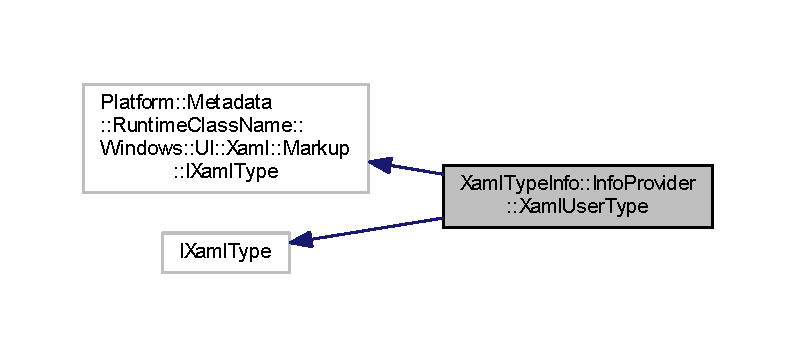
\includegraphics[width=350pt]{class_xaml_type_info_1_1_info_provider_1_1_xaml_user_type__inherit__graph}
\end{center}
\end{figure}


Collaboration diagram for Xaml\+Type\+Info\+:\+:Info\+Provider\+:\+:Xaml\+User\+Type\+:\nopagebreak
\begin{figure}[H]
\begin{center}
\leavevmode
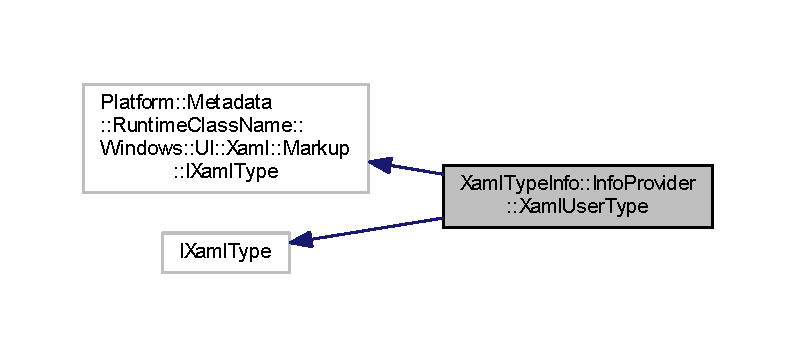
\includegraphics[width=350pt]{class_xaml_type_info_1_1_info_provider_1_1_xaml_user_type__coll__graph}
\end{center}
\end{figure}
\subsection*{Public Member Functions}
\begin{DoxyCompactItemize}
\item 
\mbox{\Hypertarget{class_xaml_type_info_1_1_info_provider_1_1_xaml_user_type_a4c1839fa1be2287b32c86ab5d45b2af3}\label{class_xaml_type_info_1_1_info_provider_1_1_xaml_user_type_a4c1839fa1be2287b32c86ab5d45b2af3}} 
virtual \+::Windows\+::\+U\+I\+::\+Xaml\+::\+Markup\+::\+I\+Xaml\+Member $^\wedge$ {\bfseries Get\+Member} (\+::Platform\+::\+String$^\wedge$ name)
\item 
\mbox{\Hypertarget{class_xaml_type_info_1_1_info_provider_1_1_xaml_user_type_ab23d0c633fe997f65be39c9486152408}\label{class_xaml_type_info_1_1_info_provider_1_1_xaml_user_type_ab23d0c633fe997f65be39c9486152408}} 
virtual \+::Platform\+::\+Object $^\wedge$ {\bfseries Activate\+Instance} ()
\item 
\mbox{\Hypertarget{class_xaml_type_info_1_1_info_provider_1_1_xaml_user_type_aa2d1cf0cc528940509545ebdeb61926c}\label{class_xaml_type_info_1_1_info_provider_1_1_xaml_user_type_aa2d1cf0cc528940509545ebdeb61926c}} 
virtual void {\bfseries Add\+To\+Map} (\+::Platform\+::\+Object$^\wedge$ instance, \+::Platform\+::\+Object$^\wedge$ key, \+::Platform\+::\+Object$^\wedge$ value)
\item 
\mbox{\Hypertarget{class_xaml_type_info_1_1_info_provider_1_1_xaml_user_type_a93b639b8ab3dd00a61776a99a0da3f54}\label{class_xaml_type_info_1_1_info_provider_1_1_xaml_user_type_a93b639b8ab3dd00a61776a99a0da3f54}} 
virtual void {\bfseries Add\+To\+Vector} (\+::Platform\+::\+Object$^\wedge$ instance, \+::Platform\+::\+Object$^\wedge$ value)
\item 
\mbox{\Hypertarget{class_xaml_type_info_1_1_info_provider_1_1_xaml_user_type_a27ab5687ea814468d9382aa7e6502465}\label{class_xaml_type_info_1_1_info_provider_1_1_xaml_user_type_a27ab5687ea814468d9382aa7e6502465}} 
virtual void {\bfseries Run\+Initializer} ()
\item 
\mbox{\Hypertarget{class_xaml_type_info_1_1_info_provider_1_1_xaml_user_type_a7657d00c04fc9d34365f79d064227ba1}\label{class_xaml_type_info_1_1_info_provider_1_1_xaml_user_type_a7657d00c04fc9d34365f79d064227ba1}} 
virtual \+::Platform\+::\+Object $^\wedge$ {\bfseries Create\+From\+String} (\+::Platform\+::\+String$^\wedge$ value)
\item 
\mbox{\Hypertarget{class_xaml_type_info_1_1_info_provider_1_1_xaml_user_type_ac876d5510485e0fd2e91b1a866c1d54d}\label{class_xaml_type_info_1_1_info_provider_1_1_xaml_user_type_ac876d5510485e0fd2e91b1a866c1d54d}} 
virtual \+::Windows\+::\+U\+I\+::\+Xaml\+::\+Markup\+::\+I\+Xaml\+Member $^\wedge$ {\bfseries Get\+Member} (\+::Platform\+::\+String$^\wedge$ name)
\item 
\mbox{\Hypertarget{class_xaml_type_info_1_1_info_provider_1_1_xaml_user_type_a6d0a15b5a83f03b7a37ebc450662a205}\label{class_xaml_type_info_1_1_info_provider_1_1_xaml_user_type_a6d0a15b5a83f03b7a37ebc450662a205}} 
virtual \+::Platform\+::\+Object $^\wedge$ {\bfseries Activate\+Instance} ()
\item 
\mbox{\Hypertarget{class_xaml_type_info_1_1_info_provider_1_1_xaml_user_type_aa2d1cf0cc528940509545ebdeb61926c}\label{class_xaml_type_info_1_1_info_provider_1_1_xaml_user_type_aa2d1cf0cc528940509545ebdeb61926c}} 
virtual void {\bfseries Add\+To\+Map} (\+::Platform\+::\+Object$^\wedge$ instance, \+::Platform\+::\+Object$^\wedge$ key, \+::Platform\+::\+Object$^\wedge$ value)
\item 
\mbox{\Hypertarget{class_xaml_type_info_1_1_info_provider_1_1_xaml_user_type_a93b639b8ab3dd00a61776a99a0da3f54}\label{class_xaml_type_info_1_1_info_provider_1_1_xaml_user_type_a93b639b8ab3dd00a61776a99a0da3f54}} 
virtual void {\bfseries Add\+To\+Vector} (\+::Platform\+::\+Object$^\wedge$ instance, \+::Platform\+::\+Object$^\wedge$ value)
\item 
\mbox{\Hypertarget{class_xaml_type_info_1_1_info_provider_1_1_xaml_user_type_a27ab5687ea814468d9382aa7e6502465}\label{class_xaml_type_info_1_1_info_provider_1_1_xaml_user_type_a27ab5687ea814468d9382aa7e6502465}} 
virtual void {\bfseries Run\+Initializer} ()
\item 
\mbox{\Hypertarget{class_xaml_type_info_1_1_info_provider_1_1_xaml_user_type_a889a00c934bfc7d5366f218dd3f50e48}\label{class_xaml_type_info_1_1_info_provider_1_1_xaml_user_type_a889a00c934bfc7d5366f218dd3f50e48}} 
virtual \+::Platform\+::\+Object $^\wedge$ {\bfseries Create\+From\+String} (\+::Platform\+::\+String$^\wedge$ value)
\end{DoxyCompactItemize}
\subsection*{Public Attributes}
\begin{DoxyCompactItemize}
\item 
virtual property \+::Platform\+::\+String $^\wedge$ {\bfseries Full\+Name}
\item 
virtual property \+::Platform\+::\+String $^\wedge$ {\bfseries Name}
\item 
virtual property \+::Windows\+::\+U\+I\+::\+Xaml\+::\+Interop\+::\+Type\+Name {\bfseries Underlying\+Type}
\item 
virtual property \+::Windows\+::\+U\+I\+::\+Xaml\+::\+Markup\+::\+I\+Xaml\+Type $^\wedge$ {\bfseries Base\+Type}
\item 
virtual property \+::Windows\+::\+U\+I\+::\+Xaml\+::\+Markup\+::\+I\+Xaml\+Member $^\wedge$ {\bfseries Content\+Property}
\item 
virtual property \+::Windows\+::\+U\+I\+::\+Xaml\+::\+Markup\+::\+I\+Xaml\+Type $^\wedge$ {\bfseries Item\+Type}
\item 
virtual property \+::Windows\+::\+U\+I\+::\+Xaml\+::\+Markup\+::\+I\+Xaml\+Type $^\wedge$ {\bfseries Key\+Type}
\end{DoxyCompactItemize}
\subsection*{Properties}
\begin{DoxyCompactItemize}
\item 
\mbox{\Hypertarget{class_xaml_type_info_1_1_info_provider_1_1_xaml_user_type_ad334f792ef4910ed2d36c6b65dda2e4b}\label{class_xaml_type_info_1_1_info_provider_1_1_xaml_user_type_ad334f792ef4910ed2d36c6b65dda2e4b}} 
virtual bool {\bfseries Is\+System\+Type}\hspace{0.3cm}{\ttfamily  \mbox{[}get\mbox{]}}
\item 
\mbox{\Hypertarget{class_xaml_type_info_1_1_info_provider_1_1_xaml_user_type_ae50864bc731a88748e2900be23bea67e}\label{class_xaml_type_info_1_1_info_provider_1_1_xaml_user_type_ae50864bc731a88748e2900be23bea67e}} 
virtual bool {\bfseries Is\+Array}\hspace{0.3cm}{\ttfamily  \mbox{[}get, set\mbox{]}}
\item 
\mbox{\Hypertarget{class_xaml_type_info_1_1_info_provider_1_1_xaml_user_type_afe23cd8567621d0f1b73d820ba16661b}\label{class_xaml_type_info_1_1_info_provider_1_1_xaml_user_type_afe23cd8567621d0f1b73d820ba16661b}} 
virtual bool {\bfseries Is\+Collection}\hspace{0.3cm}{\ttfamily  \mbox{[}get\mbox{]}}
\item 
\mbox{\Hypertarget{class_xaml_type_info_1_1_info_provider_1_1_xaml_user_type_ab4c1b7a5c932b0d200740406f70d1844}\label{class_xaml_type_info_1_1_info_provider_1_1_xaml_user_type_ab4c1b7a5c932b0d200740406f70d1844}} 
virtual bool {\bfseries Is\+Constructible}\hspace{0.3cm}{\ttfamily  \mbox{[}get\mbox{]}}
\item 
\mbox{\Hypertarget{class_xaml_type_info_1_1_info_provider_1_1_xaml_user_type_a611953c59013e34b80a13293ff63d59c}\label{class_xaml_type_info_1_1_info_provider_1_1_xaml_user_type_a611953c59013e34b80a13293ff63d59c}} 
virtual bool {\bfseries Is\+Dictionary}\hspace{0.3cm}{\ttfamily  \mbox{[}get\mbox{]}}
\item 
\mbox{\Hypertarget{class_xaml_type_info_1_1_info_provider_1_1_xaml_user_type_a6b4cce8b831bf6b0e1d29da25e7763f2}\label{class_xaml_type_info_1_1_info_provider_1_1_xaml_user_type_a6b4cce8b831bf6b0e1d29da25e7763f2}} 
virtual bool {\bfseries Is\+Markup\+Extension}\hspace{0.3cm}{\ttfamily  \mbox{[}get, set\mbox{]}}
\item 
\mbox{\Hypertarget{class_xaml_type_info_1_1_info_provider_1_1_xaml_user_type_aa12ec3e05d9426ca25a5e6f185965133}\label{class_xaml_type_info_1_1_info_provider_1_1_xaml_user_type_aa12ec3e05d9426ca25a5e6f185965133}} 
virtual bool {\bfseries Is\+Enum}\hspace{0.3cm}{\ttfamily  \mbox{[}get, set\mbox{]}}
\item 
\mbox{\Hypertarget{class_xaml_type_info_1_1_info_provider_1_1_xaml_user_type_ac9c45117680e53e00098ee9490c09b93}\label{class_xaml_type_info_1_1_info_provider_1_1_xaml_user_type_ac9c45117680e53e00098ee9490c09b93}} 
virtual bool {\bfseries Is\+Bindable}\hspace{0.3cm}{\ttfamily  \mbox{[}get, set\mbox{]}}
\item 
\mbox{\Hypertarget{class_xaml_type_info_1_1_info_provider_1_1_xaml_user_type_affd75cdc104291f57d99ba498c60a247}\label{class_xaml_type_info_1_1_info_provider_1_1_xaml_user_type_affd75cdc104291f57d99ba498c60a247}} 
bool {\bfseries Is\+Return\+Type\+Stub}\hspace{0.3cm}{\ttfamily  \mbox{[}get, set\mbox{]}}
\item 
\mbox{\Hypertarget{class_xaml_type_info_1_1_info_provider_1_1_xaml_user_type_a7bd48d31945050a6efccdea405693865}\label{class_xaml_type_info_1_1_info_provider_1_1_xaml_user_type_a7bd48d31945050a6efccdea405693865}} 
bool {\bfseries Is\+Local\+Type}\hspace{0.3cm}{\ttfamily  \mbox{[}get, set\mbox{]}}
\end{DoxyCompactItemize}


\subsection{Detailed Description}


Definition at line 132 of file Xaml\+Type\+Info.\+g.\+h.



\subsection{Member Data Documentation}
\mbox{\Hypertarget{class_xaml_type_info_1_1_info_provider_1_1_xaml_user_type_a8f8a691f4ca24641dd43829ecddc1e6b}\label{class_xaml_type_info_1_1_info_provider_1_1_xaml_user_type_a8f8a691f4ca24641dd43829ecddc1e6b}} 
\index{Xaml\+Type\+Info\+::\+Info\+Provider\+::\+Xaml\+User\+Type@{Xaml\+Type\+Info\+::\+Info\+Provider\+::\+Xaml\+User\+Type}!Base\+Type@{Base\+Type}}
\index{Base\+Type@{Base\+Type}!Xaml\+Type\+Info\+::\+Info\+Provider\+::\+Xaml\+User\+Type@{Xaml\+Type\+Info\+::\+Info\+Provider\+::\+Xaml\+User\+Type}}
\subsubsection{\texorpdfstring{Base\+Type}{BaseType}}
{\footnotesize\ttfamily property\+::\+Windows\+::\+U\+I\+::\+Xaml\+::\+Markup\+::\+I\+Xaml\+Type Xaml\+Type\+Info\+::\+Info\+Provider\+::\+Xaml\+User\+Type\+::\+Base\+Type}

{\bfseries Initial value\+:}
\begin{DoxyCode}
\{ 
                ::Windows::UI::Xaml::Markup::IXamlType^ \textcolor{keyword}{get}()
\end{DoxyCode}


Definition at line 160 of file Xaml\+Type\+Info.\+g.\+h.

\mbox{\Hypertarget{class_xaml_type_info_1_1_info_provider_1_1_xaml_user_type_ade211767c5690abfb557f603c02e7528}\label{class_xaml_type_info_1_1_info_provider_1_1_xaml_user_type_ade211767c5690abfb557f603c02e7528}} 
\index{Xaml\+Type\+Info\+::\+Info\+Provider\+::\+Xaml\+User\+Type@{Xaml\+Type\+Info\+::\+Info\+Provider\+::\+Xaml\+User\+Type}!Content\+Property@{Content\+Property}}
\index{Content\+Property@{Content\+Property}!Xaml\+Type\+Info\+::\+Info\+Provider\+::\+Xaml\+User\+Type@{Xaml\+Type\+Info\+::\+Info\+Provider\+::\+Xaml\+User\+Type}}
\subsubsection{\texorpdfstring{Content\+Property}{ContentProperty}}
{\footnotesize\ttfamily property\+::\+Windows\+::\+U\+I\+::\+Xaml\+::\+Markup\+::\+I\+Xaml\+Member Xaml\+Type\+Info\+::\+Info\+Provider\+::\+Xaml\+User\+Type\+::\+Content\+Property}

{\bfseries Initial value\+:}
\begin{DoxyCode}
\{ 
                ::Windows::UI::Xaml::Markup::IXamlMember^ \textcolor{keyword}{get}()
\end{DoxyCode}


Definition at line 204 of file Xaml\+Type\+Info.\+g.\+h.

\mbox{\Hypertarget{class_xaml_type_info_1_1_info_provider_1_1_xaml_user_type_a2980a74482f9f20d62e24a091b72d096}\label{class_xaml_type_info_1_1_info_provider_1_1_xaml_user_type_a2980a74482f9f20d62e24a091b72d096}} 
\index{Xaml\+Type\+Info\+::\+Info\+Provider\+::\+Xaml\+User\+Type@{Xaml\+Type\+Info\+::\+Info\+Provider\+::\+Xaml\+User\+Type}!Full\+Name@{Full\+Name}}
\index{Full\+Name@{Full\+Name}!Xaml\+Type\+Info\+::\+Info\+Provider\+::\+Xaml\+User\+Type@{Xaml\+Type\+Info\+::\+Info\+Provider\+::\+Xaml\+User\+Type}}
\subsubsection{\texorpdfstring{Full\+Name}{FullName}}
{\footnotesize\ttfamily property\+::\+Platform\+::\+String Xaml\+Type\+Info\+::\+Info\+Provider\+::\+Xaml\+User\+Type\+::\+Full\+Name}

{\bfseries Initial value\+:}
\begin{DoxyCode}
\{
                ::Platform::String^ \textcolor{keyword}{get}()
\end{DoxyCode}


Definition at line 140 of file Xaml\+Type\+Info.\+g.\+h.

\mbox{\Hypertarget{class_xaml_type_info_1_1_info_provider_1_1_xaml_user_type_a59724917c3bbf71f7c641d4b9d4b7cb6}\label{class_xaml_type_info_1_1_info_provider_1_1_xaml_user_type_a59724917c3bbf71f7c641d4b9d4b7cb6}} 
\index{Xaml\+Type\+Info\+::\+Info\+Provider\+::\+Xaml\+User\+Type@{Xaml\+Type\+Info\+::\+Info\+Provider\+::\+Xaml\+User\+Type}!Item\+Type@{Item\+Type}}
\index{Item\+Type@{Item\+Type}!Xaml\+Type\+Info\+::\+Info\+Provider\+::\+Xaml\+User\+Type@{Xaml\+Type\+Info\+::\+Info\+Provider\+::\+Xaml\+User\+Type}}
\subsubsection{\texorpdfstring{Item\+Type}{ItemType}}
{\footnotesize\ttfamily property\+::\+Windows\+::\+U\+I\+::\+Xaml\+::\+Markup\+::\+I\+Xaml\+Type Xaml\+Type\+Info\+::\+Info\+Provider\+::\+Xaml\+User\+Type\+::\+Item\+Type}

{\bfseries Initial value\+:}
\begin{DoxyCode}
\{ 
                ::Windows::UI::Xaml::Markup::IXamlType^ \textcolor{keyword}{get}()
\end{DoxyCode}


Definition at line 209 of file Xaml\+Type\+Info.\+g.\+h.

\mbox{\Hypertarget{class_xaml_type_info_1_1_info_provider_1_1_xaml_user_type_a2afcdd6aa7f0f45728c5d4ef0e0d25f5}\label{class_xaml_type_info_1_1_info_provider_1_1_xaml_user_type_a2afcdd6aa7f0f45728c5d4ef0e0d25f5}} 
\index{Xaml\+Type\+Info\+::\+Info\+Provider\+::\+Xaml\+User\+Type@{Xaml\+Type\+Info\+::\+Info\+Provider\+::\+Xaml\+User\+Type}!Key\+Type@{Key\+Type}}
\index{Key\+Type@{Key\+Type}!Xaml\+Type\+Info\+::\+Info\+Provider\+::\+Xaml\+User\+Type@{Xaml\+Type\+Info\+::\+Info\+Provider\+::\+Xaml\+User\+Type}}
\subsubsection{\texorpdfstring{Key\+Type}{KeyType}}
{\footnotesize\ttfamily property\+::\+Windows\+::\+U\+I\+::\+Xaml\+::\+Markup\+::\+I\+Xaml\+Type Xaml\+Type\+Info\+::\+Info\+Provider\+::\+Xaml\+User\+Type\+::\+Key\+Type}

{\bfseries Initial value\+:}
\begin{DoxyCode}
\{ 
                ::Windows::UI::Xaml::Markup::IXamlType^ \textcolor{keyword}{get}()
\end{DoxyCode}


Definition at line 214 of file Xaml\+Type\+Info.\+g.\+h.

\mbox{\Hypertarget{class_xaml_type_info_1_1_info_provider_1_1_xaml_user_type_ae4f73351219be7832cb30b118ed7f257}\label{class_xaml_type_info_1_1_info_provider_1_1_xaml_user_type_ae4f73351219be7832cb30b118ed7f257}} 
\index{Xaml\+Type\+Info\+::\+Info\+Provider\+::\+Xaml\+User\+Type@{Xaml\+Type\+Info\+::\+Info\+Provider\+::\+Xaml\+User\+Type}!Name@{Name}}
\index{Name@{Name}!Xaml\+Type\+Info\+::\+Info\+Provider\+::\+Xaml\+User\+Type@{Xaml\+Type\+Info\+::\+Info\+Provider\+::\+Xaml\+User\+Type}}
\subsubsection{\texorpdfstring{Name}{Name}}
{\footnotesize\ttfamily property\+::\+Platform\+::\+String Xaml\+Type\+Info\+::\+Info\+Provider\+::\+Xaml\+User\+Type\+::\+Name}

{\bfseries Initial value\+:}
\begin{DoxyCode}
\{
                ::Platform::String^ \textcolor{keyword}{get}()
\end{DoxyCode}


Definition at line 145 of file Xaml\+Type\+Info.\+g.\+h.

\mbox{\Hypertarget{class_xaml_type_info_1_1_info_provider_1_1_xaml_user_type_aa5bdf0da240db6feabb8ae26953c57cd}\label{class_xaml_type_info_1_1_info_provider_1_1_xaml_user_type_aa5bdf0da240db6feabb8ae26953c57cd}} 
\index{Xaml\+Type\+Info\+::\+Info\+Provider\+::\+Xaml\+User\+Type@{Xaml\+Type\+Info\+::\+Info\+Provider\+::\+Xaml\+User\+Type}!Underlying\+Type@{Underlying\+Type}}
\index{Underlying\+Type@{Underlying\+Type}!Xaml\+Type\+Info\+::\+Info\+Provider\+::\+Xaml\+User\+Type@{Xaml\+Type\+Info\+::\+Info\+Provider\+::\+Xaml\+User\+Type}}
\subsubsection{\texorpdfstring{Underlying\+Type}{UnderlyingType}}
{\footnotesize\ttfamily property\+::\+Windows\+::\+U\+I\+::\+Xaml\+::\+Interop\+::\+Type\+Name Xaml\+Type\+Info\+::\+Info\+Provider\+::\+Xaml\+User\+Type\+::\+Underlying\+Type}

{\bfseries Initial value\+:}
\begin{DoxyCode}
\{
                ::Windows::UI::Xaml::Interop::TypeName \textcolor{keyword}{get}()
\end{DoxyCode}


Definition at line 150 of file Xaml\+Type\+Info.\+g.\+h.



The documentation for this class was generated from the following files\+:\begin{DoxyCompactItemize}
\item 
C\+:/\+Projects/\+Bergermeister\+Home/\+Console/\+Generated Files/Xaml\+Type\+Info.\+g.\+h\item 
C\+:/\+Projects/\+Bergermeister\+Home/\+Console/\+Generated Files/Xaml\+Type\+Info.\+Impl.\+g.\+cpp\end{DoxyCompactItemize}

\chapter{File Documentation}
\hypertarget{_alert_8h}{}\section{C\+:/\+Users/edwar/\+Projects/\+Bergermeister\+Home/\+Software/\+Common/inc/\+Notification/\+Alert.h File Reference}
\label{_alert_8h}\index{C\+:/\+Users/edwar/\+Projects/\+Bergermeister\+Home/\+Software/\+Common/inc/\+Notification/\+Alert.\+h@{C\+:/\+Users/edwar/\+Projects/\+Bergermeister\+Home/\+Software/\+Common/inc/\+Notification/\+Alert.\+h}}


Package interface for the Alert Class.  


{\ttfamily \#include $<$Types.\+h$>$}\newline
{\ttfamily \#include $<$Component\textbackslash{}\+Model.\+h$>$}\newline
{\ttfamily \#include $<$Notification\textbackslash{}\+Component\+Id.\+h$>$}\newline
{\ttfamily \#include $<$Notification\textbackslash{}\+Identifier.\+h$>$}\newline
{\ttfamily \#include $<$Notification\textbackslash{}\+Status.\+h$>$}\newline
Include dependency graph for Alert.\+h\+:
\nopagebreak
\begin{figure}[H]
\begin{center}
\leavevmode
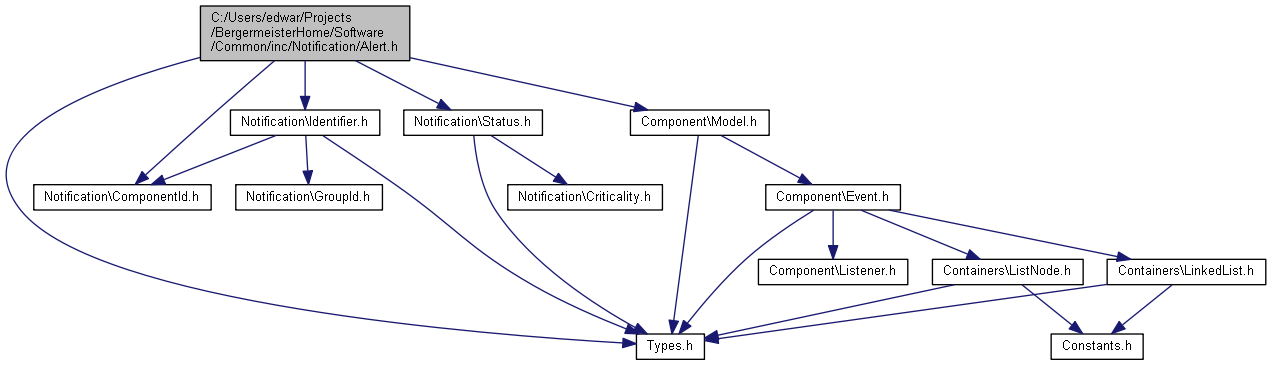
\includegraphics[width=350pt]{_alert_8h__incl}
\end{center}
\end{figure}
This graph shows which files directly or indirectly include this file\+:
\nopagebreak
\begin{figure}[H]
\begin{center}
\leavevmode
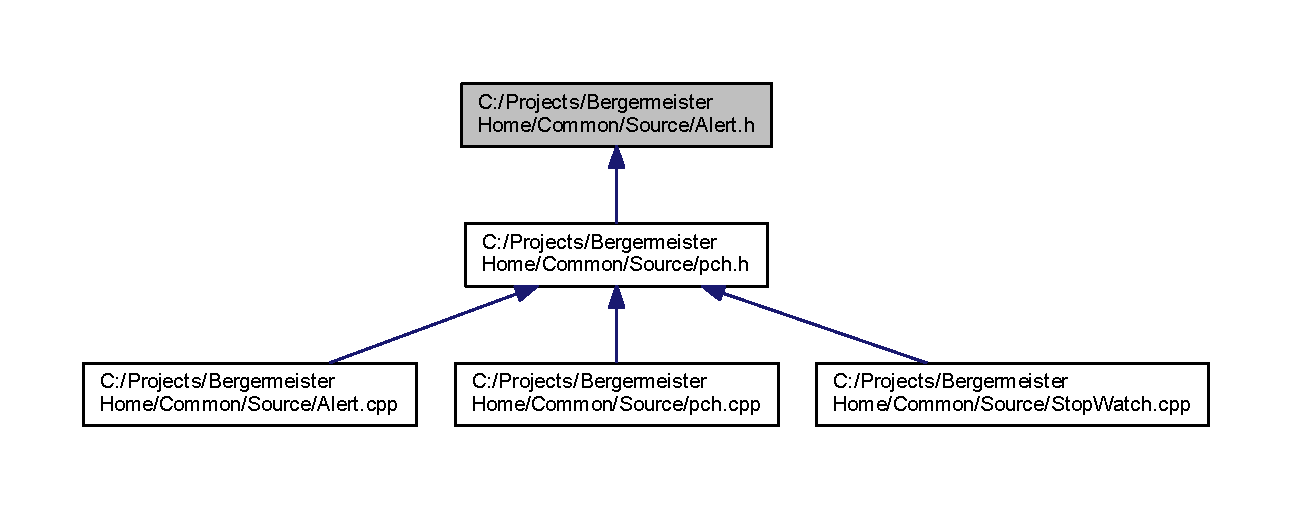
\includegraphics[width=248pt]{_alert_8h__dep__incl}
\end{center}
\end{figure}
\subsection*{Classes}
\begin{DoxyCompactItemize}
\item 
class \mbox{\hyperlink{class_g_n_common_1_1_n_notification_1_1_tc_alert}{G\+N\+Common\+::\+N\+Notification\+::\+Tc\+Alert}}
\end{DoxyCompactItemize}
\subsection*{Namespaces}
\begin{DoxyCompactItemize}
\item 
 \mbox{\hyperlink{namespace_g_n_common}{G\+N\+Common}}
\begin{DoxyCompactList}\small\item\em Namespace containing Common components and infrastrucutre. \end{DoxyCompactList}\item 
 \mbox{\hyperlink{namespace_g_n_common_1_1_n_notification}{G\+N\+Common\+::\+N\+Notification}}
\begin{DoxyCompactList}\small\item\em Namespace containing system Alerts. \end{DoxyCompactList}\end{DoxyCompactItemize}


\subsection{Detailed Description}
Package interface for the Alert Class. 



Definition in file \mbox{\hyperlink{_alert_8h_source}{Alert.\+h}}.


\hypertarget{_types_8h}{}\section{C\+:/\+Users/edwar/\+Projects/\+Bergermeister\+Home/\+Software/\+Common/inc/\+Types.h File Reference}
\label{_types_8h}\index{C\+:/\+Users/edwar/\+Projects/\+Bergermeister\+Home/\+Software/\+Common/inc/\+Types.\+h@{C\+:/\+Users/edwar/\+Projects/\+Bergermeister\+Home/\+Software/\+Common/inc/\+Types.\+h}}


Commnon Framework namespace, type definitions, and coding style guide Defines the common namespace (\mbox{\hyperlink{namespace_g_n_common}{G\+N\+Common}}), common primitive types, and provides the style guide to be used.  


This graph shows which files directly or indirectly include this file\+:
\nopagebreak
\begin{figure}[H]
\begin{center}
\leavevmode
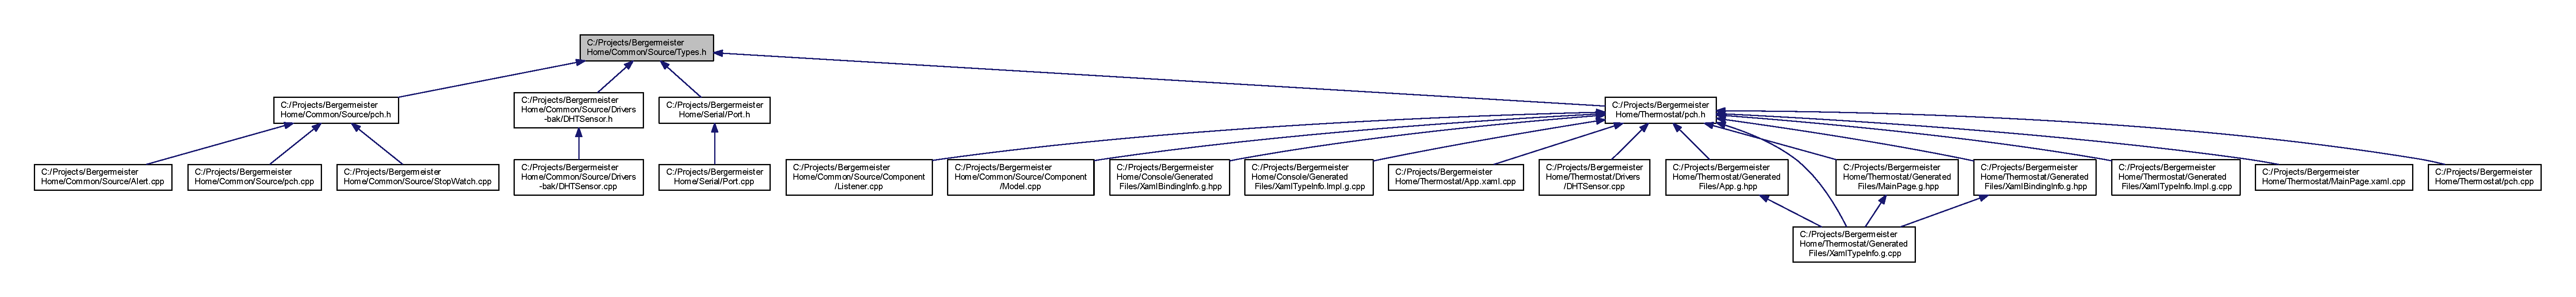
\includegraphics[width=350pt]{_types_8h__dep__incl}
\end{center}
\end{figure}
\subsection*{Namespaces}
\begin{DoxyCompactItemize}
\item 
 \mbox{\hyperlink{namespace_g_n_common}{G\+N\+Common}}
\begin{DoxyCompactList}\small\item\em Namespace containing Common components and infrastrucutre. \end{DoxyCompactList}\end{DoxyCompactItemize}
\subsection*{Typedefs}
\begin{DoxyCompactItemize}
\item 
typedef bool \mbox{\hyperlink{namespace_g_n_common_a8115dc7ed53b6e5b52e6bfde1632ea74}{G\+N\+Common\+::\+Tb8}}
\item 
typedef char \mbox{\hyperlink{namespace_g_n_common_a2d8d4c56e54519697c6ee80cc1ceda76}{G\+N\+Common\+::\+Tc8}}
\item 
typedef signed char \mbox{\hyperlink{namespace_g_n_common_a9bac2aa36db6d72a3e59b1869adf3668}{G\+N\+Common\+::\+Ti8}}
\item 
typedef unsigned char \mbox{\hyperlink{namespace_g_n_common_a7939e251ddbf5d3a31832dcfdc8bde39}{G\+N\+Common\+::\+Tu8}}
\item 
typedef signed short \mbox{\hyperlink{namespace_g_n_common_ab9a9a6aa84751cec965d8b6676318a65}{G\+N\+Common\+::\+Ti16}}
\item 
typedef unsigned short \mbox{\hyperlink{namespace_g_n_common_a7f651a58155939d1e0e2bf2164fbfdbf}{G\+N\+Common\+::\+Tu16}}
\item 
typedef signed long \mbox{\hyperlink{namespace_g_n_common_ad1f094ce51908947ac3d31355b560d55}{G\+N\+Common\+::\+Ti32}}
\item 
typedef unsigned long \mbox{\hyperlink{namespace_g_n_common_a941b527ef318f318aed7903dc832b7e4}{G\+N\+Common\+::\+Tu32}}
\item 
typedef signed long long \mbox{\hyperlink{namespace_g_n_common_ad0a34f67eefe81cfbd0e515bba246d9d}{G\+N\+Common\+::\+Ti64}}
\item 
typedef unsigned long long \mbox{\hyperlink{namespace_g_n_common_a9404ee6090c788ae70aebd1436ceb97d}{G\+N\+Common\+::\+Tu64}}
\item 
typedef float \mbox{\hyperlink{namespace_g_n_common_ae4ffdde6236eb7578669b280a5d1634d}{G\+N\+Common\+::\+Tf32}}
\item 
typedef double \mbox{\hyperlink{namespace_g_n_common_a73af96f1663fd8fc5741bcbc5b1427e4}{G\+N\+Common\+::\+Tf64}}
\end{DoxyCompactItemize}


\subsection{Detailed Description}
Commnon Framework namespace, type definitions, and coding style guide Defines the common namespace (\mbox{\hyperlink{namespace_g_n_common}{G\+N\+Common}}), common primitive types, and provides the style guide to be used. 

\begin{DoxyVerb}* Style Guide
*
*  (S)cope:                                
*                | Priv  |  Pub  | Global |
*                |-------|-------|--------|
* Class Variable |   v   |   V   |  ----  |
* Stack Variable |   k   |  ---  |  ----  | 
*       Argument |   a   |  ---  |  ----  |
*        Typedef |   t   |   T   |   GT   |
*   Constant ROM |   x   |   X   |   GX   |
*         Method |   m   |   M   |   GM   |
*                                          
*  (T)ype:                                 
*           | Prefix |                     
*           |--------|                     
*      Tb8 |    b   |                     
*      Tc8 |    c   |                     
*      Ti8 |    c   |                     
*      Tu8 |   uc   |                     
*     Ti16 |    s   |                     
*     Tu16 |   us   |                     
*     Ti32 |    i   |                     
*     Tu32 |   ui   |                     
*     Ti64 |    l   |                     
*     Tu64 |   ul   |                     
*     Tf32 |    f   |                     
*     Tf64 |    d   |                     
*                                          
*  (O)perator:                             
*               | Prefix |                 
*               |--------|                 
*     pointer   |    p   |                 
*     reference |    r   |                 
*                                          
*  Naming Convention:                      
*     STOCamelCaseName                     
*     GMFunctionGlobal
* \end{DoxyVerb}
 

Definition in file \mbox{\hyperlink{_types_8h_source}{Types.\+h}}.


%--- End generated contents ---

% Index
\backmatter
\newpage
\phantomsection
\clearemptydoublepage
\addcontentsline{toc}{chapter}{Index}
\printindex

\end{document}
